\chapter{Search for higgsino pair production}
\label{chap:ewk_prod}

This chapter presents a search for higgsino pair production, with decay to Higgs or $Z$ boson, 
focusing on the final states with four bottom quarks and \met. 
Two complementary searches target this signal model: the ``high-mass'' search,
which is the focus of this chapter, is optimized for 
cases with higgsinos heavy enough to produce sizable \met, while the ``low-mass'' search 
targets lower higgsino masses.
Section \ref{sec:ewk:sig} describes the signal models used to optimize and interpret the analysis. 
Section \ref{sec:ewk:sigbkg} discusses the strategy for the reconstruction of the candidate Higgs bosons in the event, 
and the variables that allow us to separate signal and background events. 
The definition of the analysis regions are presented in Sections \ref{sec:ewk:SR} and 
\ref{sec:ewk:CRVR}, 
while Section \ref{sec:ewk:bkgcomp} discusses the background composition. 
Section \ref{sec:ewk:dataMC} shows the comparison between data and simulation in a kinematic regime close to that of the analysis regions. 
Section \ref{sec:ewk:syst} discusses the systematic uncertainties that are included in the analysis, and Section \ref{sec:ewk:results} 
presents the results. 
The interpretation of the results in terms of model-independent and model-dependent limits is presented in Section \ref{sec:ewk:interp}. 
The low-mass search is briefly described in Section \ref{sec:ewk:LM}, and Section \ref{sec:ewk:HMLM}  
presents the combined results of the two searches. 


\section{Signal Model}
\label{sec:ewk:sig}

This analysis studies the simplified model shown in Figure \ref{fig:feyn}, targeting primarily the decays via Higgs boson.
These are models of \gls{ggm} \cite{Meade:2008wd,Cheung:2007es,Dine:1981gu,AlvarezGaume:1981wy,Nappi:1982hm} 
(already discussed in Section \ref{sec:susybreaking})
or \gls{gmsb} \cite{Dimopoulos:1996vz,Matchev:1999ft} where 
the lightest neutralino is the \gls{nlsp}, and decays promptly to the gravitino ($\gravino$), which is the \gls{lsp}, and 
a \gls{sm} boson. 

\begin{figure}[htbp]
	\centering
	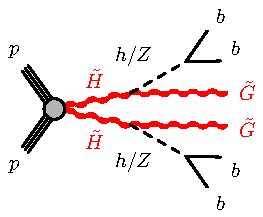
\includegraphics[width=0.35\textwidth]{figures/ewk_prod/varie/N1N1-hhGG-bbbb_Z}
	\caption{Diagram for the simplified model considered in the analysis. The primary interpretation of the analysis is the decay via Higgs bosons, but decays via varied branching ratios to $Z$ bosons are also studied. The production of the \hino\ occurs
via mass-degenerate pairs of charginos or neutralinos, which decay to the \ninoone\ and immeasurably low momentum particles.} 
	\label{fig:feyn}
\end{figure}

As discussed in Section \ref{sec:theo:mssm} \gls{susy} predicts five Higgs bosons. 
Their superpartners (higgsinos) mix with the superpartners of the electroweak gauge bosons to form charginos and neutralinos.

In models where the the lightest neutralinos and charginos are dominated by the higgsino component, the four lightest charginos 
and neutralinos are nearly degenerate \cite{Papucci:2011wy,Barbieri:2009ev,Han:2014kaa} and ordered as: $m_{\tilde\chi^0_1}~<~m_{\tilde\chi^\pm_1}~<~m_{\tilde\chi^0_2}$.
These models are particularly interesting because they arise in the limit where $|\mu| < |M_1|, |M_2$|, which is the same limit 
that minimizes the fine tuning problem in the Higgs sector of the \gls{mssm}.

In the case of a higgsino-like neutralino, the direct production of a \ninoone\ninoone\ pair is suppressed, and the production cross-section is dominated by 
\ninoone\ninotwo, \ninoone\chinoonepm, \ninotwo\chinoonepm, and \chinoonep\chinoonem production.
The \ninotwo and \chinoonepm then decay to the \ninoone and soft particles that can not be detected (originating from the 
decay of off-shell $W$ and $Z$ bosons), therefore all of these production processes give practically the same final state as 
\ninoone\ninoone\  pair production. 

Since in this chapter we consider only the case where the lightest neutralino is dominated by the higgsino component,
we will use interchangeably the notation \ninoone or \hino to indicate it.  
We consider only the case where the lifetime of the \hino is very short and it decays promptly to a Higgs boson or a Z boson and the \gravino;
this is the case when the mass of the mediators of \gls{susy} breaking is relatively small (smaller than $\approx 10^7$ GeV), 
while for higher mediator masses the \gls{nlsp} acquires a finite lifetime, and can decay in the detector or pass
 through the full detector without decaying. 

The analysis described in this thesis targets events where the \gravino is produced with enough transverse momentum to lead to 
sizable \met. This is the case when the higgsinos have intermediate or high mass.
This search is not sensitive to events where the higgsino mass is close to the mass of the Higgs boson, and therefore 
the signal events have very little \met and do not satisfy the \met trigger requirement.
These events are the focus of a dedicated analysis whose results are here briefly discussed in Section \ref{sec:ewk:LM}.


\subsection{Signal cross-section}

The signal cross-section is computed for the pure higgsino case, at \gls{nlo} plus \gls{nll} precision, assuming that
\ninoone, \ninotwo and \chinoonepm are degenarate and that all the other \gls{susy} particles decouple \cite{Fuks:2012qx,Fuks:2013vua}.
The nominal cross-section and its uncertainty are taken from an envelope of two cross-section predictions using different \gls{pdf} sets, 
and it is 3830 $\pm$ 160 fb at $\mhino = 150$ GeV, while it decreases to 1.8 $\pm$ 0.2 fb at $\mhino = 900$ GeV. 

\subsection{Higgsino decay modes}

This search is optimized to target cases where both \hino decay promptly to a Higgs boson and a gravitino with 100\% \gls{br}.
This is not the case in realistic models, where the decays of a short-lived higgsino in \gls{ggm} scenarios  
can be to a photon, a $Z$ boson or a Higgs boson with 
\gls{br} that depends on the choice of the parameters.
As discussed in Ref. \cite{Meade:2009qv}, the partial width of the three decays of the \ninoone is:

\begin{eqnarray}
\label{eqn:brfhi}
\Gamma(\tilde\chi_1^0\to \tilde G+\gamma)&=& {1\over2}(s_\beta+\eta c_\beta)^2\left({c_Ws_W(M_1-M_2)m_Z\over M_1 M_2}\right)^2 {\cal A} \;,
\nonumber\\
 \Gamma(\tilde\chi_1^0\to \tilde G+Z)&=&{1\over4}(s_\beta+\eta c_\beta)^2\left(1 - \frac{m_Z^2}{m^2_{\tilde{\chi}^0_1}}\right)^4 {\cal A} \;,\\
  \Gamma(\tilde\chi_1^0\to \tilde G+h)&=&{1\over4}(s_\beta-\eta c_\beta)^2\left(1 - \frac{m_h^2}{m^2_{\tilde{\chi}^0_1}}\right)^4 {\cal A} \;. \nonumber
\end{eqnarray}

\noindent In Equation \ref{eqn:brfhi}, ${\cal A}$ is a parameter related to the higgsino lifetime:
\begin{equation}
\label{eqn:decaylength}
{\cal A} = \frac{m^5_{\tilde{\chi}^0_1}}{16\pi F_0^2} \approx \left(\frac{m_{\tilde{\chi}^0_1}}{100~{\rm GeV}}\right)^5 \left(\frac{100~\rm{TeV}}{\sqrt{F_0}}\right)^4 \frac{1}{0.1~{\rm mm}} \;,
\end{equation}

\noindent $s_\beta$ and $c_\beta$ are the sine and cosine of the angle whose tangent is 
the ratio of the up-type to down-type Higgs \glspl{vev}, 
$\eta$ represents the relative sign of the coefficients 
of the two \glspl{vev} in the linear combination that constitutes \ninoone,
$M_1$ and $M_2$ are the bino and wino mass parameters respectively, and 
$F_0$ is the \gls{vev} of the \gls{susy}-breaking $F$-term, the fundamental scale of \gls{susy} breaking.
The three \glspl{br} for different choices of the parameters are shown in Figure \ref{fig:higgsinoBR}.

\begin{figure}[h]
	\centering
	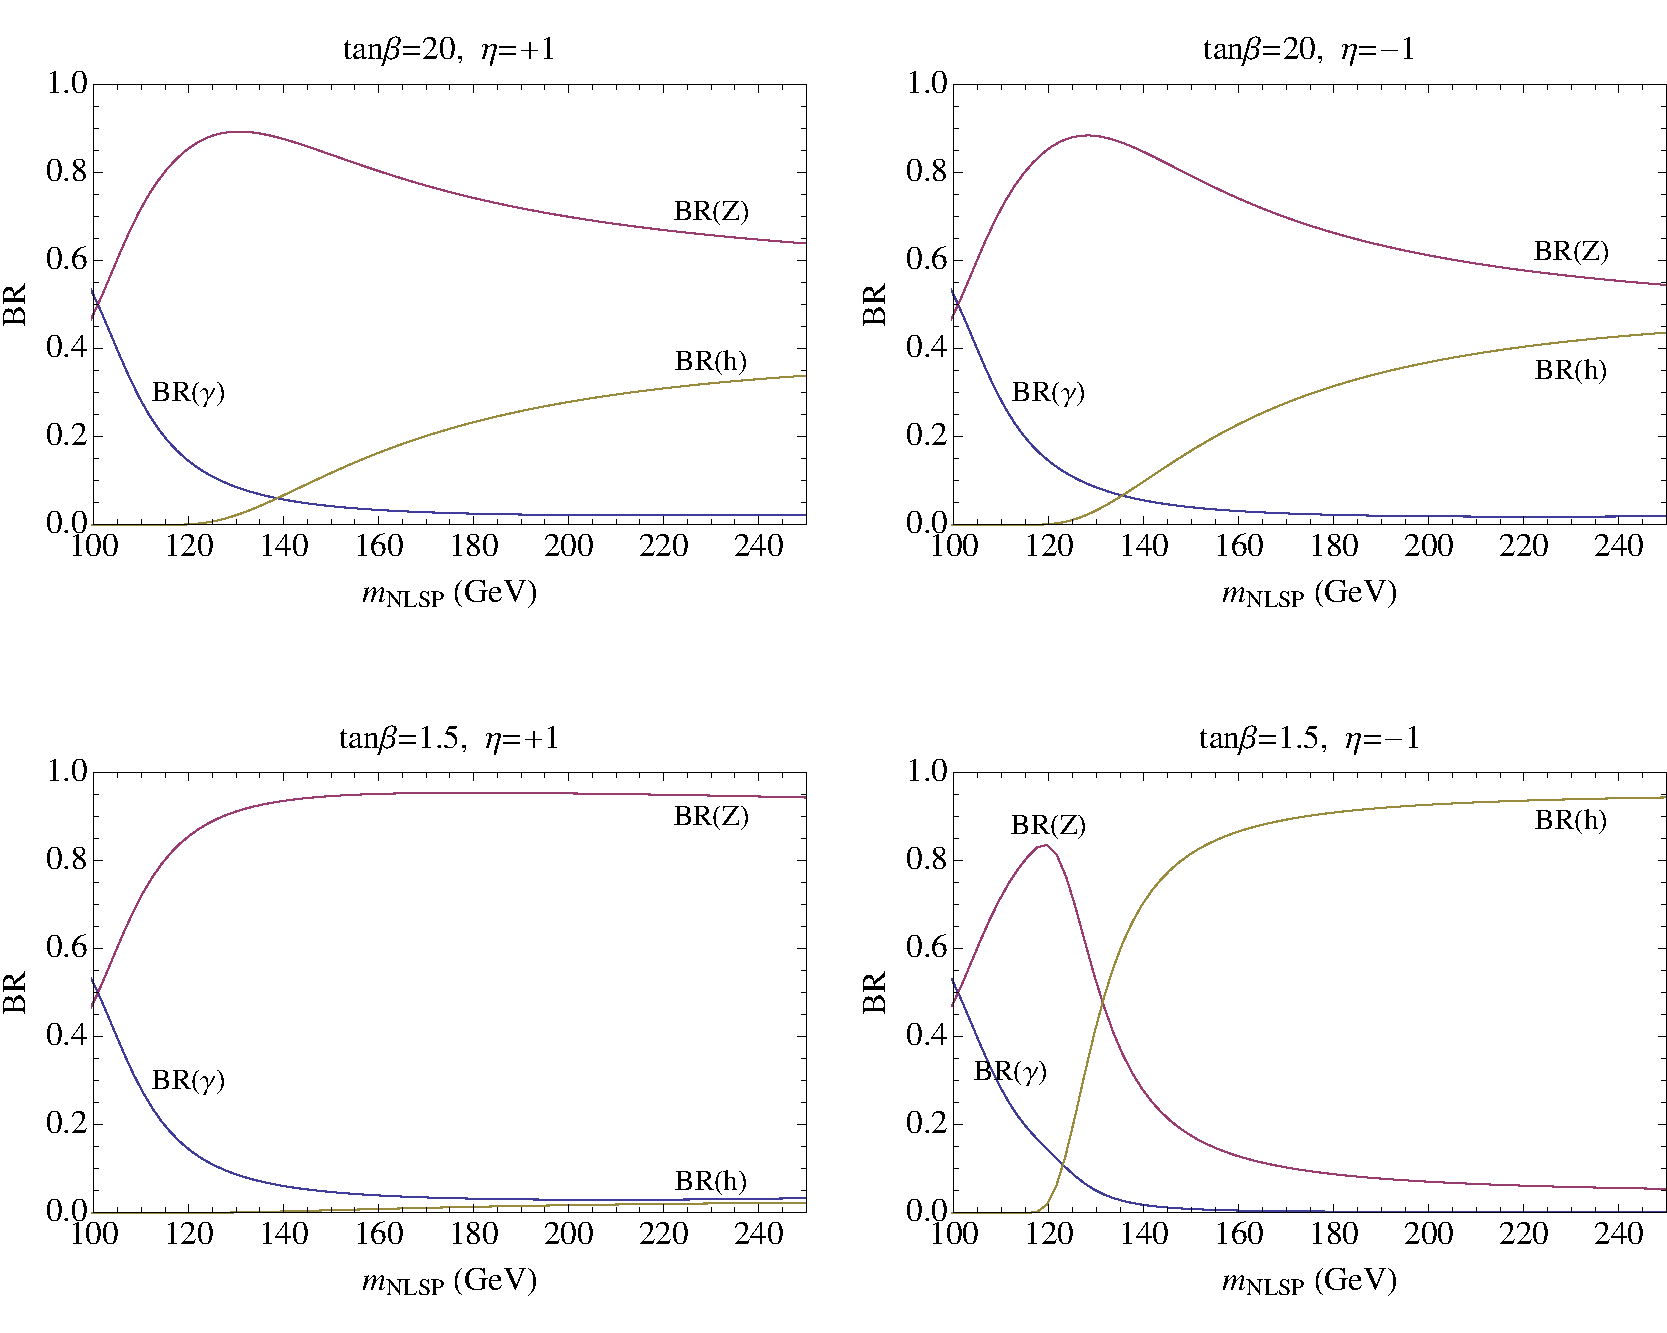
\includegraphics[width=0.95\textwidth]{figures/ewk_prod/varie/BRfracs}
\caption{Branching ratios of the higgsino NLSP to a photon, a $Z$ boson, and a Higgs boson, as a function of $m_{NLSP}$, for $\eta=\pm1$ and $\tan\beta=1.5,\,20$. In all the figures, $M_1=500$ GeV, $M_2=1000$ GeV, and $m_{h^0}=115$ GeV. Figure from Ref. \cite{Meade:2009qv}.}
\label{fig:higgsinoBR}
\end{figure}

The decay to photon is relevant only for very low \mhino, where the other decays are kinematically suppressed. 
Once all the kinematic decays are allowed, the \gls{br} is mostly to $Z$ boson or Higgs boson; 
the assumption of $B(\hino\rightarrow h \tilde{G}) = 100$\%, used to optimize this analysis, is 
realized in the case of relatively low $\tan \beta$ and $\eta = -1$.
Instead for low $\tan \beta$ and $\eta = +1$ the dominant decay is to a $Z$ boson, while for high 
$\tan \beta$ both $B(\hino\rightarrow h \tilde{G})$ and $B(\hino\rightarrow Z \tilde{G})$ tend to 
converge to the same value for high higgsino mass.
This motivates the interpretation of this analysis as a function of $B(\hino\rightarrow h \tilde{G})$, 
assuming $B(\hino\rightarrow h \tilde{G}) +B(\hino\rightarrow Z \tilde{G}) =1$, presented in Section \ref{sec:ewk:interp}.



%\section{Previous Limits}



\section{Discriminating variables}
\label{sec:ewk:sigbkg}

A key ingredient of the analysis is the reconstruction of the two Higgs bosons from the decay of the Higgsinos.
Since this analysis targets events where both Higgs bosons decay to a $b\bar{b}$ pair, the reconstruction starts 
from four jets, which are chosen according to an ordering that favors $b$-tagged jets over non-tagged jets,
and then orders based on \pt. Practically, this results in the following criteria:
\begin{itemize}
\item If there are exactly four $b$-tagged jets in the event, those are used.
\item If there are more than four $b$-tagged jets, the selected ones are the four $b$-tagged jets with highest \pt.
\item If there are less than four $b$-tagged jets, the selected ones are the $b$-tagged jets and the non-tagged jets with highest \pt.
\end{itemize} 

Once the four jets have been selected, they are grouped in two pairs, each one constituting a candidate Higgs bosons. 
Different algorithms to pair the jets have been tested, and the chosen one is based on minimizing the angular separation 
between the two jets associated to the same Higgs boson candidate. 
In particular, the permutation chosen is the one that minimizes:
\begin{equation}
\dRmax = \mathrm{max}(\Delta R(h_1), \Delta R(h_2)) \; ,
\end{equation}

\noindent where $\Delta R(h)$ is the distance in the $\eta-\phi$ space between the two jets from the same candidate.
This choice has a good efficiency in reconstructing the Higgs bosons in the signal, 
and at the same time avoids creating artificial peaks in the background in correspondence of the Higgs boson mass. 

Beside the variables described in Section \ref{sec:common_variables}, a few other discriminating variables particularly 
effective for this signal model are described below.

\subsubsection*{Candidate Higgs bosons}

The invariant mass of the two Higgs boson candidates built following the procedure outlined in Section \ref{sec:ewk:higgsreco} 
are used as discriminating variable. In particular, we refer to m($h_1$) and m($h_2$) respectively for the mass of the Higgs candidate with 
the leading and subleading mass.

The variable \dRmax, defined in the previous section, is used to choose the pairing of the jets while reconstructing 
the Higgs boson candidates but also as a discriminating variable to separate signal and background. 

\subsubsection*{Modified effective mass}

In the signal model, only four jets come from the hard scattering process, and are therefore expected to be more energetic than the 
remaining jets in the event. Therefore the \meff definition is modified to include only the jets that are selected 
as originating from a Higgs boson; the modified definition is therefore:
\begin{equation}
\meffb = \sum_{i=1,..,4} {\pt}^{j_i} + \met
\end{equation}
\noindent where the sum runs over the jets selected according to the ordering procedure presented in Section \ref{sec:ewk:higgsreco}. 


The variables defined above, together with the ones defined in Section \ref{sec:common_variables} 
allow identifying a region of the phase space that is enriched in signal events. 
This study is performed after selecting events with high \met ($> 200$ GeV), at least four signal jets and, least three $b$-tagged jets, zero signal leptons and \dphimin $>0.4$.

Figures \ref{fig:ewk:sig:1} and \ref{fig:ewk:sig:2}  show the distribution of the main kinematic variables for 
the sum of the \gls{sm} backgrounds and for different signal samples after these selections.
Figures \ref{fig:ewk:sig:mass_h1_min_dR} and \ref{fig:ewk:sig:mass_h2_min_dR} show the distribution of the mass of the Higgs 
candidate with the leading and subleading mass respectively. As can be appreciated, the distribution peaks at values around the Higgs mass for 
signals, while it is flatter for background. 
The distribution of \dRmax is shown in Figure \ref{fig:ewk:sig:dRmax_dR}. This variable assumes in general a lower value for 
signal events, in particular for the high-mass signals, where the Higgs bosons are produced with higher \pt and thus have 
more collimated decay products. Signal events also tend to have a lower number of signal jets, as can be observed in Figure 
\ref{fig:ewk:sig:jets_n}, and they occupy mostly the bins with three and four $b$-jets in the 
distribution of \nbjet (Figure \ref{fig:ewk:sig:bjets_n}). 
The \met distribution, shown in Figure \ref{fig:ewk:sig:met}, displays the expected features: while signals with low-mass Higgsinos 
have low \met values, the distribution tends to assume increasingly high values with the increase of the Higgsino mass. 
A similar feature is shown in Figures \ref{fig:ewk:sig:meff_4bj} and \ref{fig:ewk:sig:mTb_min} for the \meffb and \mtb distributions respectively: 
the higher the Higgsino mass in the signal, the more signal events differ from background events. 
While on the one hand this makes it easier to separate them from the \gls{sm} background, on the other hand the increase in signal mass 
implies a decrease in production cross-section, which will be the limiting factor in sensitivity to high-mass signals. 

\begin{figure*}[htbp]
\centering 
\subfigure[m($h_1$)]{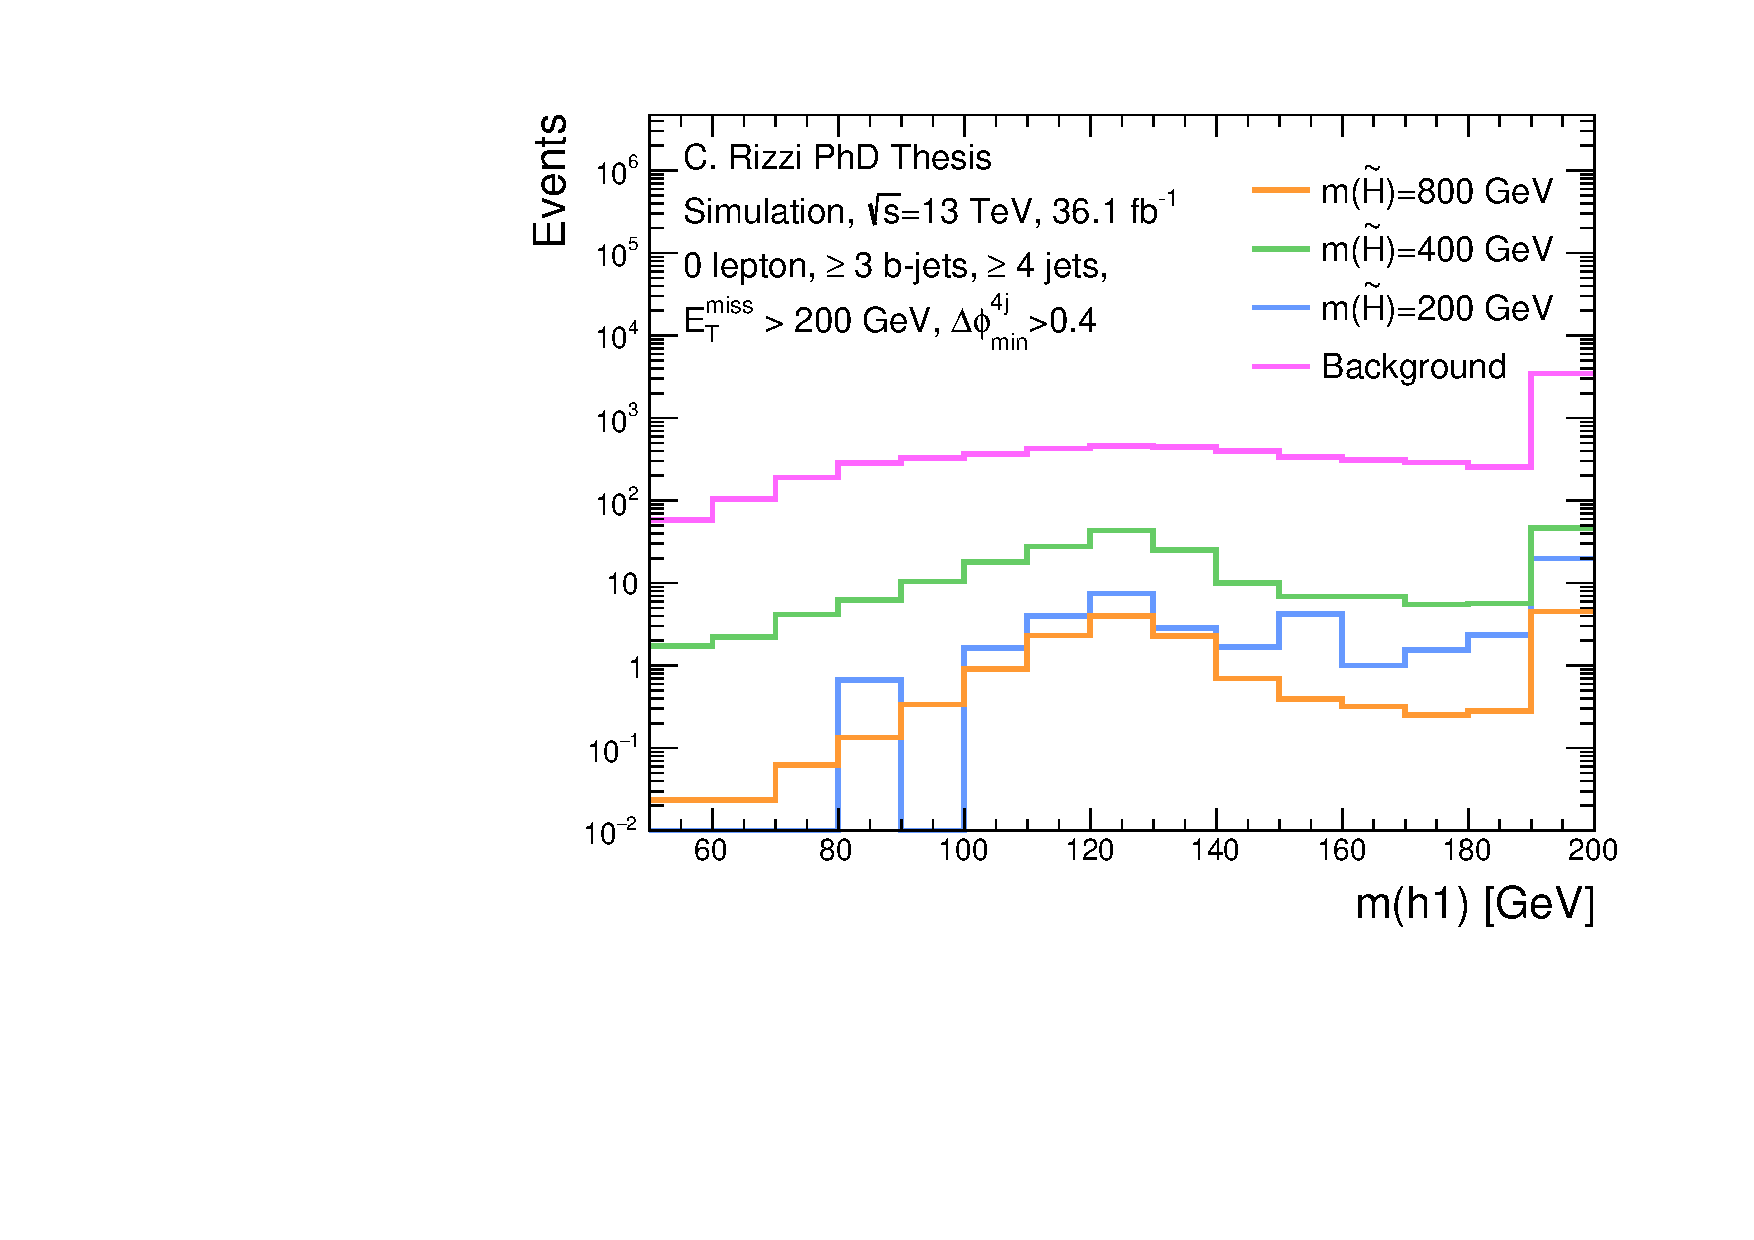
\includegraphics[width=0.48\textwidth]{figures/ewk_prod/sig_bkg/hh_compare_mass_h1_min_dR.pdf}\label{fig:ewk:sig:mass_h1_min_dR}}
\subfigure[m($h_2$)]{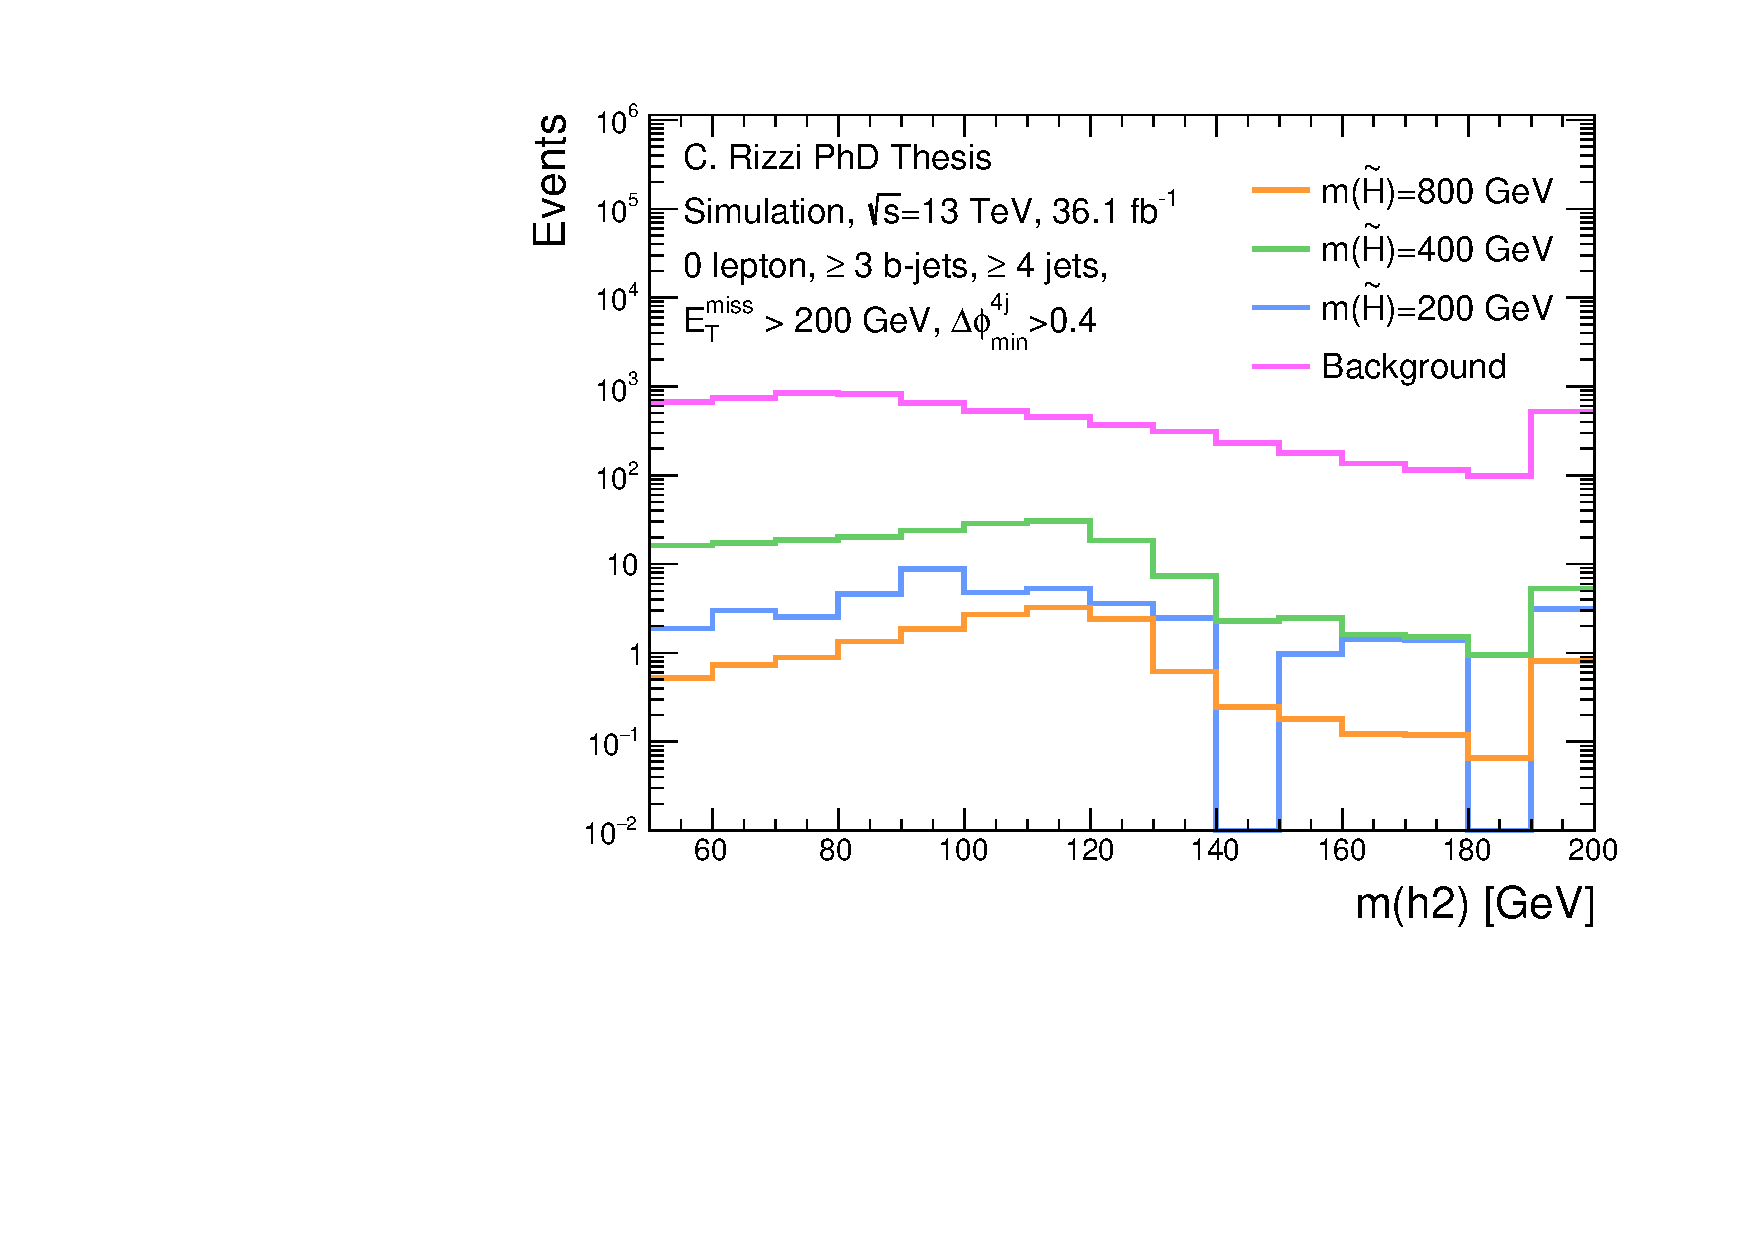
\includegraphics[width=0.48\textwidth]{figures/ewk_prod/sig_bkg/hh_compare_mass_h2_min_dR.pdf}\label{fig:ewk:sig:mass_h2_min_dR}} \\
\subfigure[\dRmax]{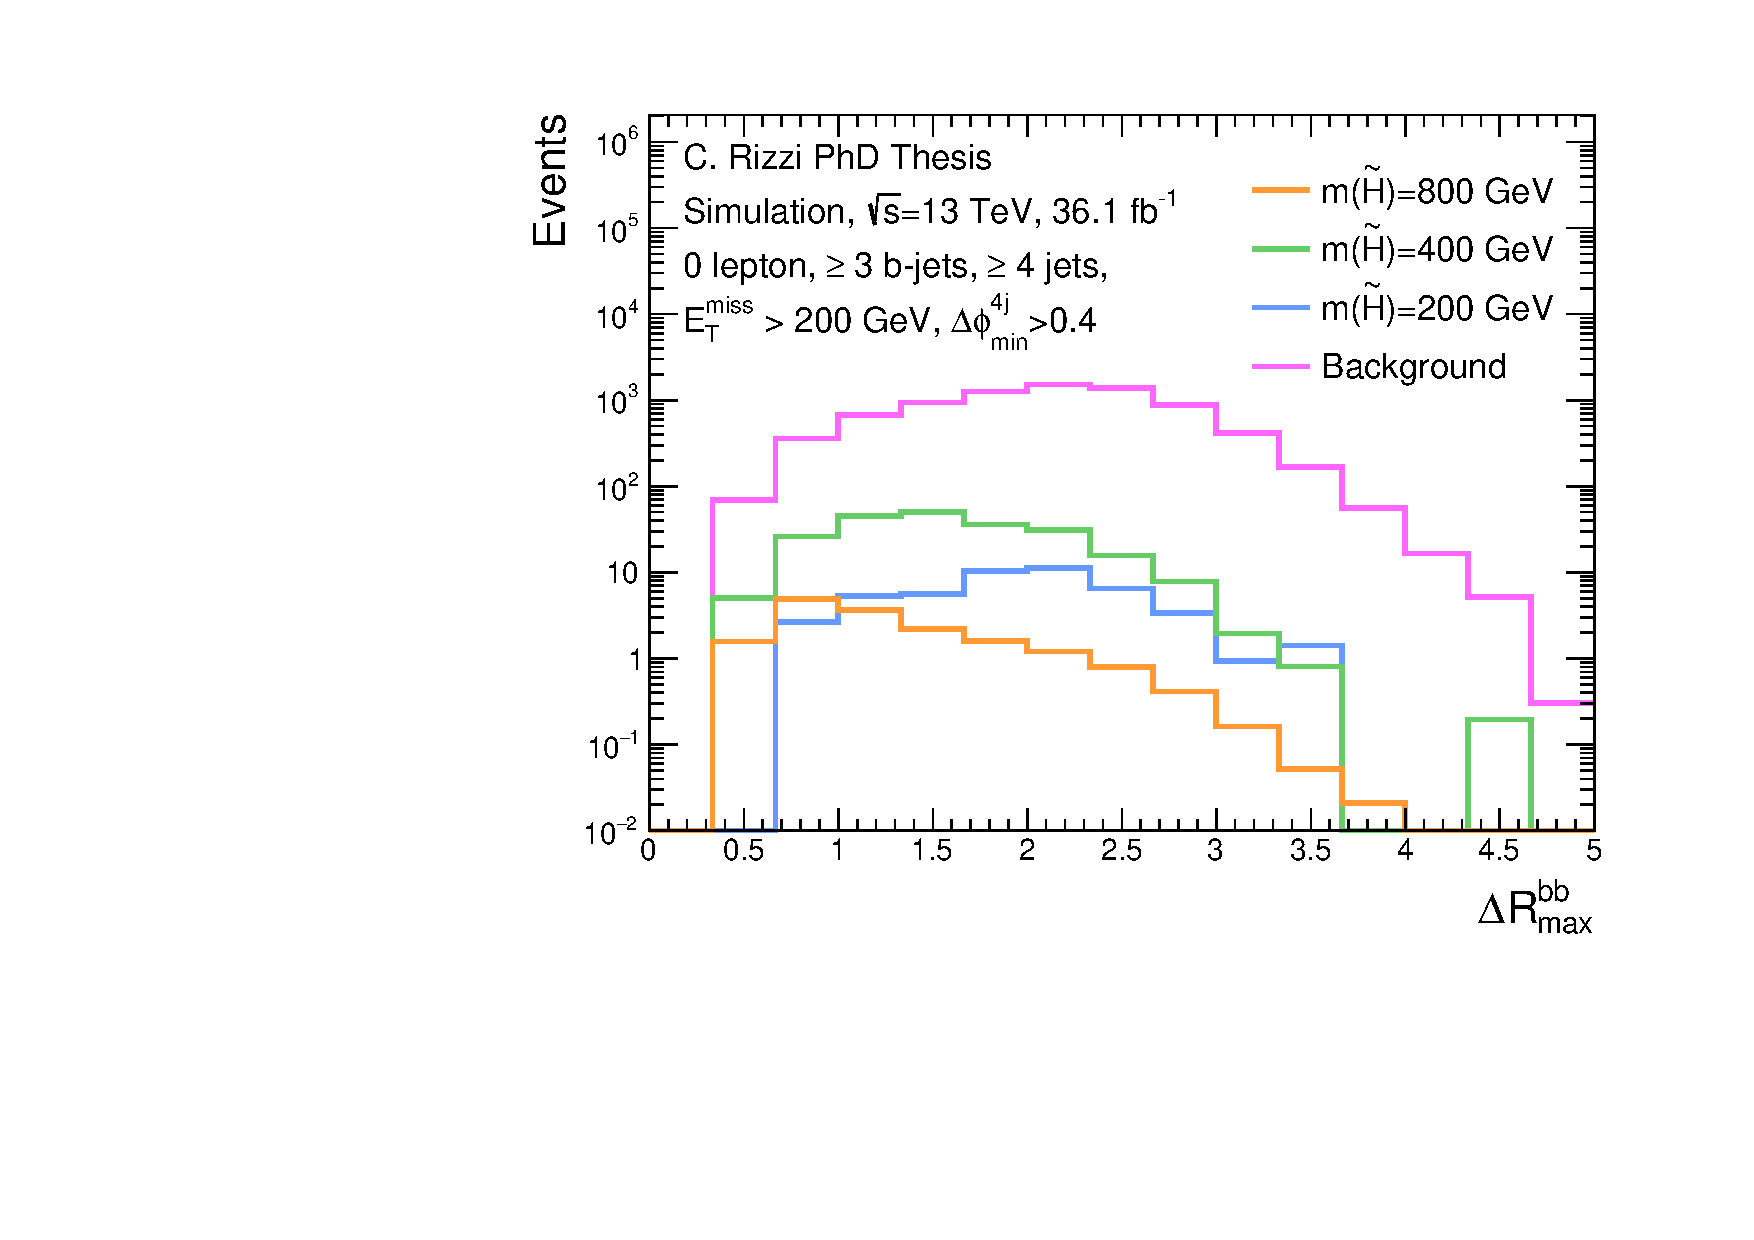
\includegraphics[width=0.48\textwidth]{figures/ewk_prod/sig_bkg/hh_compare_dRmax_dR.pdf}\label{fig:ewk:sig:dRmax_dR}}
\subfigure[\meffb]{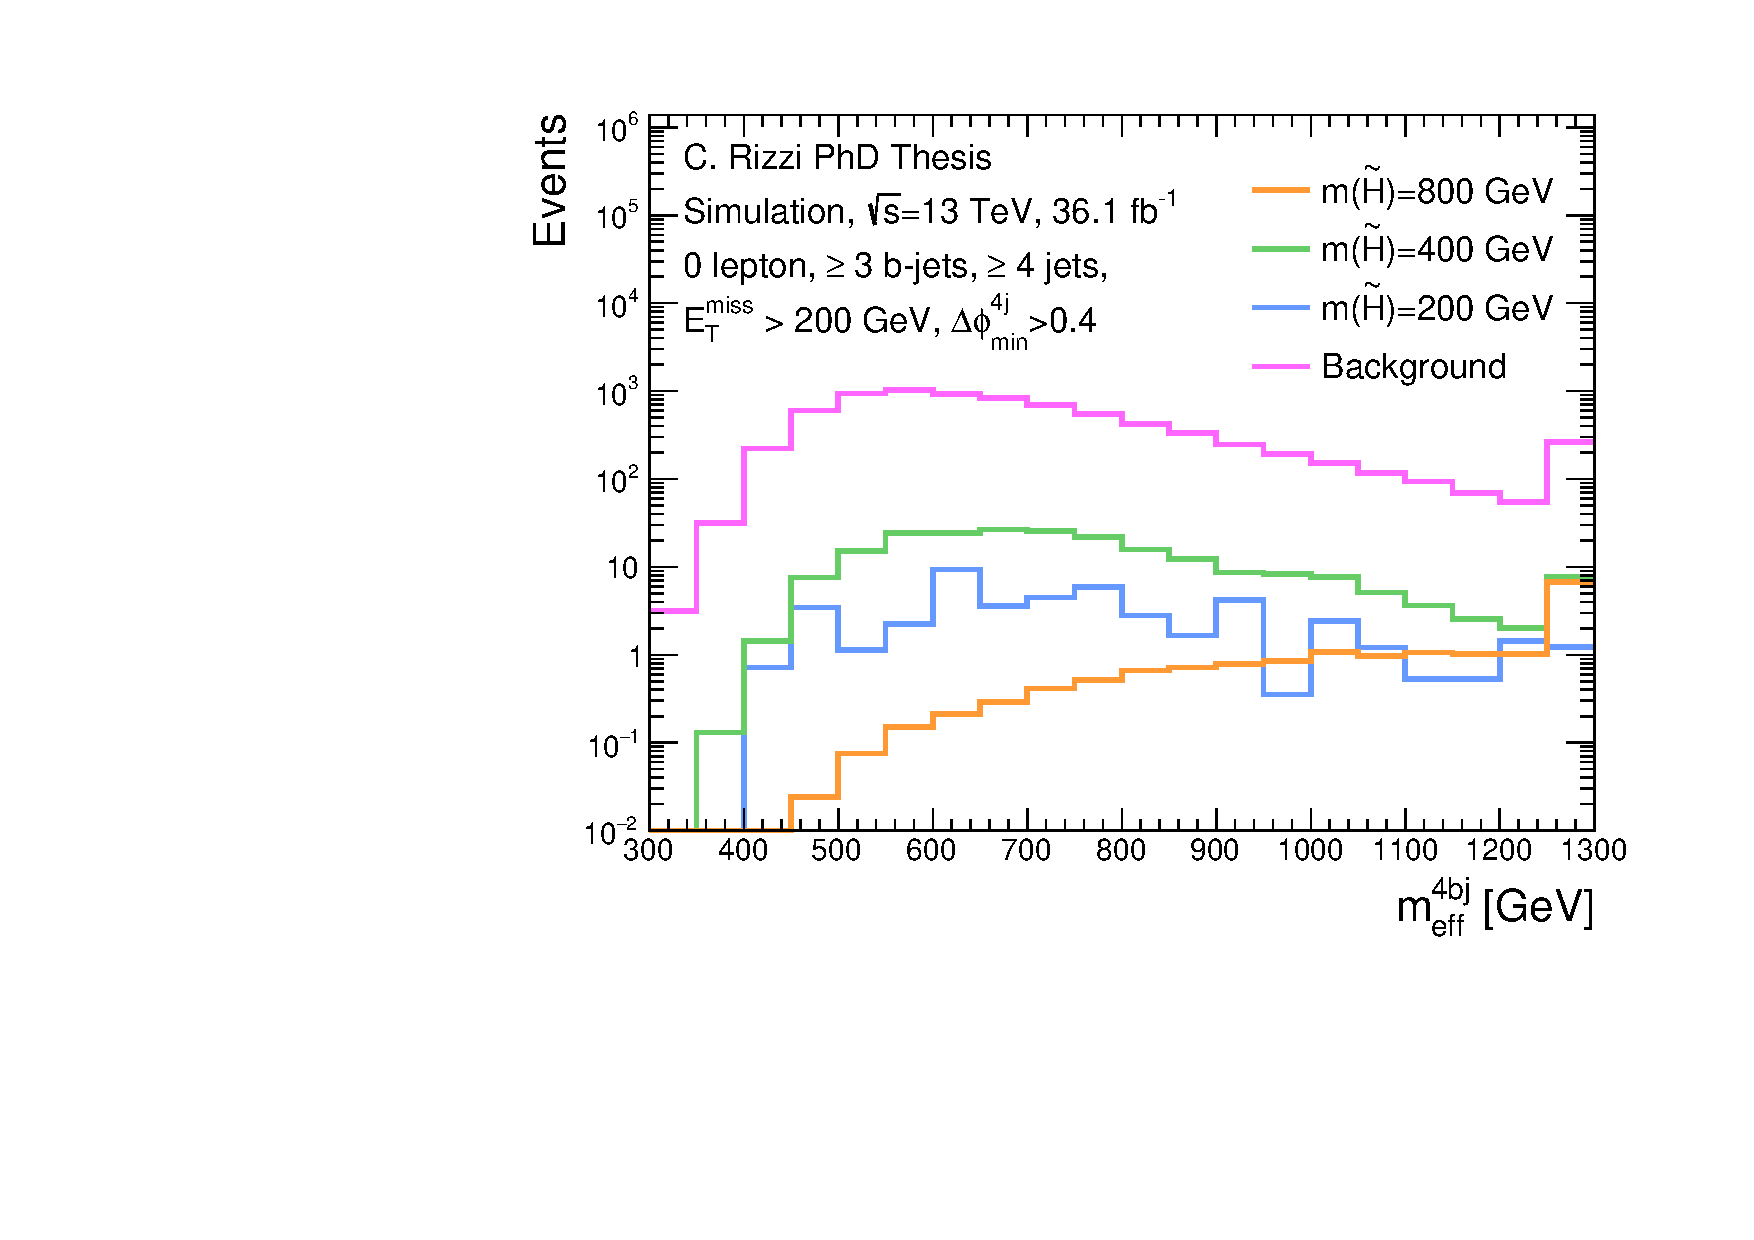
\includegraphics[width=0.48\textwidth]{figures/ewk_prod/sig_bkg/hh_compare_meff_4bj.pdf}\label{fig:ewk:sig:meff_4bj}}
\caption{Distribution of  the main kinematic variables in background and signal events after the selections described in the text.}
\label{fig:ewk:sig:1}
\end{figure*}

\begin{figure*}[htbp]
\centering
\subfigure[\njet]{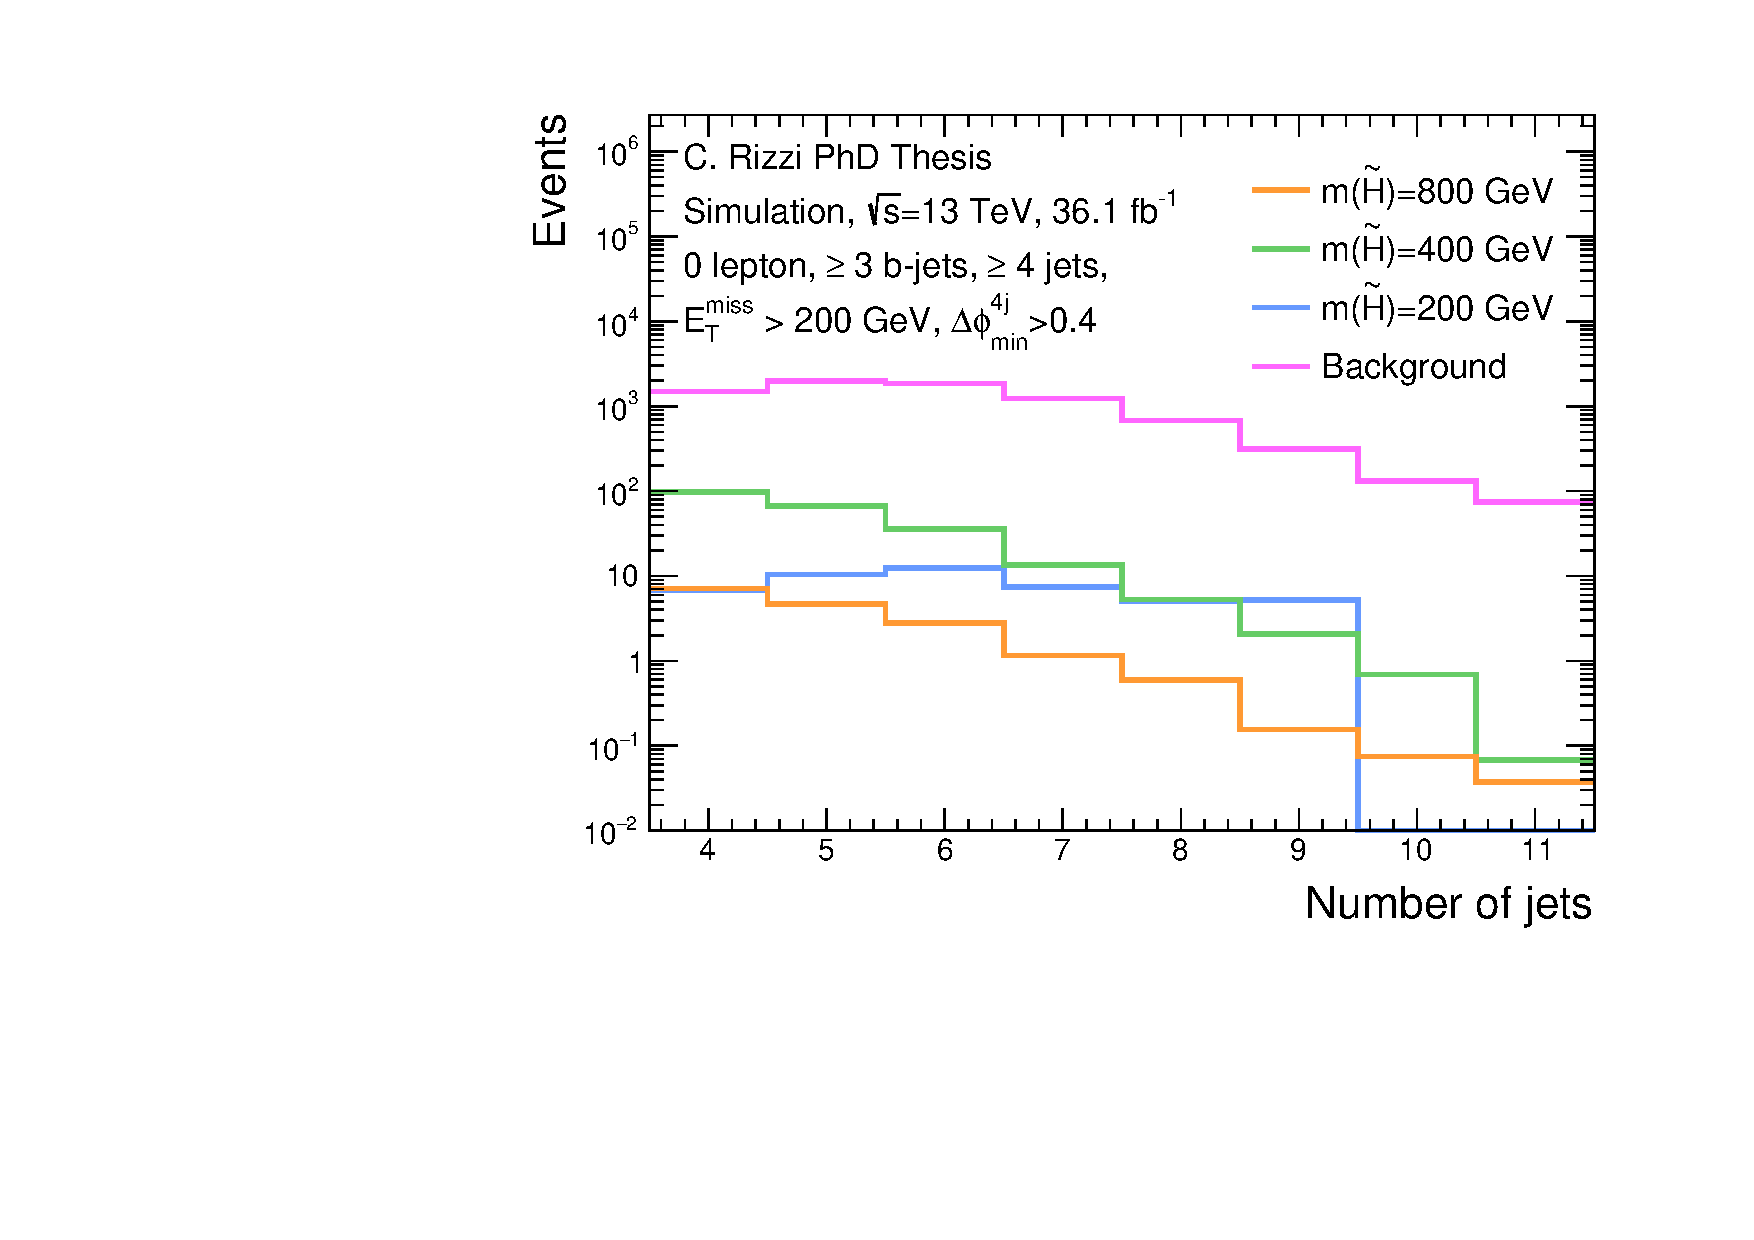
\includegraphics[width=0.48\textwidth]{figures/ewk_prod/sig_bkg/hh_compare_jets_n.pdf}\label{fig:ewk:sig:jets_n}}
\subfigure[\nbjet]{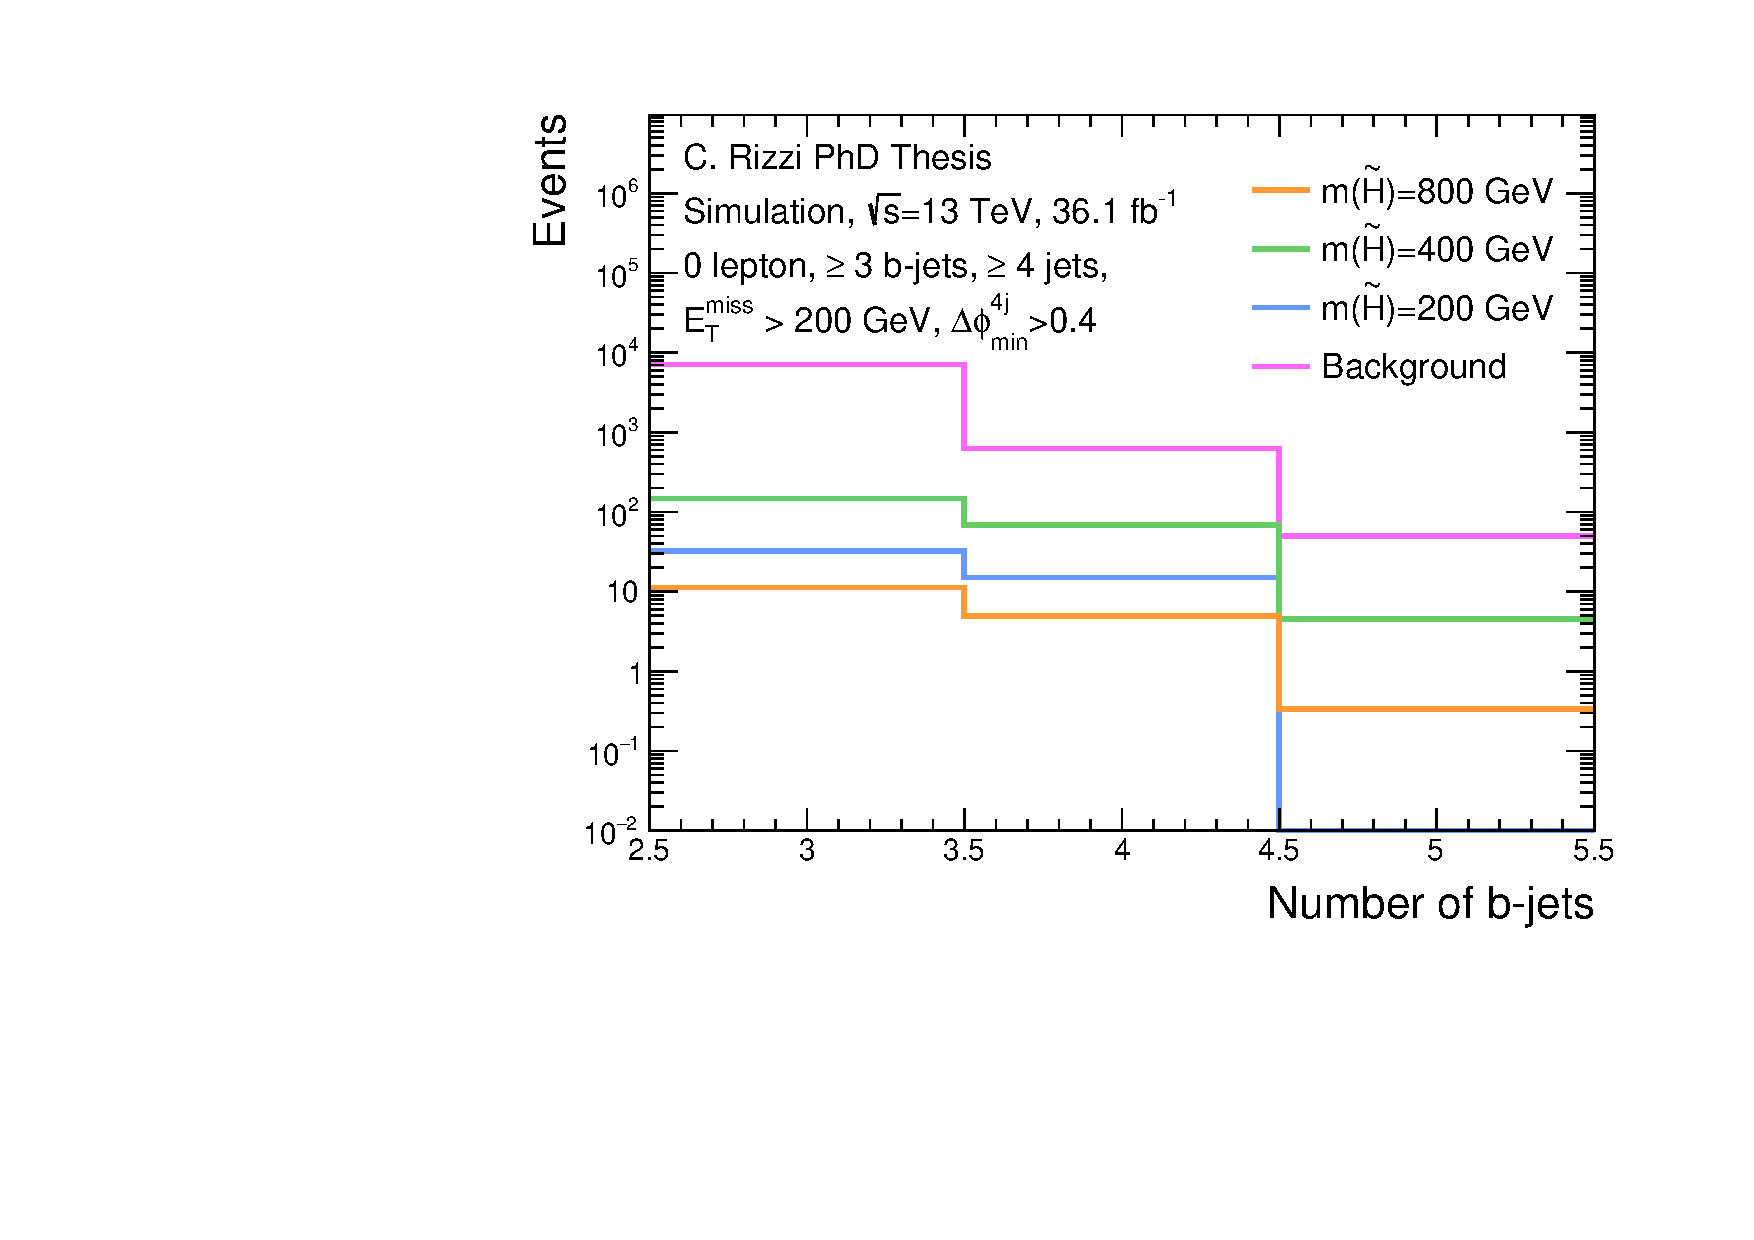
\includegraphics[width=0.48\textwidth]{figures/ewk_prod/sig_bkg/hh_compare_bjets_n.pdf}\label{fig:ewk:sig:bjets_n}}\\
\subfigure[\met]{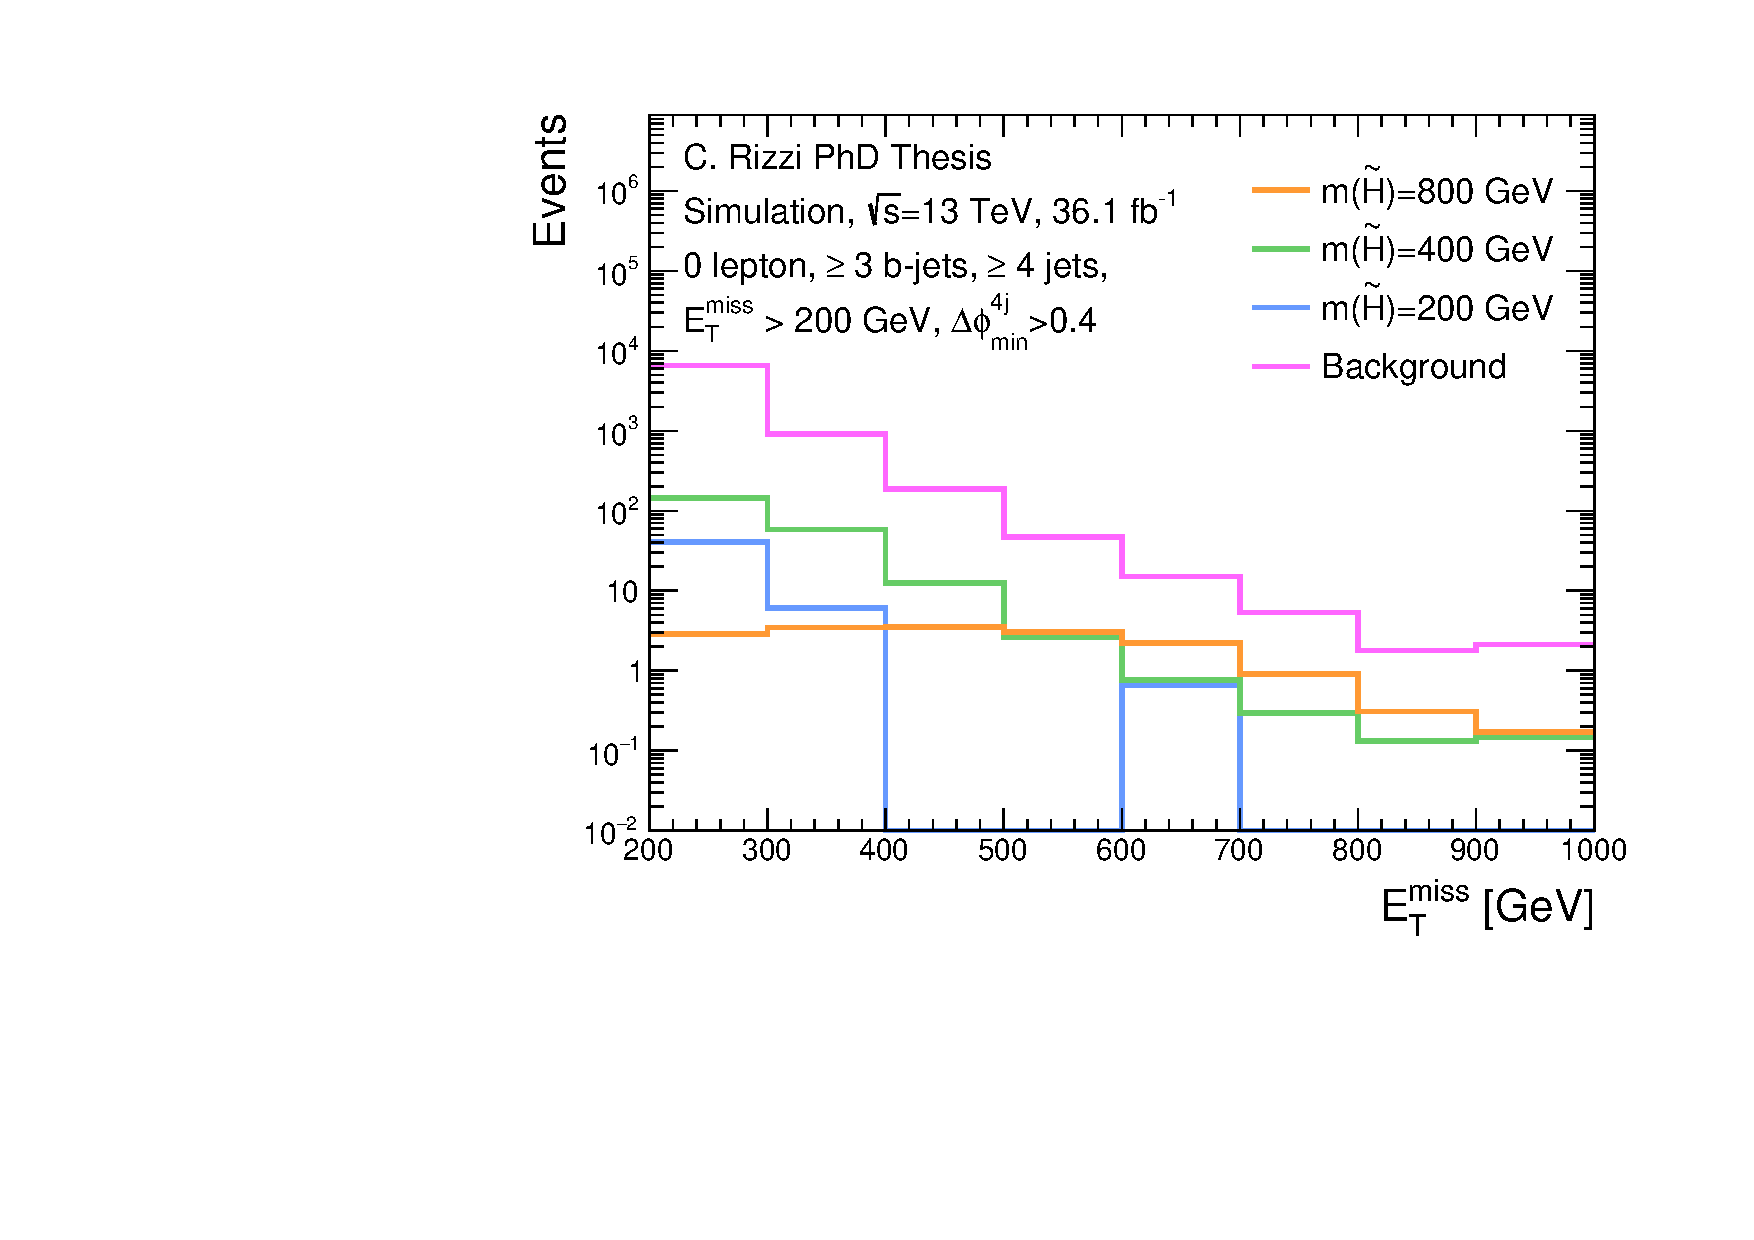
\includegraphics[width=0.48\textwidth]{figures/ewk_prod/sig_bkg/hh_compare_met.pdf}\label{fig:ewk:sig:met}}
\subfigure[\mtb]{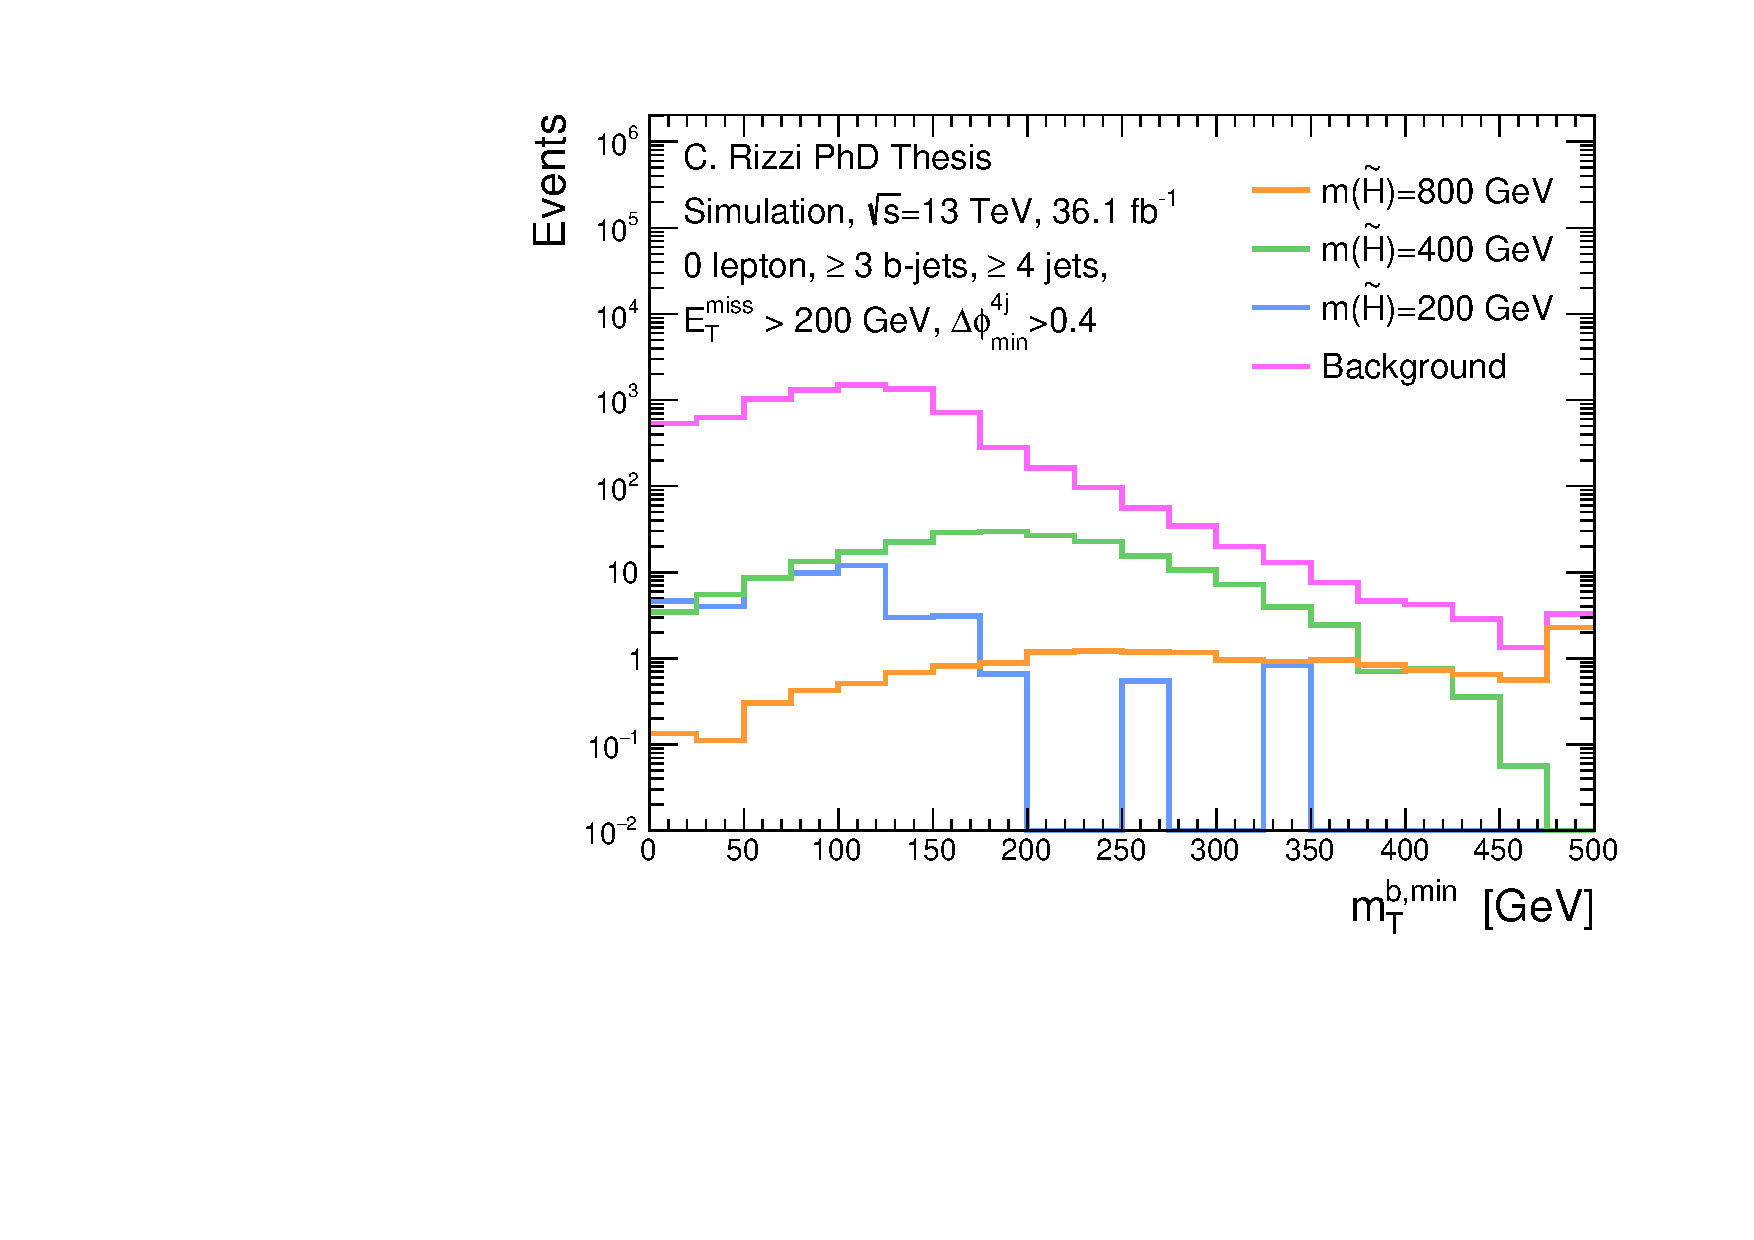
\includegraphics[width=0.48\textwidth]{figures/ewk_prod/sig_bkg/hh_compare_mTb_min.pdf}\label{fig:ewk:sig:mTb_min}}
\caption{Distribution of  the main kinematic variables in background and signal events after the selections described in the text.}
\label{fig:ewk:sig:2}
\end{figure*}

\FloatBarrier

\section{Signal regions}

This section describes the optimization of the \glspl{sr}. 
The high branching ratio of the h$\rightarrow$bb (58\%) makes the $\geq$3b channel the most promising to look for signal models 
in which both $\ninoone$ decay to h+$\gravino$. 
Therefore, the analysis selection are optimized to maximize the expected sensitivity to signals leading to $hh+\met$ 
and all the \glspl{sr} require both boson candidates to have masses compatible with the Higgs mass (the specific mass range is chosen during the optimization). 
%The target signal model is shown in Figure \ref{fig:opt_sighh4b}.

\subsection{Multi-bin regions}
\label{sec:ewk:multibin}

The optimization of the multi-bin \glspl{sr} aims at constructing several orthogonal \glspl{sr}, that can be combined in a fit. 
The general strategy adopted follows these steps:
\begin{enumerate}
\item A first variable (var$_1$) is chosen to define a coarse binning. 
    This variable should provide both a good signal-to-background discrimination and discrimination between signal 
    with different Higgsino masses.
\item For each of these bins in var$_1$, a \gls{cr} is defined to normalize the \ttbar background in a kinematic regime close to the corresponding \gls{sr}.
\item Each bin based on var$_1$ is further split based on a second variable, var$_2$ (in this case all the bins based on the second variable share the same \gls{cr}).
\item The selections on the remaining kinematic variables are optimized independently in each var$_1$ bin (i.e. all the regions sharing the same 
\gls{cr} have the same selections on all the variables except var$_2$).
\end{enumerate}

\noindent As described above, var$_1$ must be able to provide at the same time a good separation between signal and background 
and a good separation between signals with different \hino masses. 
The latter is necessary in order to be able to optimize each bin in var$_1$ based on a different signal mass, 
providing in the end a good sensitivity to the entire mass spectrum. 
In order to understand which variable works best for this scope, the separation algorithm provided by the TMVA toolkit \footnote{TMVA is a toolkit designed for multivariate analyses, this in not the case here: it's only used as a quick way to access the discrimination power of the individual variables.} \cite{Hocker:2007ht} is used, defined as:

\begin{equation}
          \mathrm{separation} = \frac{1}{2} \int\frac{\left(f_s(x) - f_b(x)\right)^2}{f_s(x) + f_b(x)} dx \; , 
\label{eq:separation}
\end{equation}
\noindent where $f_s$ and $f_b$ are the signal and background \glspl{pdf} of $x$. 

The separation provided by the most promising analysis variables between background and 
signals with m(\hino)=300, 500 and 800 GeV is shown in Figure \ref{fig:ewk:separation}.
It is possible to see that \meffb is the best variable for our requirements (even if there are individual bins where this is not the case). 

\begin{figure}[htpb]
\begin{center}
%\subfigure[]{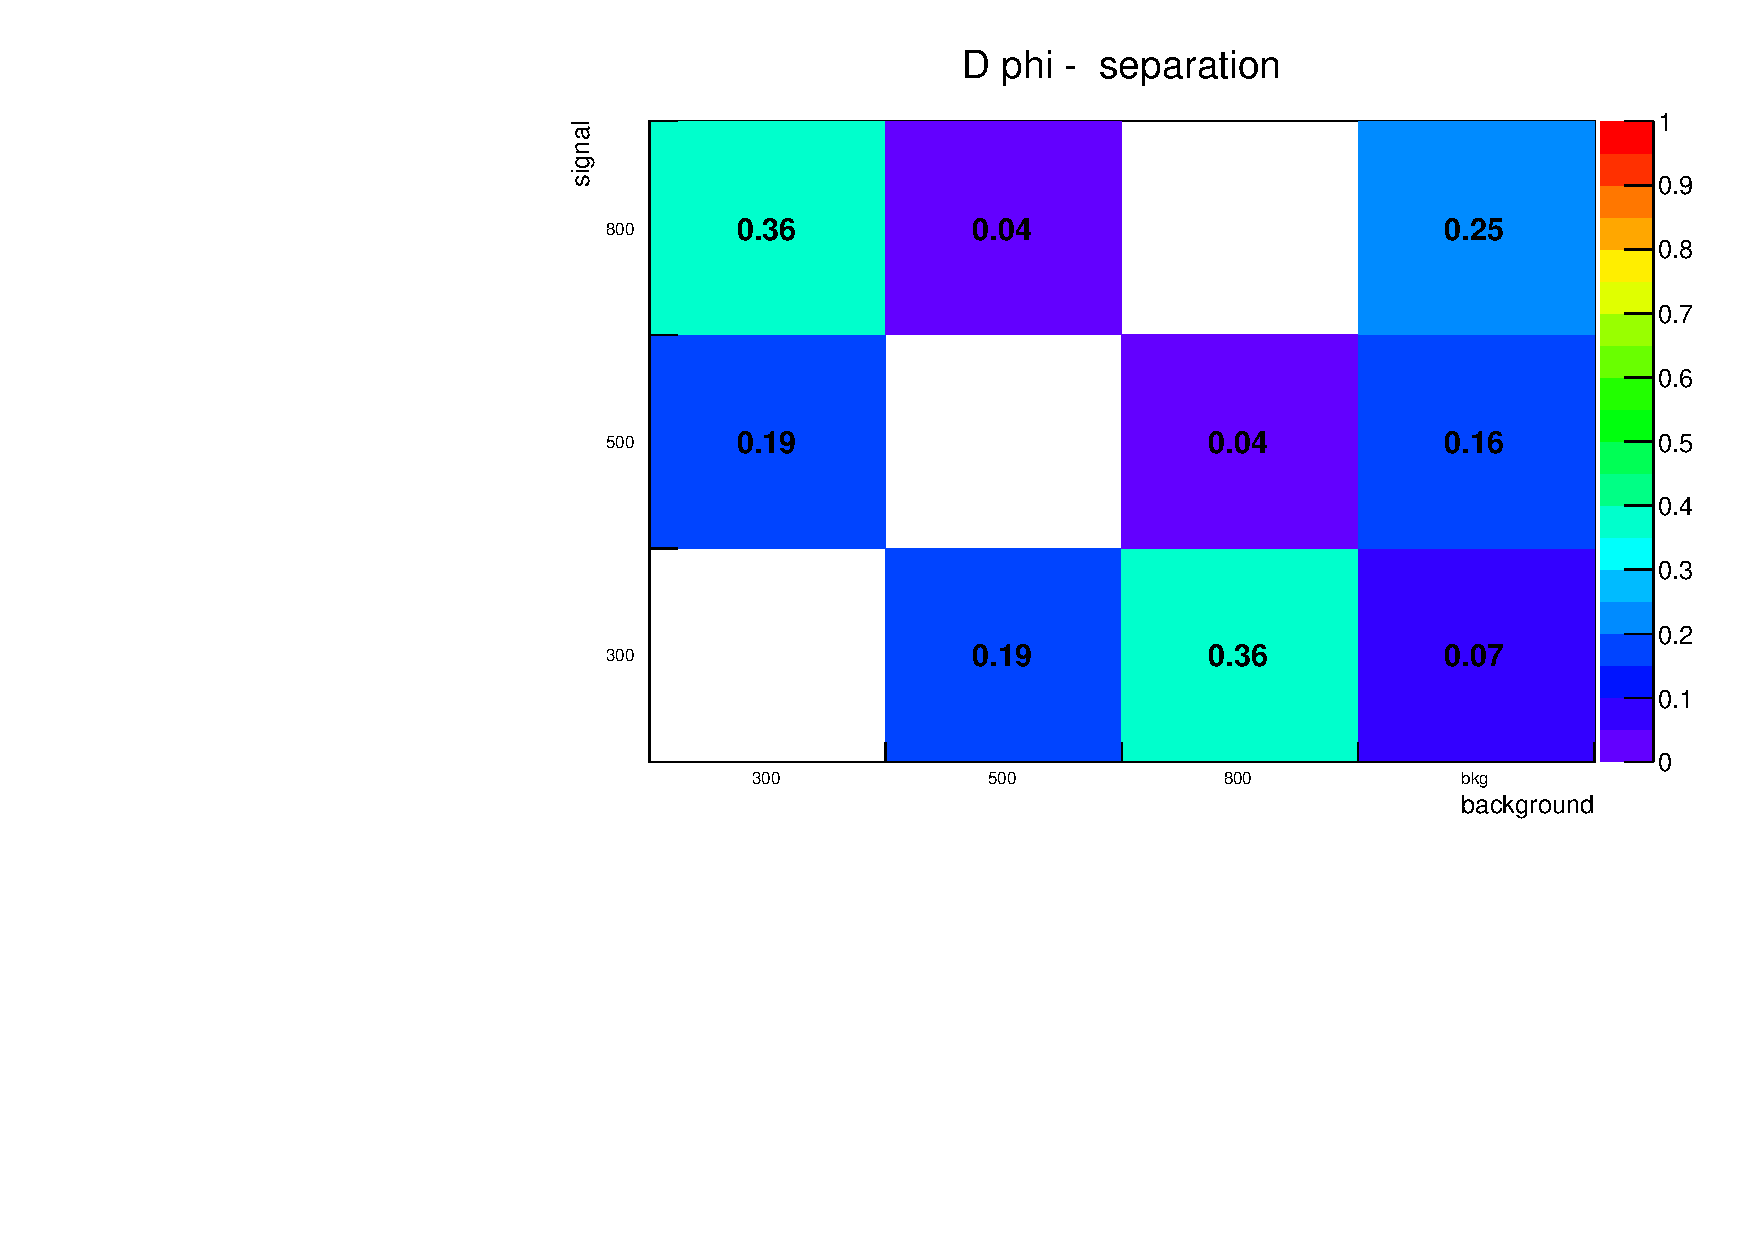
\includegraphics[width=0.43\textwidth]{figures/ewk_prod/separation/saparation_Dphi.pdf}}
\subfigure[]{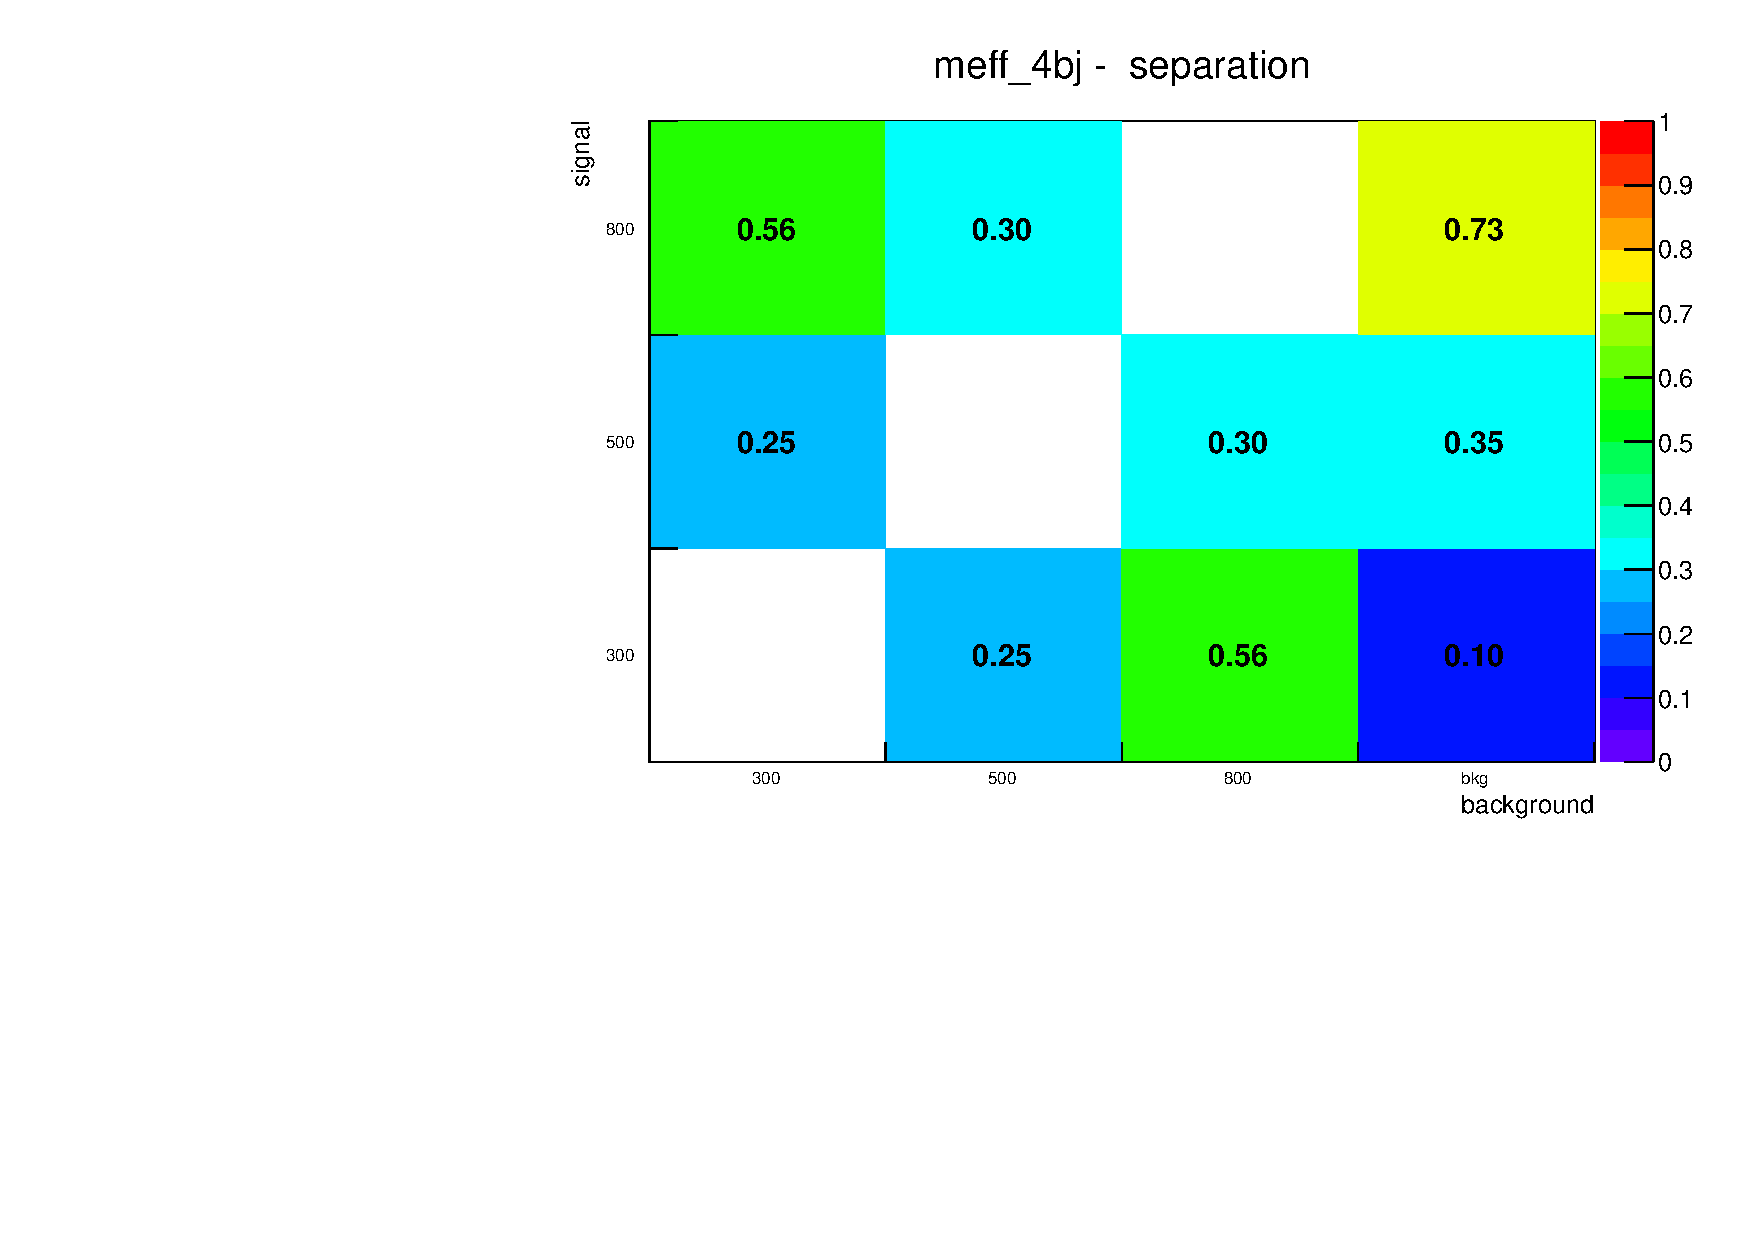
\includegraphics[width=0.43\textwidth]{figures/ewk_prod/separation/saparation_meff_4bj.pdf}}
\subfigure[]{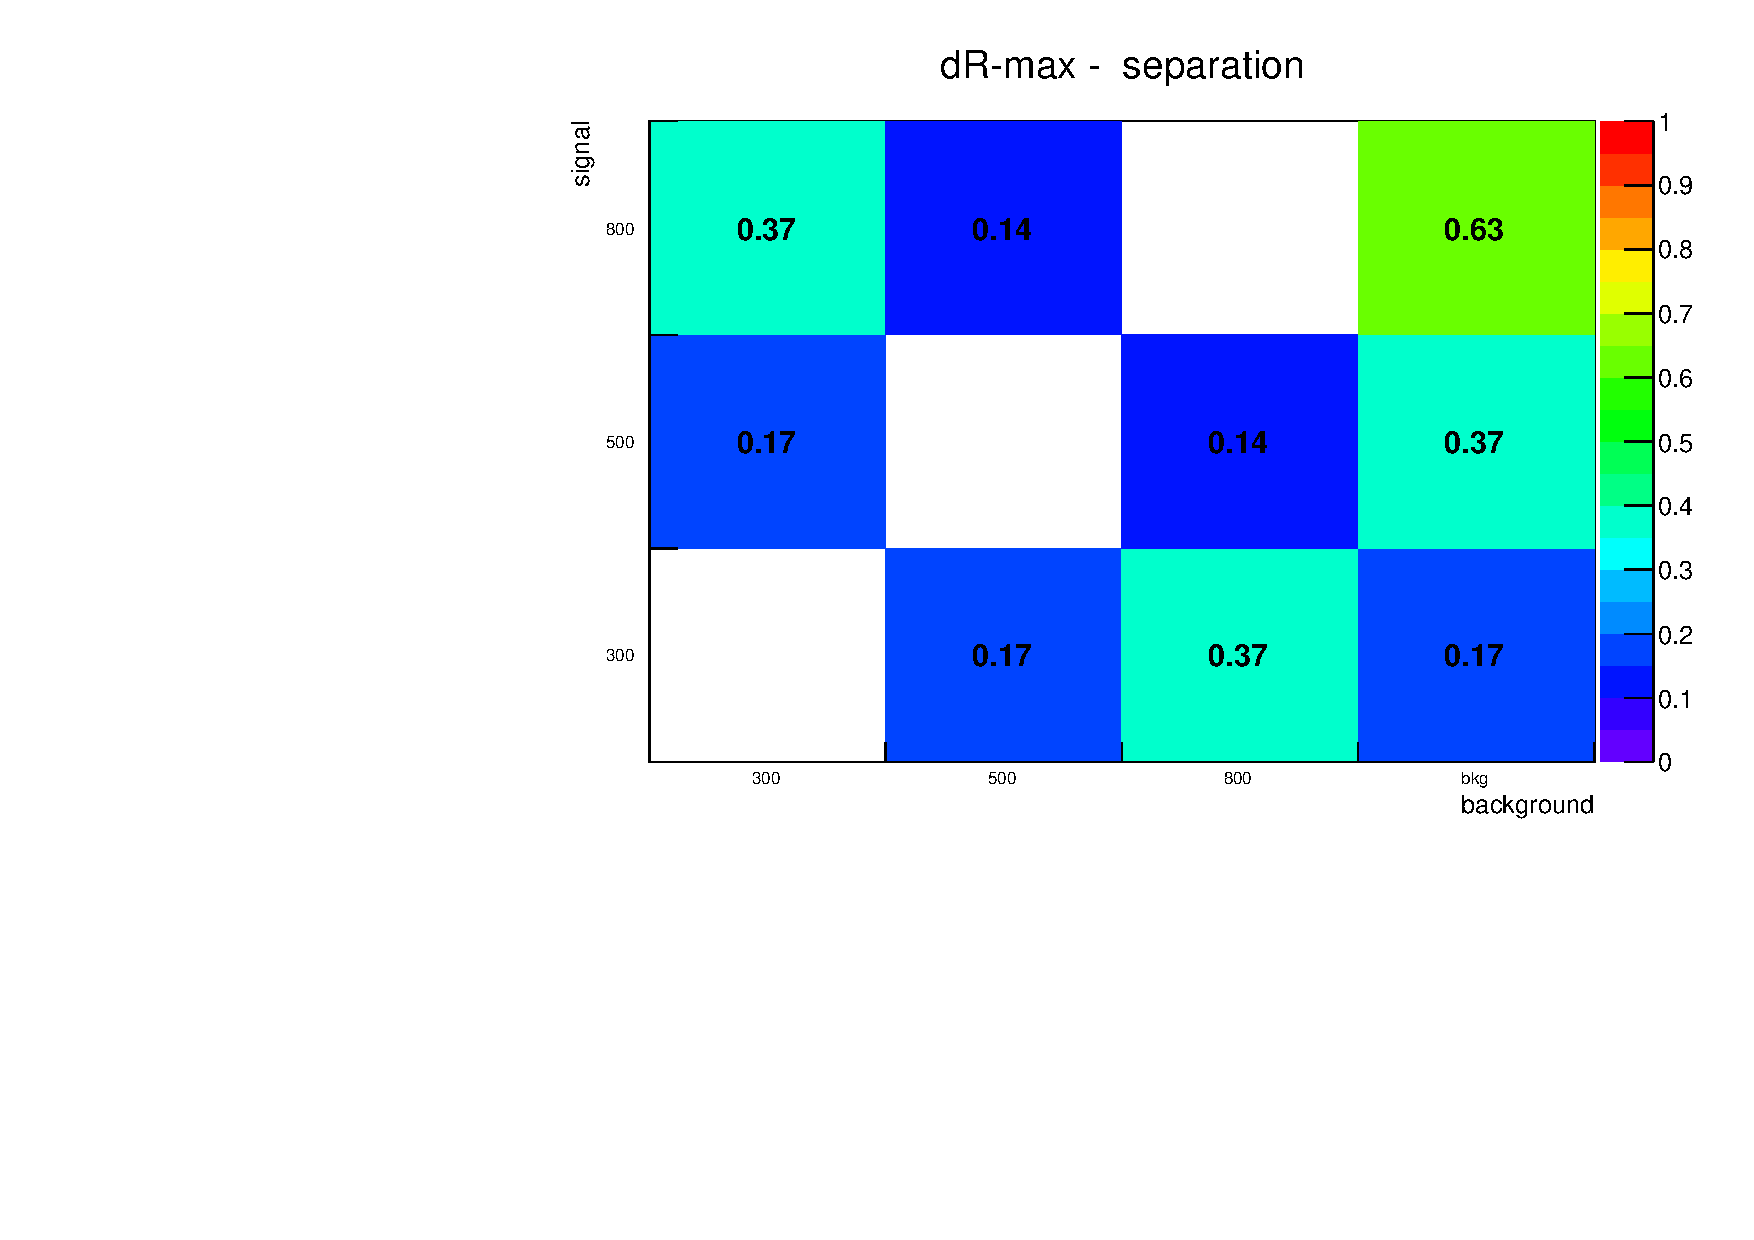
\includegraphics[width=0.43\textwidth]{figures/ewk_prod/separation/saparation_dR_max.pdf}}\\
\subfigure[]{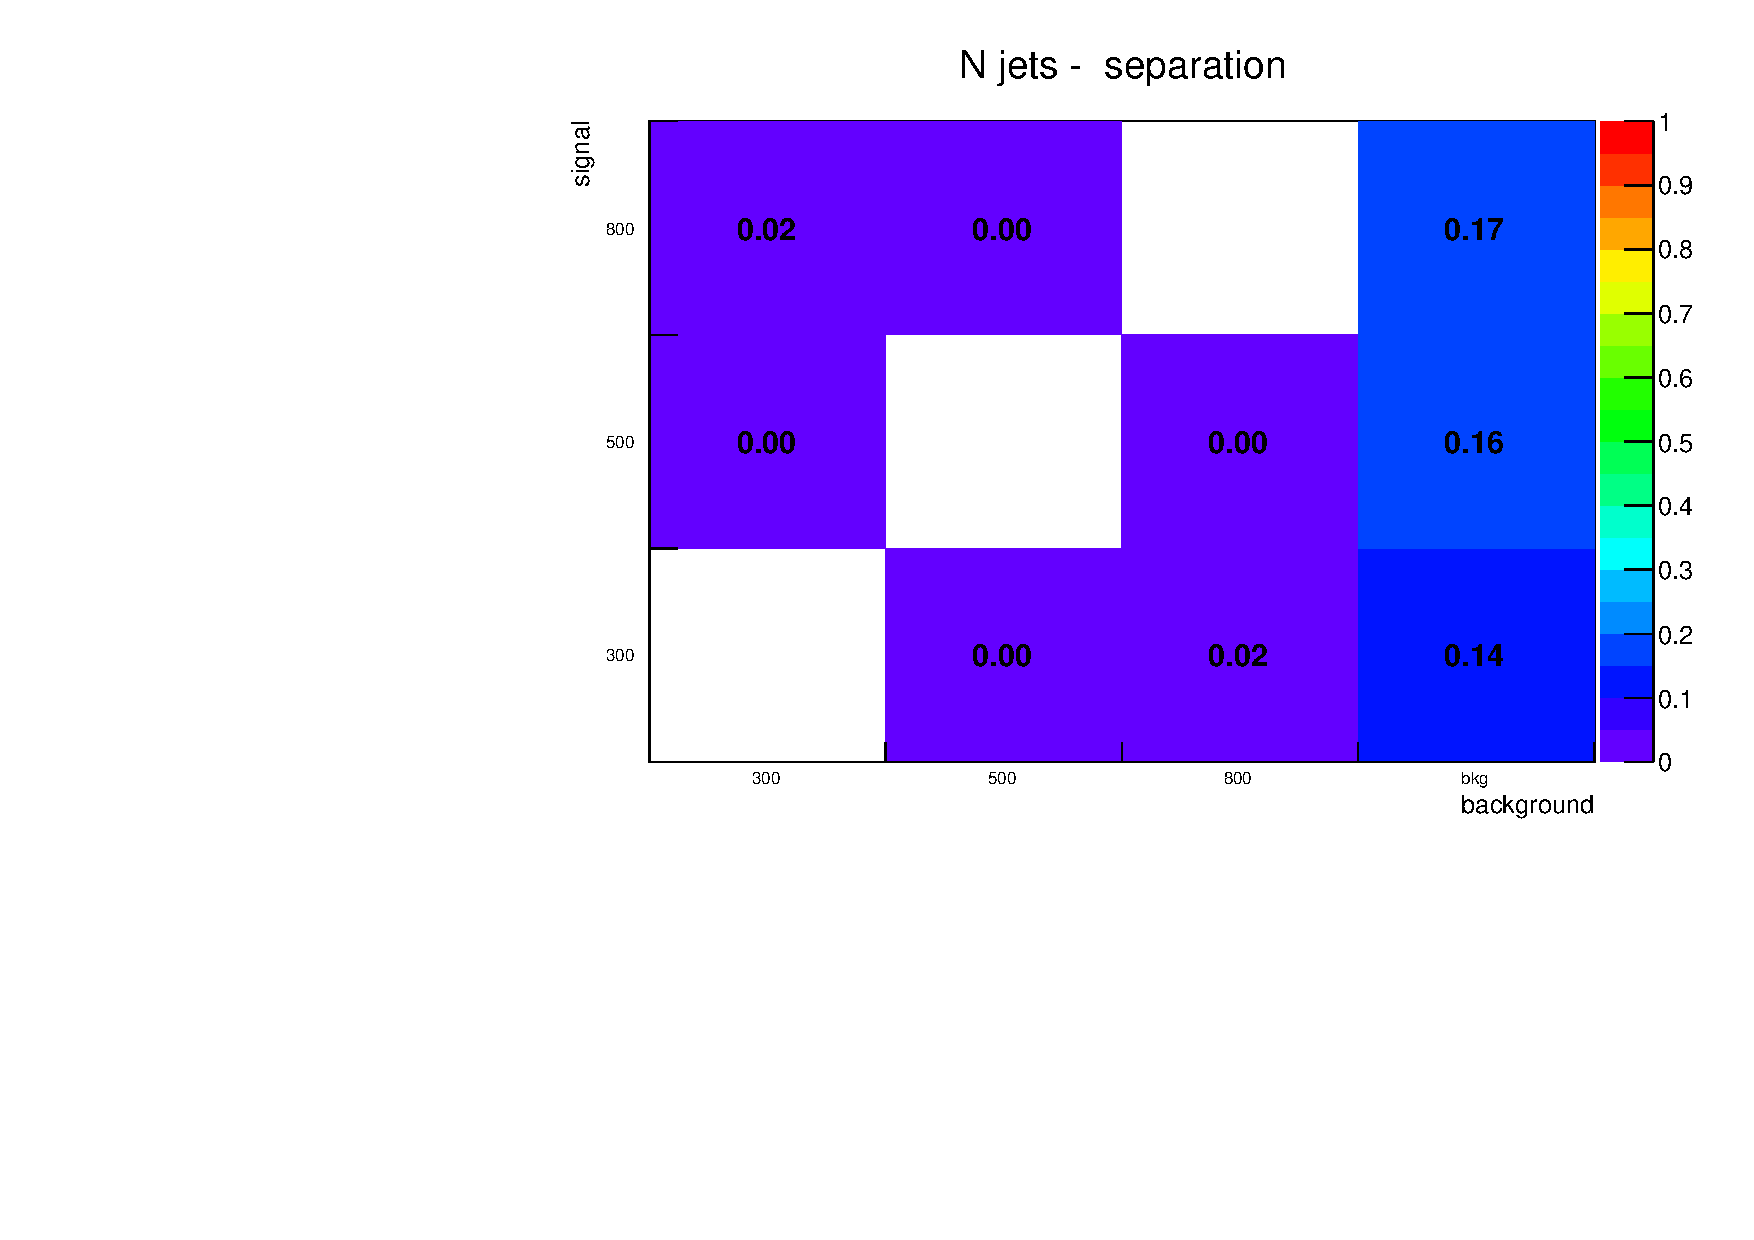
\includegraphics[width=0.43\textwidth]{figures/ewk_prod/separation/saparation_Njets.pdf}}
\subfigure[]{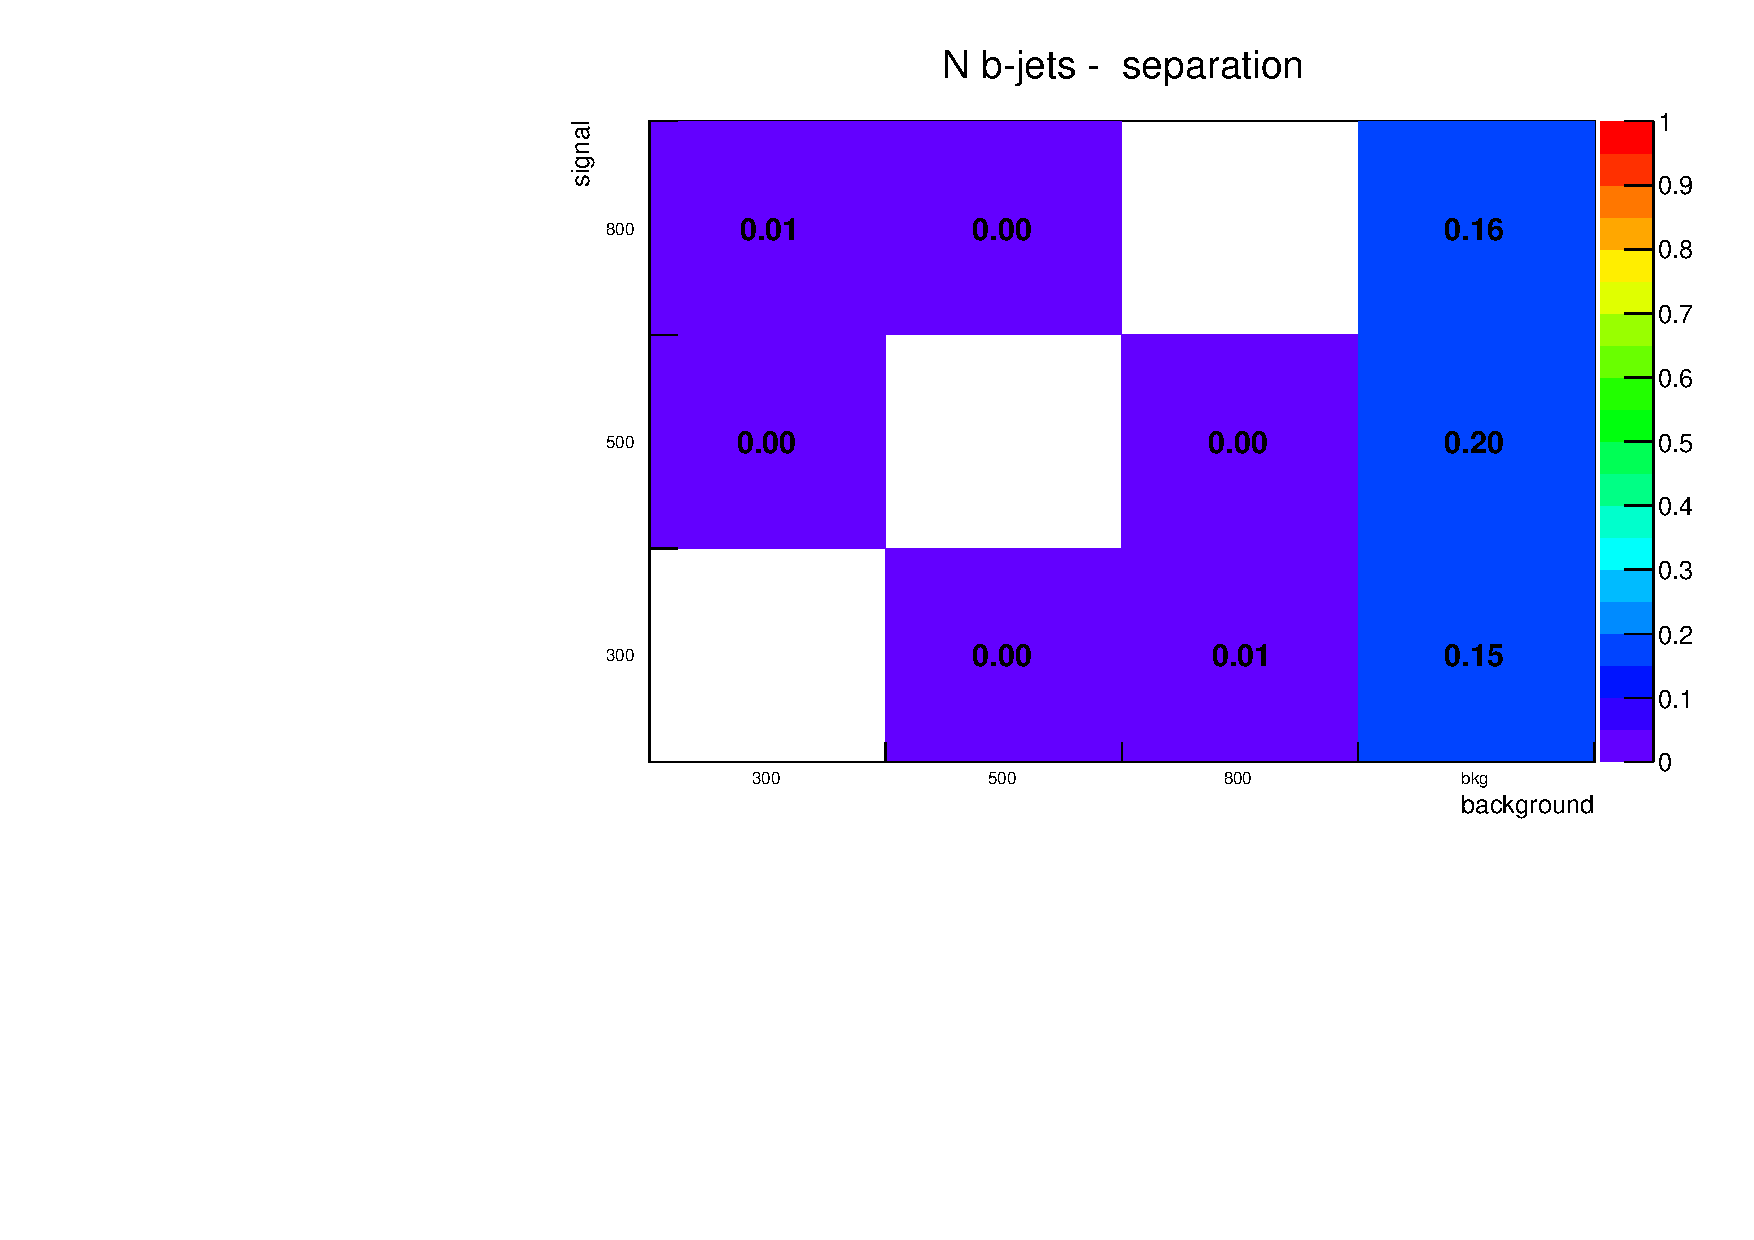
\includegraphics[width=0.43\textwidth]{figures/ewk_prod/separation/saparation_Nb_jets.pdf}}\\
\subfigure[]{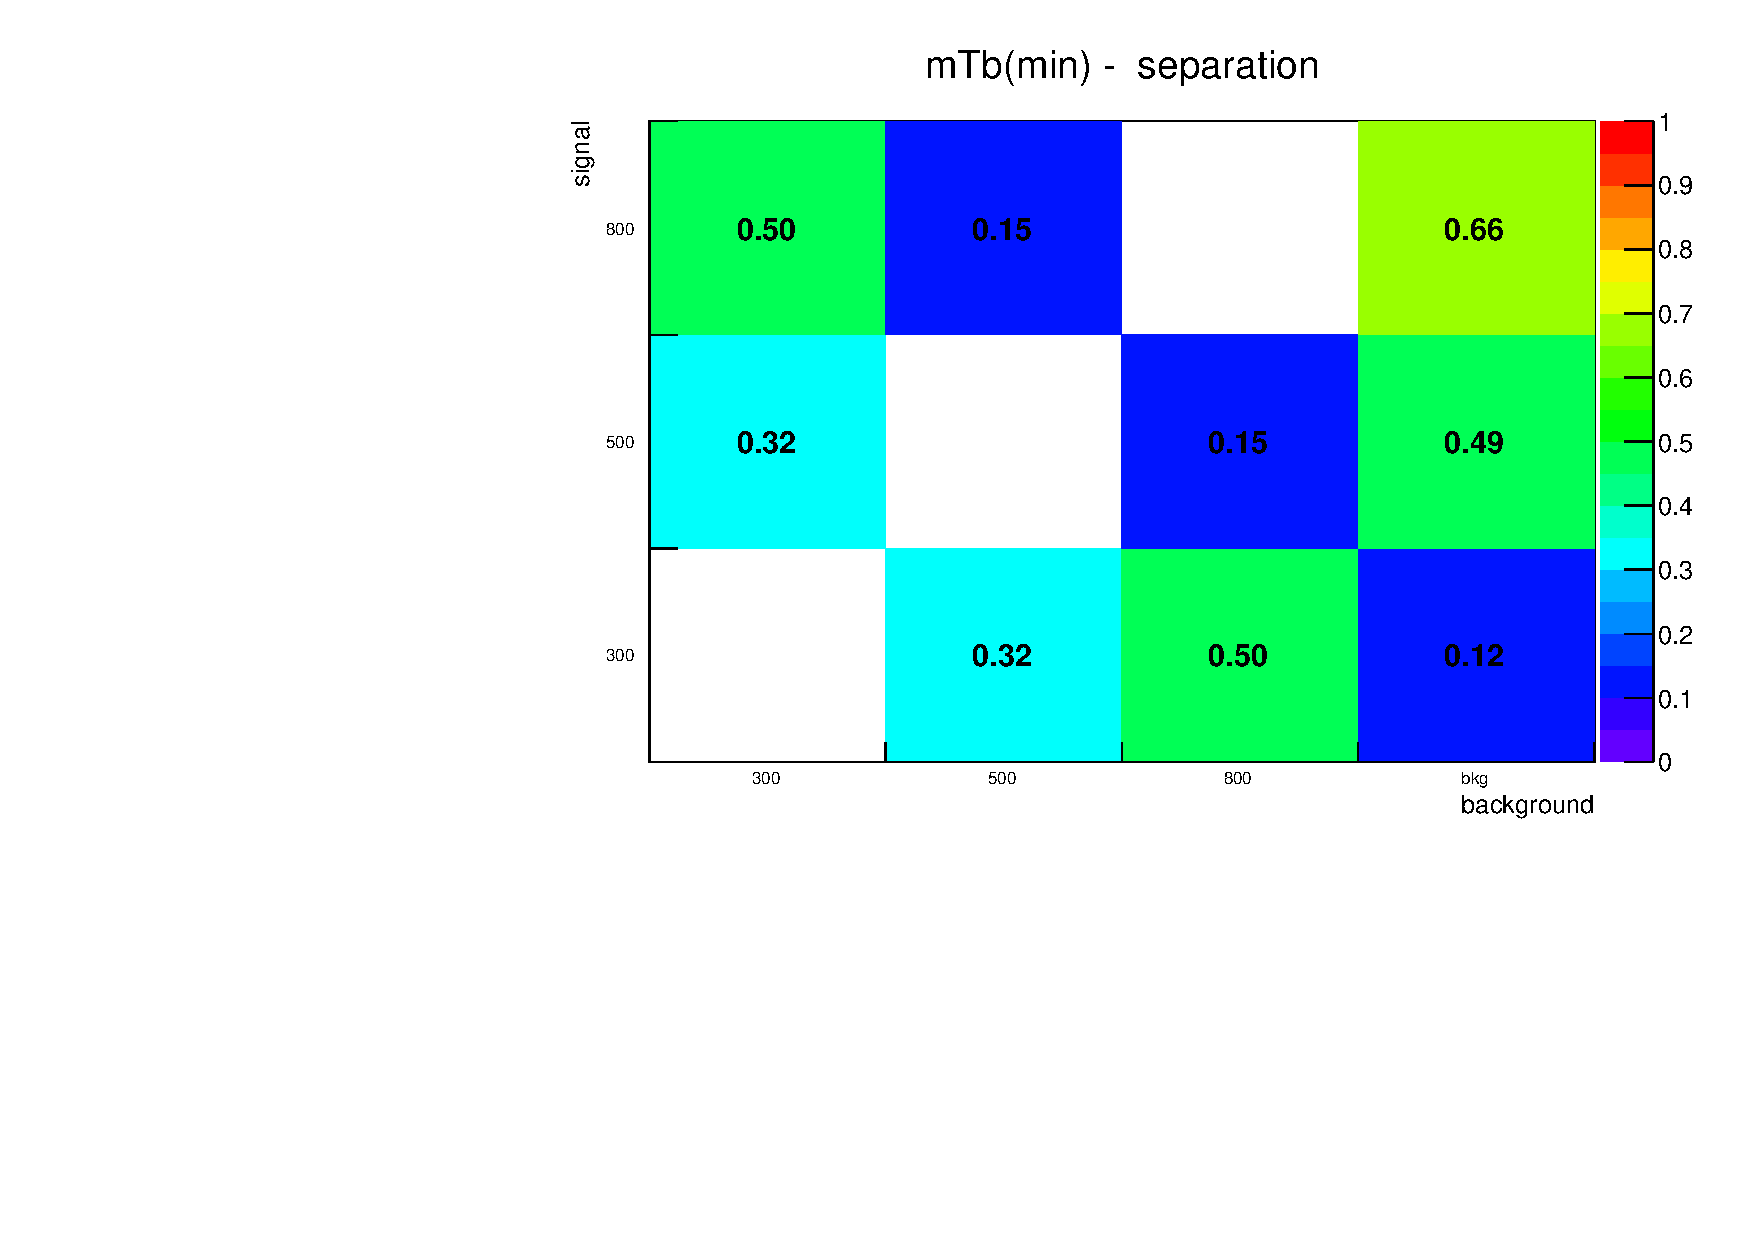
\includegraphics[width=0.43\textwidth]{figures/ewk_prod/separation/saparation_mTbmin.pdf}}
\subfigure[]{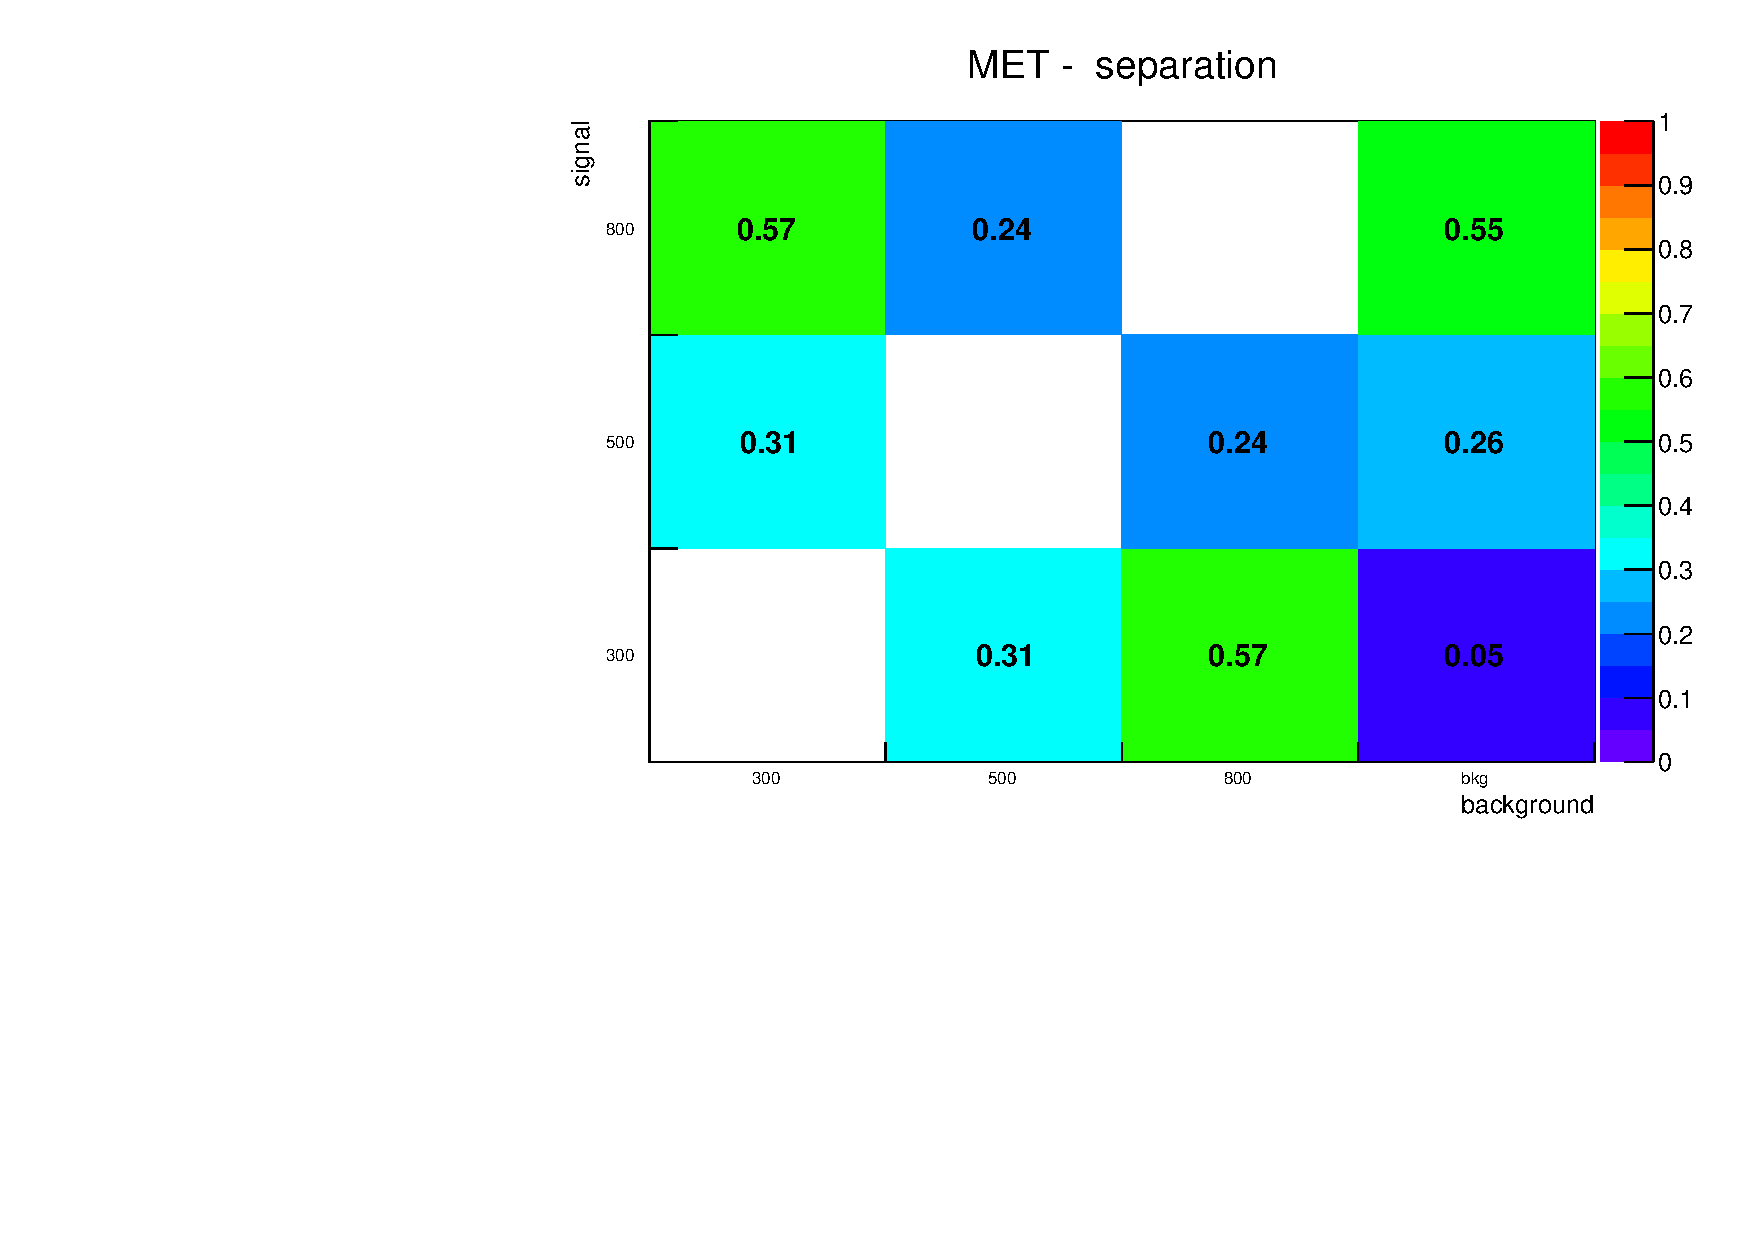
\includegraphics[width=0.43\textwidth]{figures/ewk_prod/separation/saparation_MET.pdf}}\\
%\subfigure[]{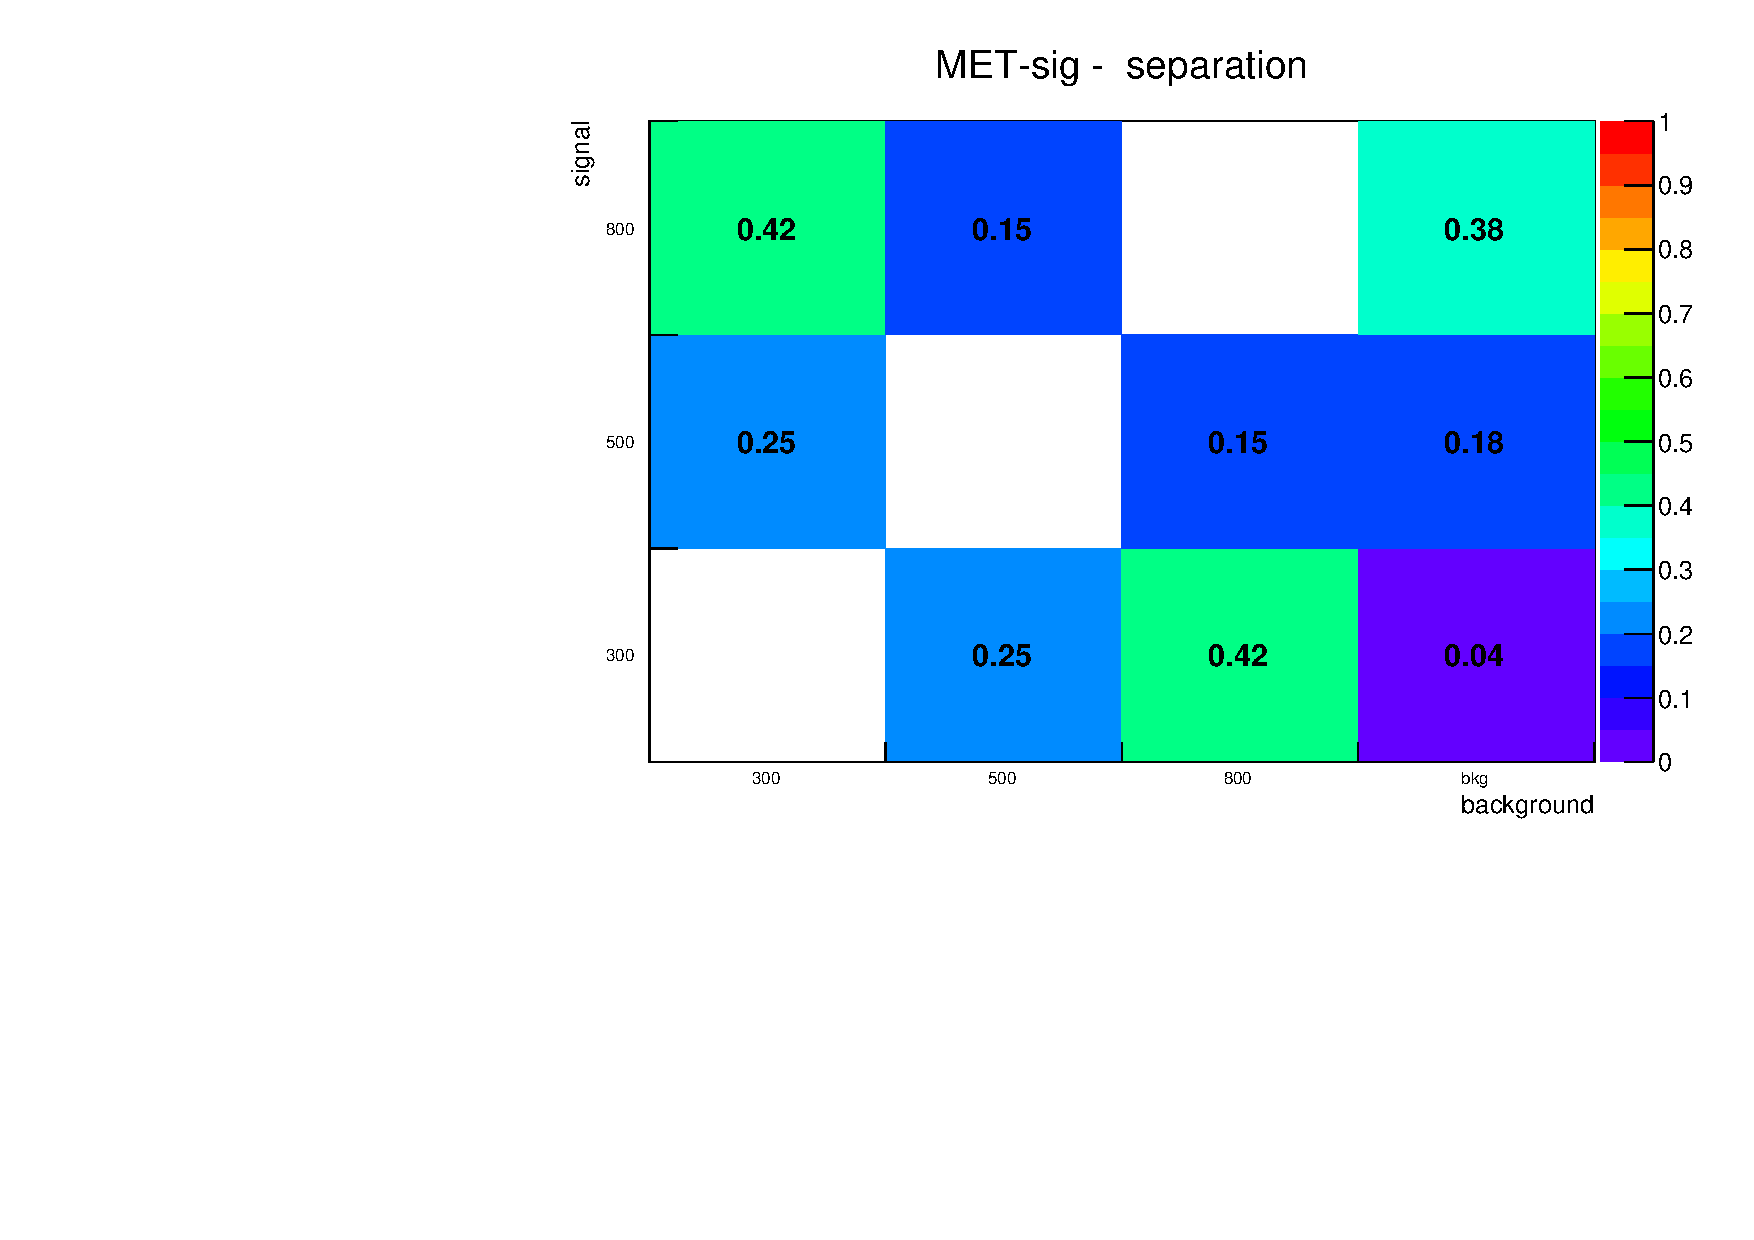
\includegraphics[width=0.43\textwidth]{figures/ewk_prod/separation/saparation_MET_sig.pdf}}
\caption{Separation offered by different analysis variables. The separation is defined as in Equation \ref{eq:separation}.}
\label{fig:ewk:separation}
\end{center}
\end{figure}

Three regular bins with a width of 150 GeV each are defined in \meffb. 
The edges of the bins are defined starting from the one with the highest value. 
At it has already been discussed in Section \ref{sec:ewk:sigbkg},
signals with high m(\hino) have kinematic features that distinguish them clearly from the background, 
but at the same time a low cross-section (e.g. for m($\ninoone$) = 800 GeV, the cross-section is about 3 fb). 
This makes it more convenient to define the selection that maximize the expected significance for a high-mass benchmark point (800 GeV) 
as a single-bin region, to concentrate as much as possible the signal events in one single \gls{sr}, 
instead of diluting it in several \glspl{sr}. % to try to exploit shape information.
The optimal selection for the high-m(\hino) benchmark signal occupies the highest \meffb bin,
and is determined my maximizing the expected significance over all the other discriminating variables,
leading to the selection:
\meffb $>$ 1100 GeV, \mtb$>$130 GeV, \dRmax $<$ 1.4, \met $>$200, $\geq$ 3 $b$-jets (77\% \gls{op}), 
4-5 jets, m($h_1$) in the range 110-150 GeV, m($h_2$) in the range 90-140 GeV.

Considering the separation power of the different variables shown in Figure  \ref{fig:ewk:separation} 
and the signal-to-background comparison in Figure \ref{fig:ewk:sig:1}, 
\dRmax is chosen as second binning variable. 
%to gain signal acceptance also for signals less boosted than the 800 GeV mass one, where the angular separation between the two $b$-jets originating from the same higgs is larger.
Once the selections for the high-\meffb \gls{sr} have been defined, 
a similar procedure is repeated for the other \meffb ranges: 600-850 GeV and 850-1100 GeV. 
These two bins with lower \meffb are also split according to the number of $b$-jets: exactly 3 and $\geq$4. 
The two bins in $b$-jet multiplicity are optimized separately. 
For each of the four remaining regions, the following steps are taken:

\begin{enumerate}
\item Optimize for one specific signal benchmark: \mhino = 300, 500 GeV for the 600-850 and 850-1100 GeV \meffb bins respectively.
\item  Where possible with a loss in significance $<$ 15\%, the selections are made uniform. 
This results to be the case for the m($h_1$) and m($h_2$) ranges, for the selection in \met, for the first bin in \dRmax, 
and for the number of jets. In the case of this last variable, it is possible to make it uniform (4-5 jets) 
without consistent loss in sensitivity in all bins except in the 4b-meff2 bin, where a veto on a 6th jet is penalizing; 
in this region, the selection on the number of jets is 4-6.
\item Use \dRmax to define further bins.
\end{enumerate}

It is found that a second bin in \dRmax is really helpful only in the regions with low and intermediate \meffb, and  $\geq$ 4 $b$-jets. 
This is because the highest \meffb region is particularly sensitive to high-mass signals, where \dRmax is small. 
For signals with lower masses, the signal-to-background ratio in regions with exactly 3 $b$-jets and high \dRmax is too low, 
while the requirement of a fourth $b$-jet suppresses the \gls{sm} background further and gives good sensitivity 
also to the region of phase space with higher \dRmax.
The final \glspl{sr} selections are summarized in Table \ref{tab:SR}.

\begin{table}[htbp]
\begin{center}
%\resizebox{1.\textwidth}{!}{
\renewcommand{\arraystretch}{1.1}
\begin{tabular}{|l|c|c|c|}
\toprule
  & SR-3b-meff1-A & SR-3b-meff2-A & SR-3b-meff3-A\\
 \hline
\nbjet &  $=$3 &  $=$3 &  $\geq$3 \\
 \hline
\met & \multicolumn{3}{|c|}{$>$ 200}\\
\hline
\dphimin    & \multicolumn{3}{|c|}{$>$0.4}\\
 \hline
\njet &  4--5 &  4--5 &  4--5 \\
 \hline
\mtb &  $>$150 &  $>$150 &  $>$130 \\
 \hline
$m(h_1)$ &    \multicolumn{3}{|c|}{110--150}\\
 \hline
$m(h_2)$ &    \multicolumn{3}{|c|}{90--140}\\
 \hline
\dRmax &  0.4--1.4 &  0.4--1.4 &  0.4--1.4 \\
 \hline
\meffb &  600--850 &  850--1100 &  $>$1100  \\
\bottomrule
\end{tabular} 

\vspace{0.4cm}

\begin{tabular}{|l|c|c|c|c|}
\toprule
   & SR-4b-meff1-A & SR-4b-meff1-B & SR-4b-meff2-A & SR-4b-meff2-B  \\
 \hline
\nbjet &  $\geq$4 &  $\geq$4 &  $\geq$4 &  $\geq$4 \\
 \hline
\met & \multicolumn{4}{|c|}{$>$ 200}\\
\hline
\dphimin    & \multicolumn{4}{|c|}{$>$0.4}\\
 \hline
\njet & 4--5 &  4--5 &  4--6 &  4--6 \\
 \hline
\mtb &   - & - & - & -  \\
 \hline
$m(h_1)$ &    \multicolumn{4}{|c|}{110--150}\\
 \hline
$m(h_2)$ &    \multicolumn{4}{|c|}{90--140}\\
 \hline
\dRmax &   0.4--1.4 &  1.4--2.4 &  0.4--1.4 &  1.4--2.4\\
 \hline
\meffb &  600--850 &  600--850 &  850--1100 &  850--1100 \\
\bottomrule
\end{tabular} 
%}
\caption{Signal region definitions for the high-mass analysis. The units of \met, \mtb, $m(h_1)$, $m(h_2)$, and \meffb are GeV. 
Table from Ref. \cite{Aaboud:2018htj}.
%These variables are defined in Section~\ref{high_event_selection}.
}
\label{tab:SR}
\end{center}
\end{table}

\subsection{Cut-and-count regions}

The analysis strategy described in Section \ref{sec:ewk:multibin} leads to a good sensitivity for exclusion across the entire mass spectrum, 
but the constraint of building orthogonal regions makes it hard to have a high discovery significance 
for signals with intermediate masses. 
To solve this problem cut-and-count \glspl{sr} are defined as well, with the goal of
providing robust regions capable of discovery of \gls{susy} signatures, 
and allowing an easier reinterpretation of the results.

The upper selection on \meffb, that makes the different \glspl{sr} orthogonal, 
is the one limiting the most the sensitivity of the individual \glspl{sr}.
In the exclusion fit this is not a problem, as the sensitivity lost in one bin is recovered in the neighbouring one. 
To define the discovery regions, all the individual \glspl{sr} are considered without the upper cut on \meffb
and the expected significance for some benchmark signal models is computed in each. 
The expected significance is computed as discussed in Section \ref{sec:example_sr}, 
assuming 36.1 \ifb of data and a flat 30\% background uncertainty. 

Figure \ref{fig:ewk:disc_sig} shows the expected significance for all the multi-bin analysis regions once the upper \meffb 
selection is removed. 
Using only the modified versions of SR-4b-meff1-A, referred to as SR-4b-meff1-A-disc, 
and SR-3b-meff3 (orange and green line respectively in the figure) allow us to have good expected sensitivity for 
all the signal considered.  
This is always $>$3 sigma for all the masses in the 300-600 GeV range, and $\approx$ 2.5 sigma for the 800 GeV signal. 
The definition of SR-4b-meff1-A-disc is reported in Table \ref{tab:SR-disc}.

\begin{figure*}[htbp]
\centering
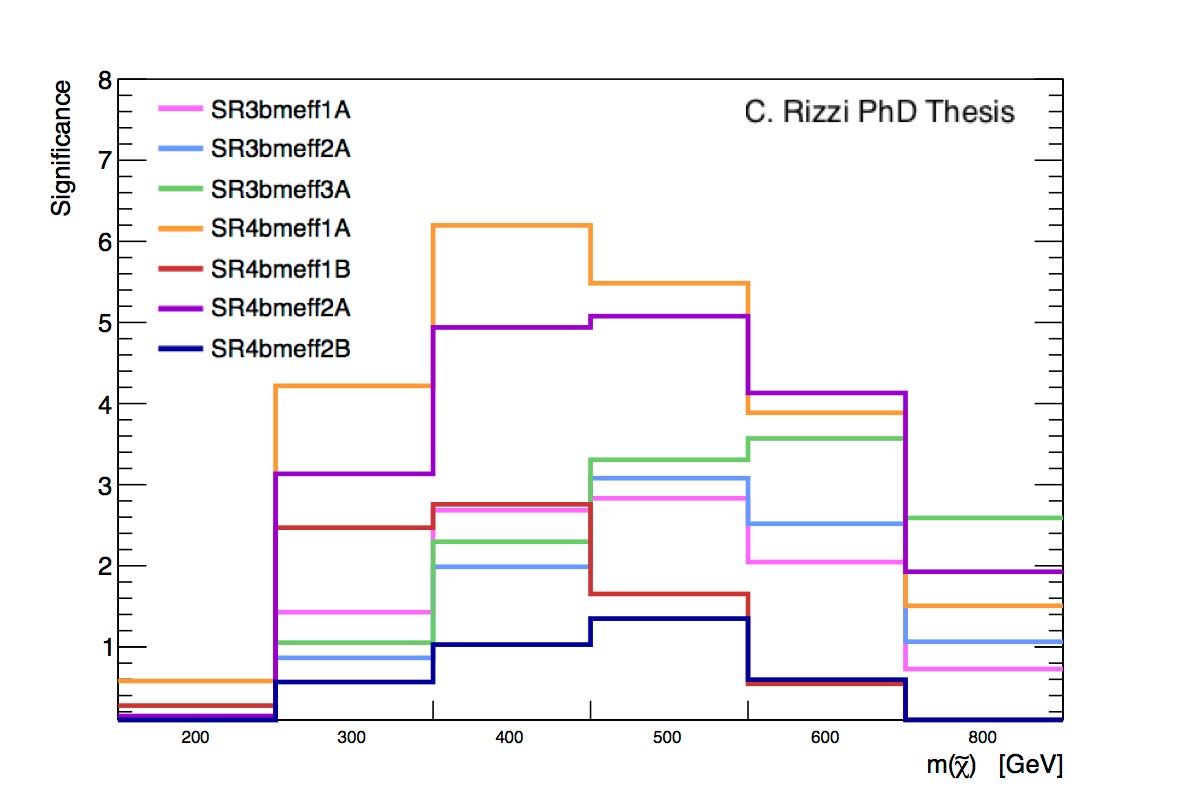
\includegraphics[width=0.7\textwidth]{figures/ewk_prod/discovery/significances_hh_regions.pdf}
\caption{Expected significance for the multi-bin regions after removing the upper \meffb selection. 
\label{fig:ewk:disc_sig}
}
\end{figure*}

\begin{table}[htbp]
\begin{center}
\renewcommand{\arraystretch}{1.1}
\begin{tabular}{|l|c|}
\toprule
   & SR-4b-meff1-A-disc \\
 \hline
\nbjet &  $\geq4$\\
 \hline
\met & $>$ 200\\
\hline
\dphimin    &$>$0.4\\
 \hline
\njet &  4--5\\
 \hline
\mtb &  - \\
 \hline
$m(h_1)$ &    110--150\\
 \hline
$m(h_2)$ &   90--140\\
 \hline
\dRmax &  0.4--1.4 \\
 \hline
\meffb &  $>600$ \\
\bottomrule
\end{tabular} 
%}
\caption{Definition of the high-mass analysis  SR-4b-meff1-A-disc. The units of \met, \mtb, $m(h_1)$, $m(h_2)$, and \meffb are GeV. 
Table from Ref. \cite{Aaboud:2018htj}.
%These variables are defined in Section~\ref{high_event_selection}.
}
\label{tab:SR-disc}
\end{center}
\end{table}


\section{Control and validation regions}

The \ttbar background is normalized in specifically designed \glspl{cr}.
A different \gls{cr} is built for each bin in \meffb and $b$-tagging multiplicity. 
These \glspl{cr} are built using side-bands both in m($h_1$) and m($h_2$). 
The extrapolation between \glspl{cr} and \glspl{sr} is tested in the \glspl{vr}, which take advantage of events
where only one between m($h_1$) and m($h_2$) is in the \gls{sr} mass range, 
as shown in Figure \ref{fig:binning_crvr}.

\begin{figure}[htbp]
	\centering
	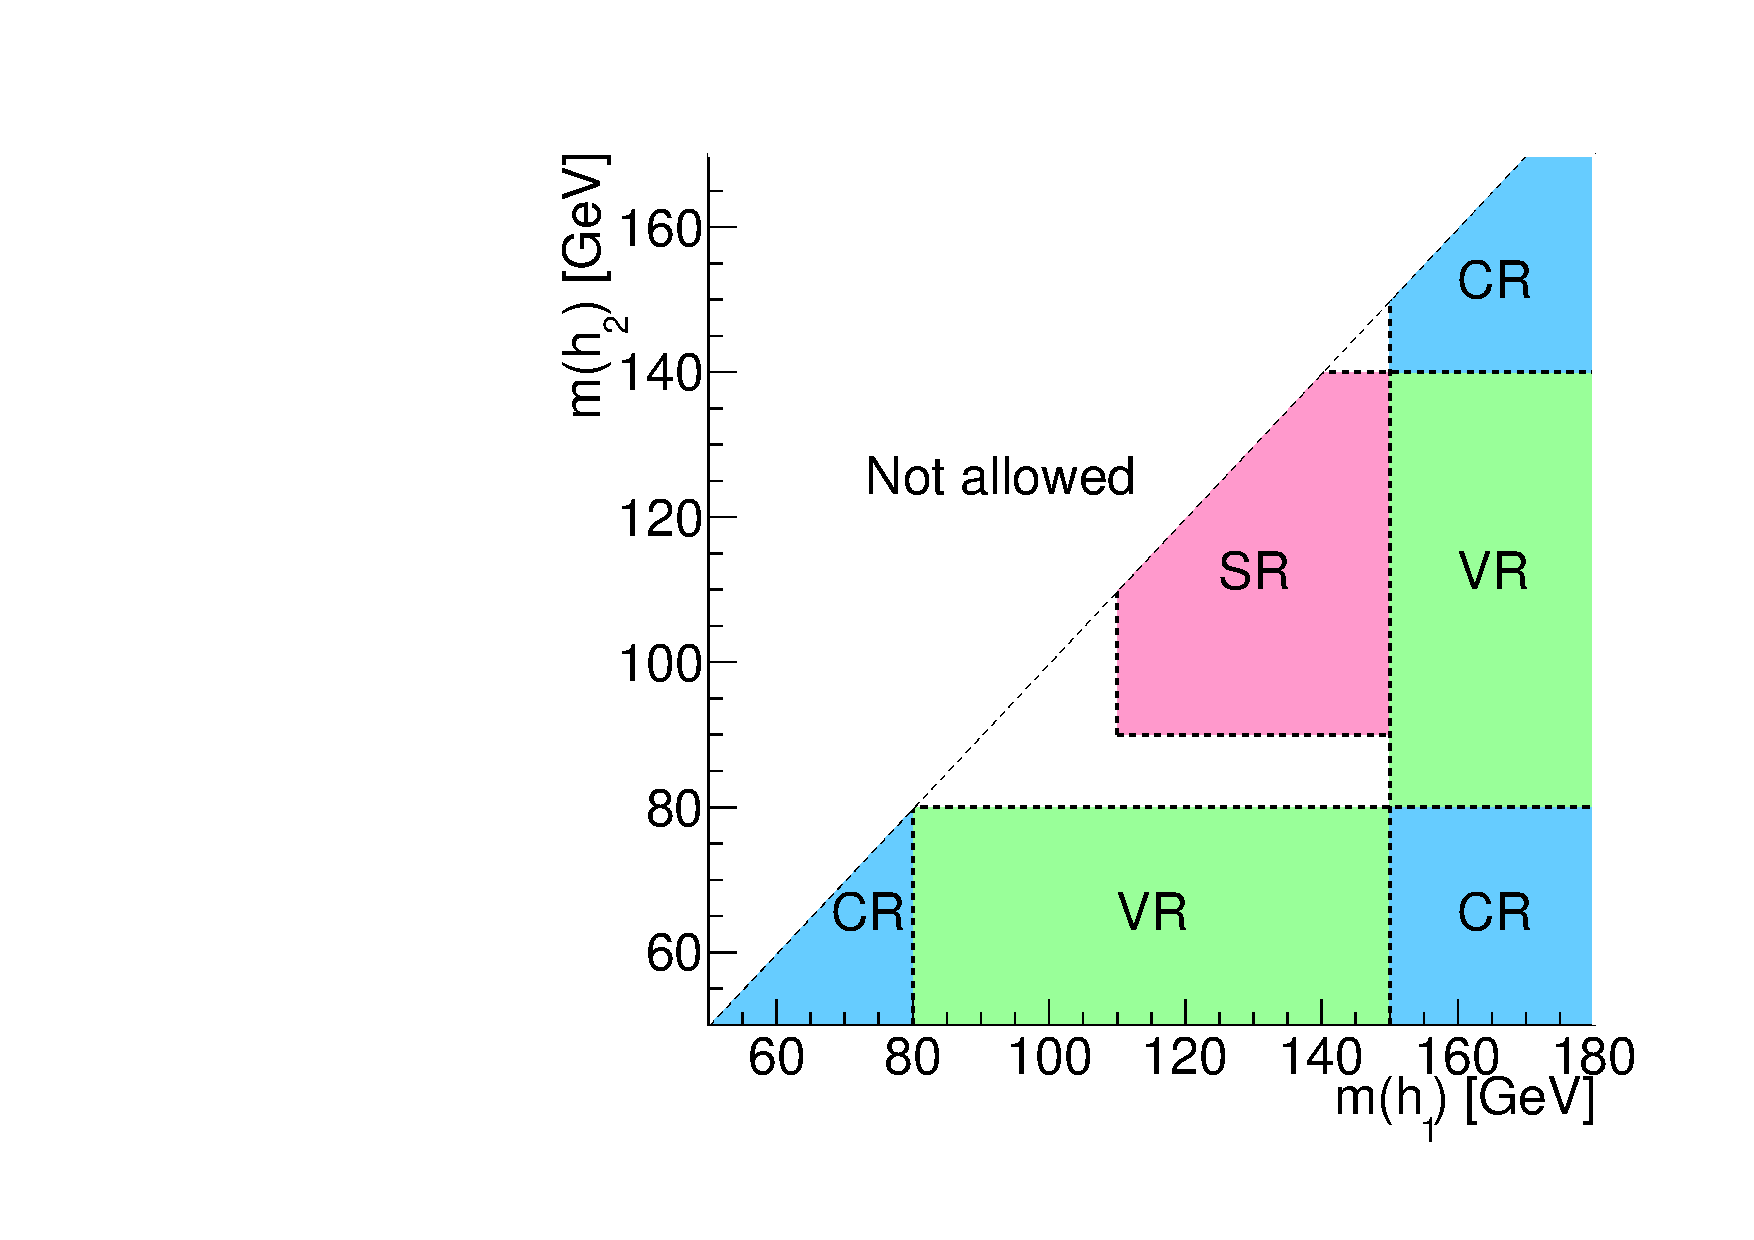
\includegraphics[width=0.490\textwidth]{figures/ewk_prod/varie/schema-1}
	\caption{The division of signal, control, and validation regions using the $m(h_1)$ and $m(h_2)$ variables in the high-mass analysis.}
	\label{fig:binning_crvr}
\end{figure}

Some of the selections of the \glspl{sr} are modified when moving to the \glspl{cr} or \glspl{vr}
 to allow enough statistics and low signal contamination.
The main extrapolation between \glspl{cr} and \glspl{sr} are:

\begin{itemize}
\item In the CR, both m($h_1$) and m($h_2$) are required to be outside the SR mass ranges.
\item \dRmax is relaxed to $<$4 (or removed).
\item \mtb is relaxed by 30 GeV in 3b-meff3 and by 50 GeV in 3b-meff1 and 3b-meff2.
\end{itemize}

To allow enough statistics in the VRs, the VRs are non orthogonal. Since these regions do not enter the fit, but are only used to validate the background prediction, non-orthogonality is not an issue here. 
The selections that remove the orthogonality between the different \glspl{vr} are:
\begin{itemize}
\item The edges of \meffb selection are relaxed by 50 GeV up and down.
\item The edges of the \dRmax bins are relaxed and, when two \dRmax bins are present for the same type of regions, they are partially overlapping.
\end{itemize}

With respect to the \glspl{sr}, the \mtb selection (where present) is relaxed as well by 50 GeV. 
Note that \glspl{cr} and \glspl{vr} do not have extrapolation in \nbjet or \njet with respect to the SRs.
The selections for all the \glspl{cr} and \glspl{vr} are summarized respectively in Tables \ref{tab:ewk:CR} and \ref{tab:ewk:VR}.


\begin{table}[htbp]
\begin{center}
%\resizebox{0.75\textwidth}{!}{
\renewcommand{\arraystretch}{1.1}
\begin{tabular}{|l|c|c|c|c|c|}
\toprule
  & CR-3b-meff1 & CR-3b-meff2 & CR-3b-meff3 & CR-4b-meff1 & CR-4b-meff2 \\
 \hline
\nbjet &  $=$3 &  $=$3 &  $\geq$3 &  $\geq$4 &  $\geq$4 \\
 \hline
\met  & \multicolumn{5}{|c|}{$>$ 200}\\
 \hline
\dphimin  & \multicolumn{5}{|c|}{$>$0.4}\\
 \hline
\njet &  4--5 &  4--5 &  4--5 &  4--5 &  4--6 \\
 \hline
\mtb &  $>$100 &  $>$100 &  $>$100 & - & - \\
 \hline
$m(h_1)$, $m(h_2)$  &  \multicolumn{5}{|c|}{ ($m(h_1)<$80, $m(h_2)<$80) or ($m(h_1)>$150, $m(h_2)<$80) or ($m(h_1)>$150, $m(h_2)>$140)    }\\
 \hline
\dRmax &  0.4--4 &  0.4--4 &  0.4--4 &  0.4--4 &  $\geq$ 0.4 \\
 \hline
\meffb &  600--850 &  850--1100 &  $>$1100 &  600--850 &  850--1100 \\
\bottomrule
\end{tabular} 
%} 
\caption{Control region definitions in the high-mass analysis. The units of \met, \mtb, $m(h_1)$, $m(h_2)$, and \meffb are GeV. 
Table from Ref. \cite{Aaboud:2018htj}.
%These variables are defined in Section~\ref{high_event_selection}.
}
\label{tab:ewk:CR}
\end{center}
\end{table}

\begin{table}[htbp]
\begin{center}
\renewcommand{\arraystretch}{1.1}
%\resizebox{1\textwidth}{!}{
\begin{tabular}{|l|c|c|c|}
\toprule
  & VR-3b-meff1-A & VR-3b-meff2-A & VR-3b-meff3-A \\
 \hline
\nbjet &  $=$3 &  $=$3 &  $\geq$3  \\
 \hline
\met  &  \multicolumn{3}{|c|}{$>$200}\\
 \hline
\dphimin &  \multicolumn{3}{|c|}{$>$0.4}\\
 \hline
\njet &  4--5 &  4--5 &  4--5 \\
 \hline
\mtb  & $>$120   & $>$100  & $>$80 \\
 \hline
$m(h_1)$, $m(h_2)$  &  \multicolumn{3}{|c|}{   (80<$m(h_1)$<150, $m(h_2)$<80) or ($m(h_1)$>150, 90<$m(h_2)$<140)   }\\
 \hline
\dRmax &  0.4--1.5 &  0.4--1.7 &  0.4--1.7  \\
 \hline
\meffb   & 550--900   & 800--1150  & $>$1050    \\
\bottomrule
\end{tabular} 

\vspace{0.4cm}

\begin{tabular}{|l|c|c|c|c|}
\toprule
  &  VR-4b-meff1-A & VR-4b-meff1-B & VR-4b-meff2-A & VR-4b-meff2-B \\
 \hline
\nbjet &   $\geq$4 &  $\geq$4 &  $\geq$4 &  $\geq$4 \\
 \hline
\met  &  \multicolumn{4}{|c|}{$>$200}\\
 \hline
\dphimin &  \multicolumn{4}{|c|}{$>$0.4}\\
 \hline
\njet &   4--5 &  4--5 &  4--6 &  4--6 \\
 \hline
\mtb   &  \multicolumn{4}{|c|}{-}\\
 \hline
$m(h_1)$, $m(h_2)$  &  \multicolumn{4}{|c|}{   (80<$m(h_1)$<150, $m(h_2)$<80) or ($m(h_1)$>150, 90<$m(h_2)$<140)   }\\
 \hline
\dRmax &   0.4--1.7 &  1.4--3 &  0.4--1.7 &  1.4--3 \\
 \hline
\meffb   &  550--900  & 550--900  & 800--1150  & 800--1150  \\
\bottomrule
\end{tabular} 
%} 
\caption{Validation region definitions in the high-mass analysis. The units of \met, \mtb, $m(h_1)$, $m(h_2)$, and \meffb are GeV. 
Table from Ref. \cite{Aaboud:2018htj}.
%These variables are defined in Section~\ref{high_event_selection}.
}
\label{tab:ewk:VR}
\end{center}
\end{table}

\section{Background composition}

The pre-fit background composition of the analysis regions is show in Figures \ref{fig:bkgcomp_hh3b} and \ref{fig:bkgcomp_hh4b}.
It is possible to see how \ttbar is the dominant background in all the \glspl{sr}.
%The \glspl{cr} and the \glspl{vr} have a high \ttbar purity by construction. 
%, since they are designed to respectively normalize this background and validate the extrapolation of this normalization to 
%a phase space closer to the \glspl{sr}.
% chiara: change, sentence from paper
The subdominant background contributions are $Z(\to \nu\nu)$+jets and $W(\to \ell\nu)$+jets events.
%where for W+jets events the lepton is electron or muon that is not reconstructed or a hadronically decaying $\tau$-lepton. 
%In the 1-lepton \glspl{sr}, the subdominant backgrounds are single-top, \ttbar+W and \ttbar+Z.
Figures \ref{fig:ttcomp_hh3b} and \ref{fig:ttcomp_hh3b} show the decay type of the \ttbar background,
while the heavy-flavor composition of the jets that are produced together with the \ttbar pair is shown 
in Figures \ref{fig:HFcomp_hh3b} and \ref{fig:HFcomp_hh3b}.

\begin{figure}[htbp]
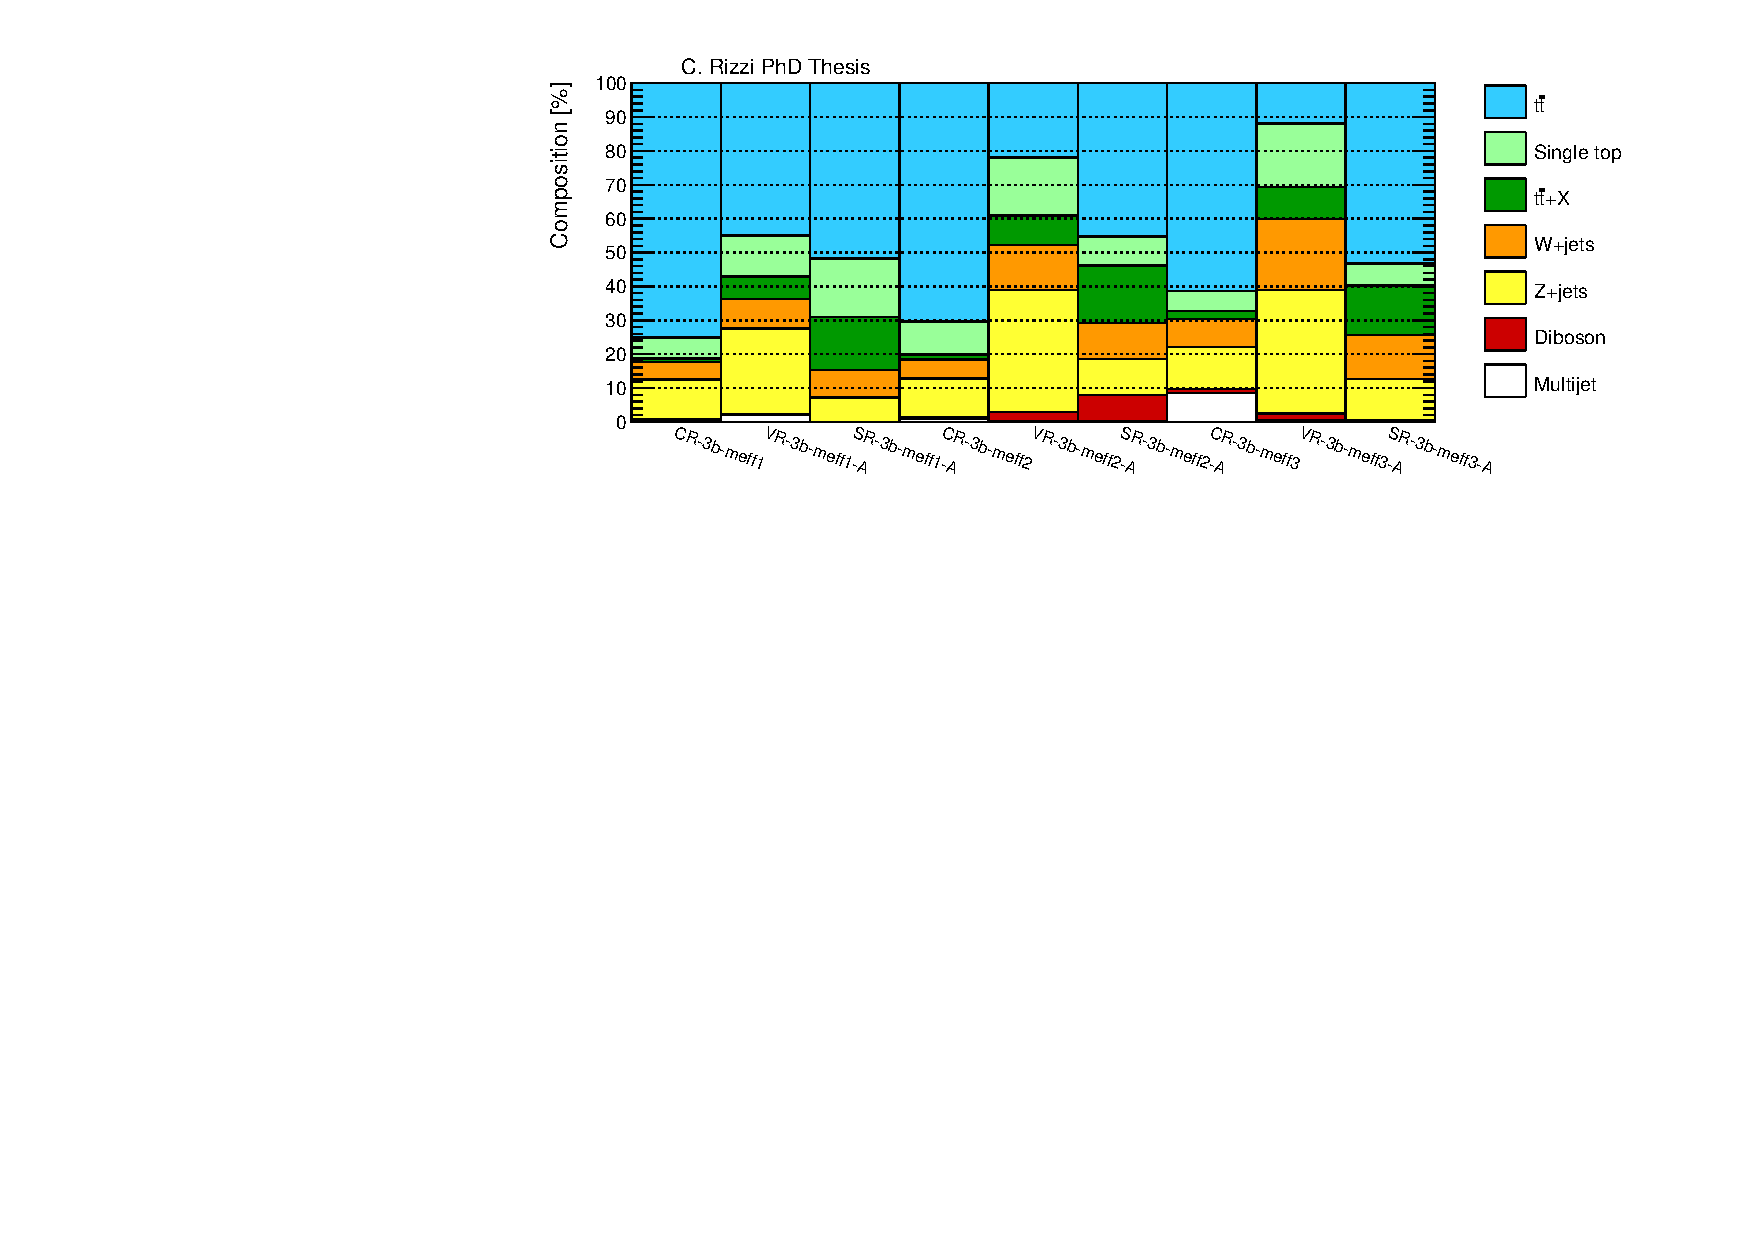
\includegraphics[width=\textwidth]{figures/ewk_prod/comp_plots/hh_3b_bkg.pdf}
\caption{Background composition in the regions with exactly three $b$-jets.}
	\label{fig:bkgcomp_hh3b}
\end{figure}

\begin{figure}[htbp]
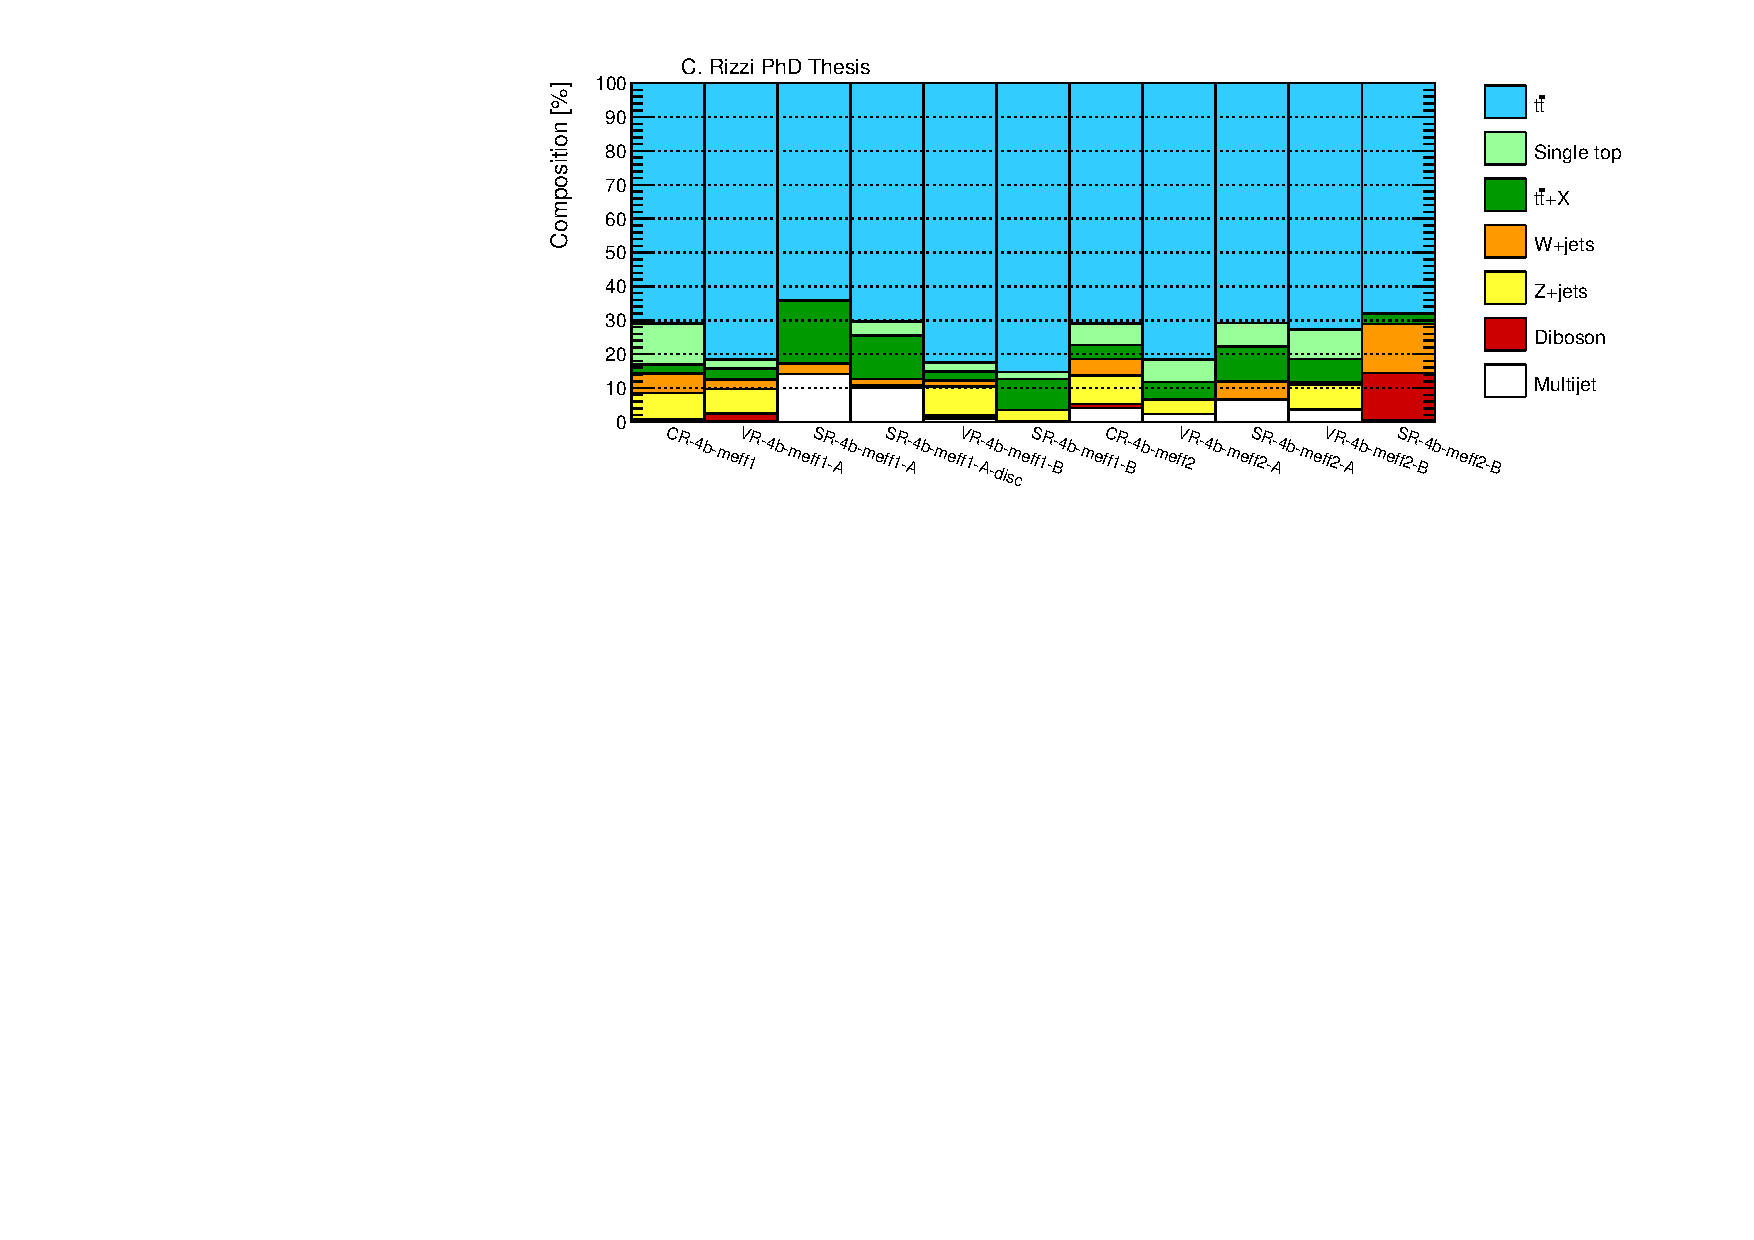
\includegraphics[width=\textwidth]{figures/ewk_prod/comp_plots/hh_4b_bkg.pdf}
\caption{Background composition in the regions with at least four $b$-jets.}
	\label{fig:bkgcomp_hh4b}
\end{figure}

\begin{figure}[htbp]
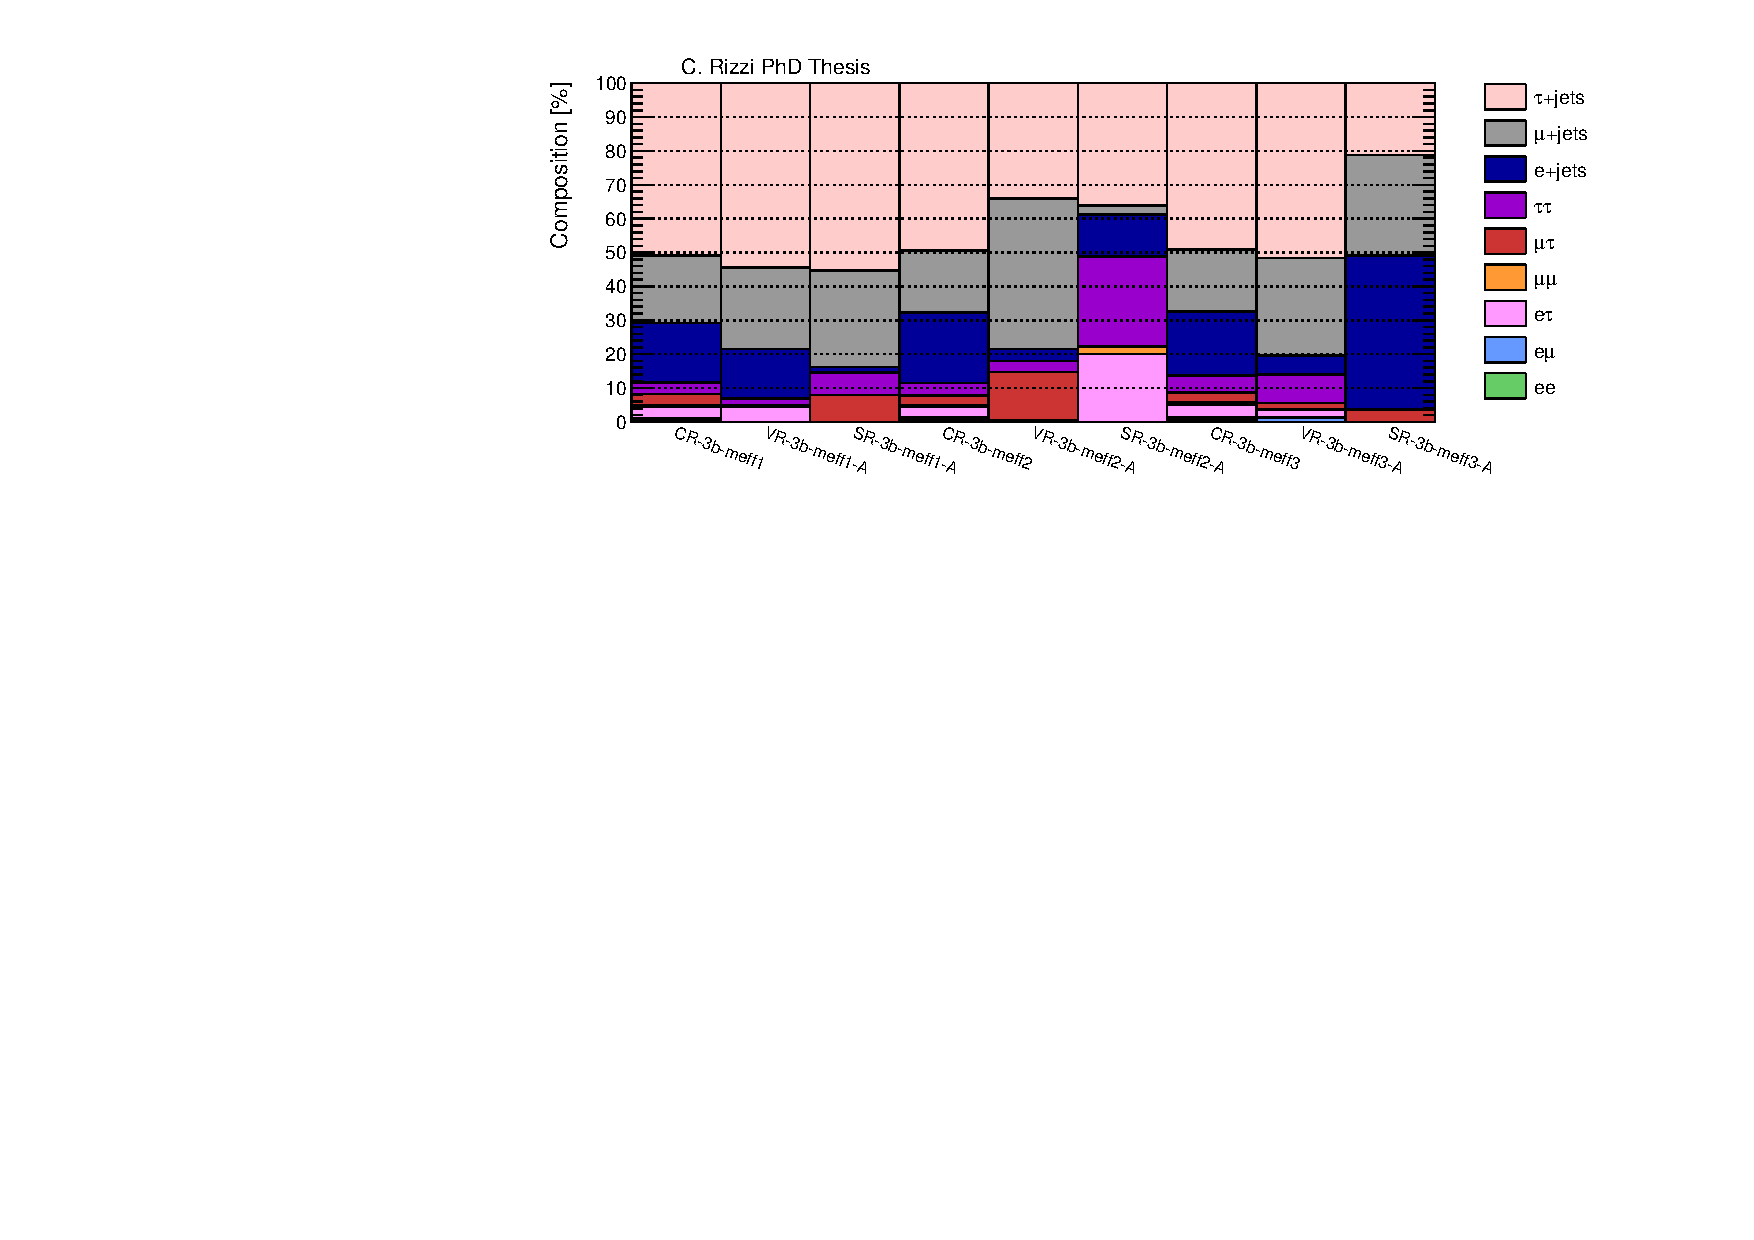
\includegraphics[width=\textwidth]{figures/ewk_prod/comp_plots/hh_3b_tt.pdf}
\caption{Decay mode of the \ttbar background in the regions with exactly three $b$-jets.}
	\label{fig:ttcomp_hh3b}
\end{figure}

\begin{figure}[htbp]
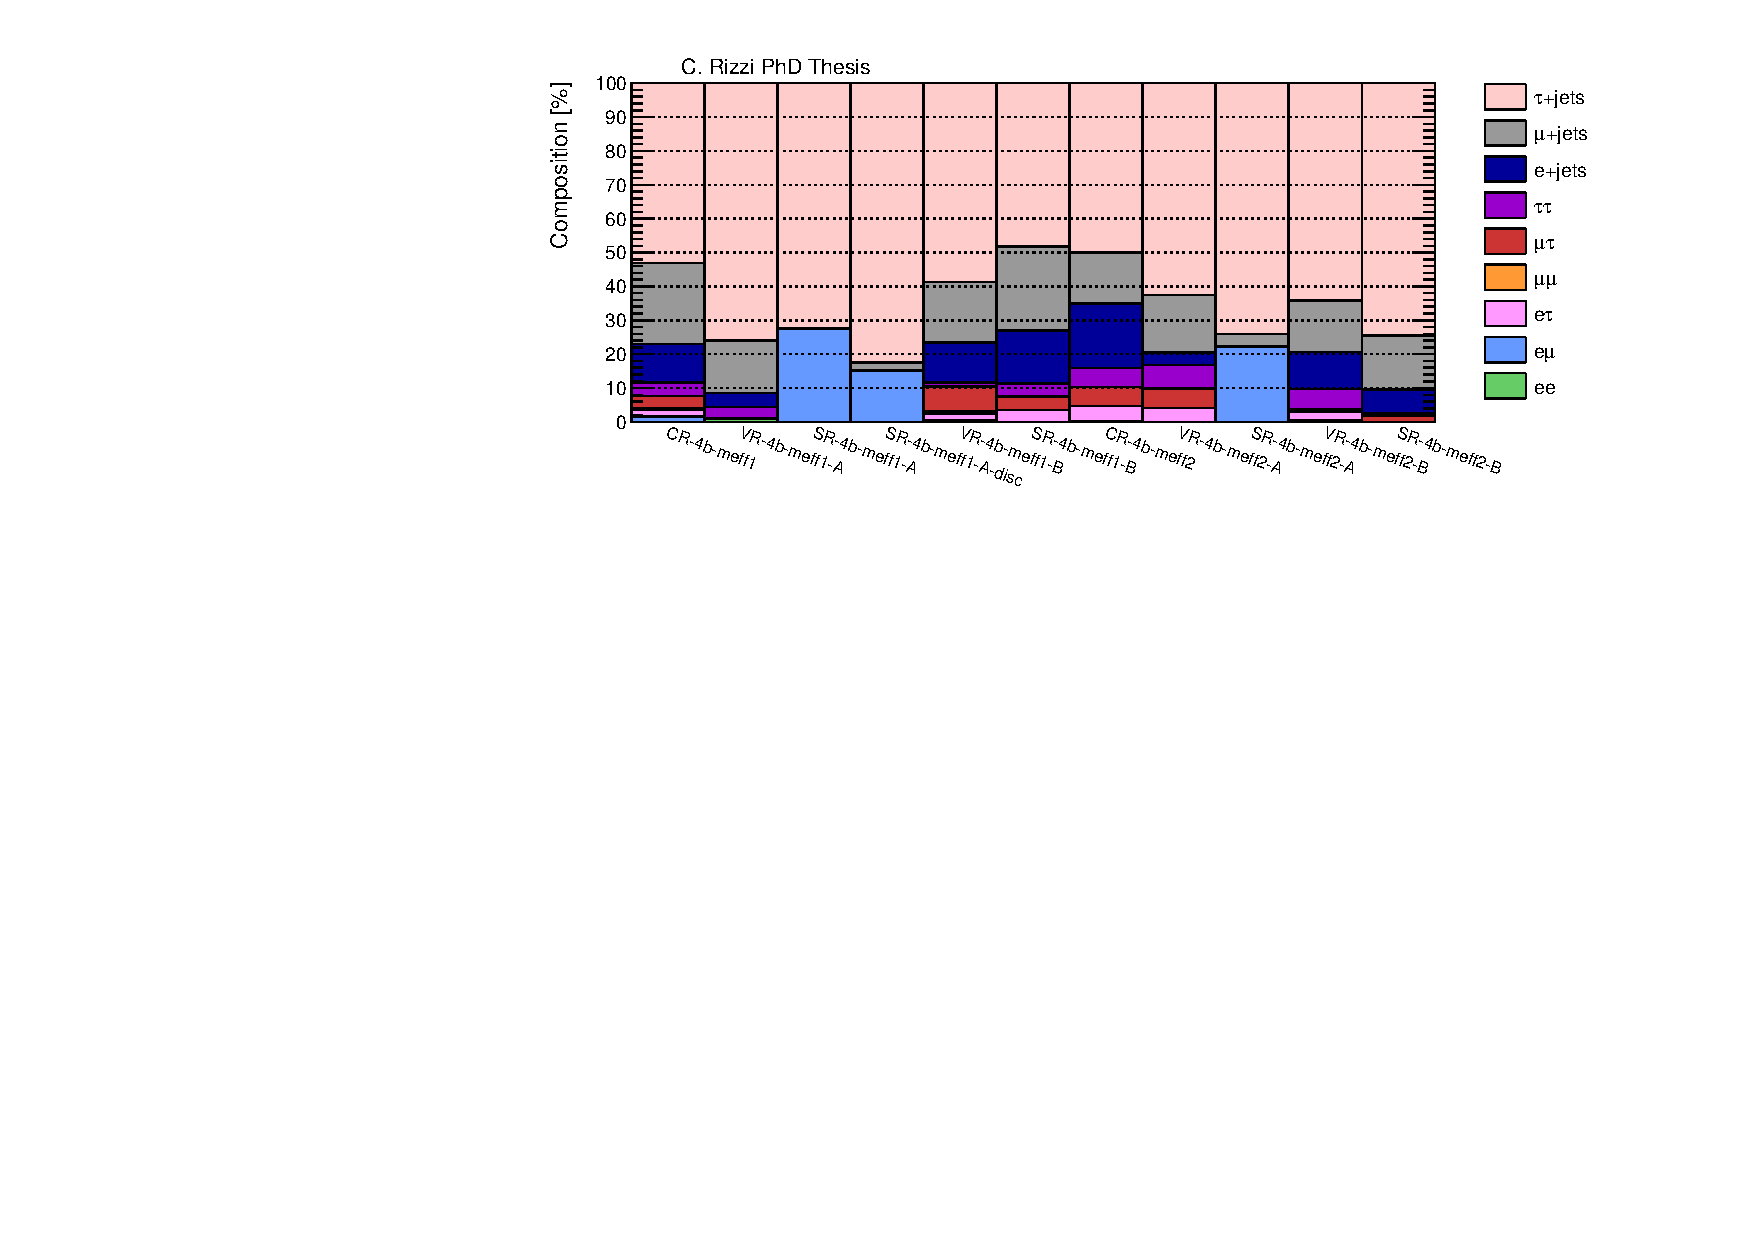
\includegraphics[width=\textwidth]{figures/ewk_prod/comp_plots/hh_4b_tt.pdf}
\caption{Decay mode of the \ttbar background in the regions with at least four $b$-jets.}
	\label{fig:ttcomp_hh4b}
\end{figure}

\begin{figure}[htbp]
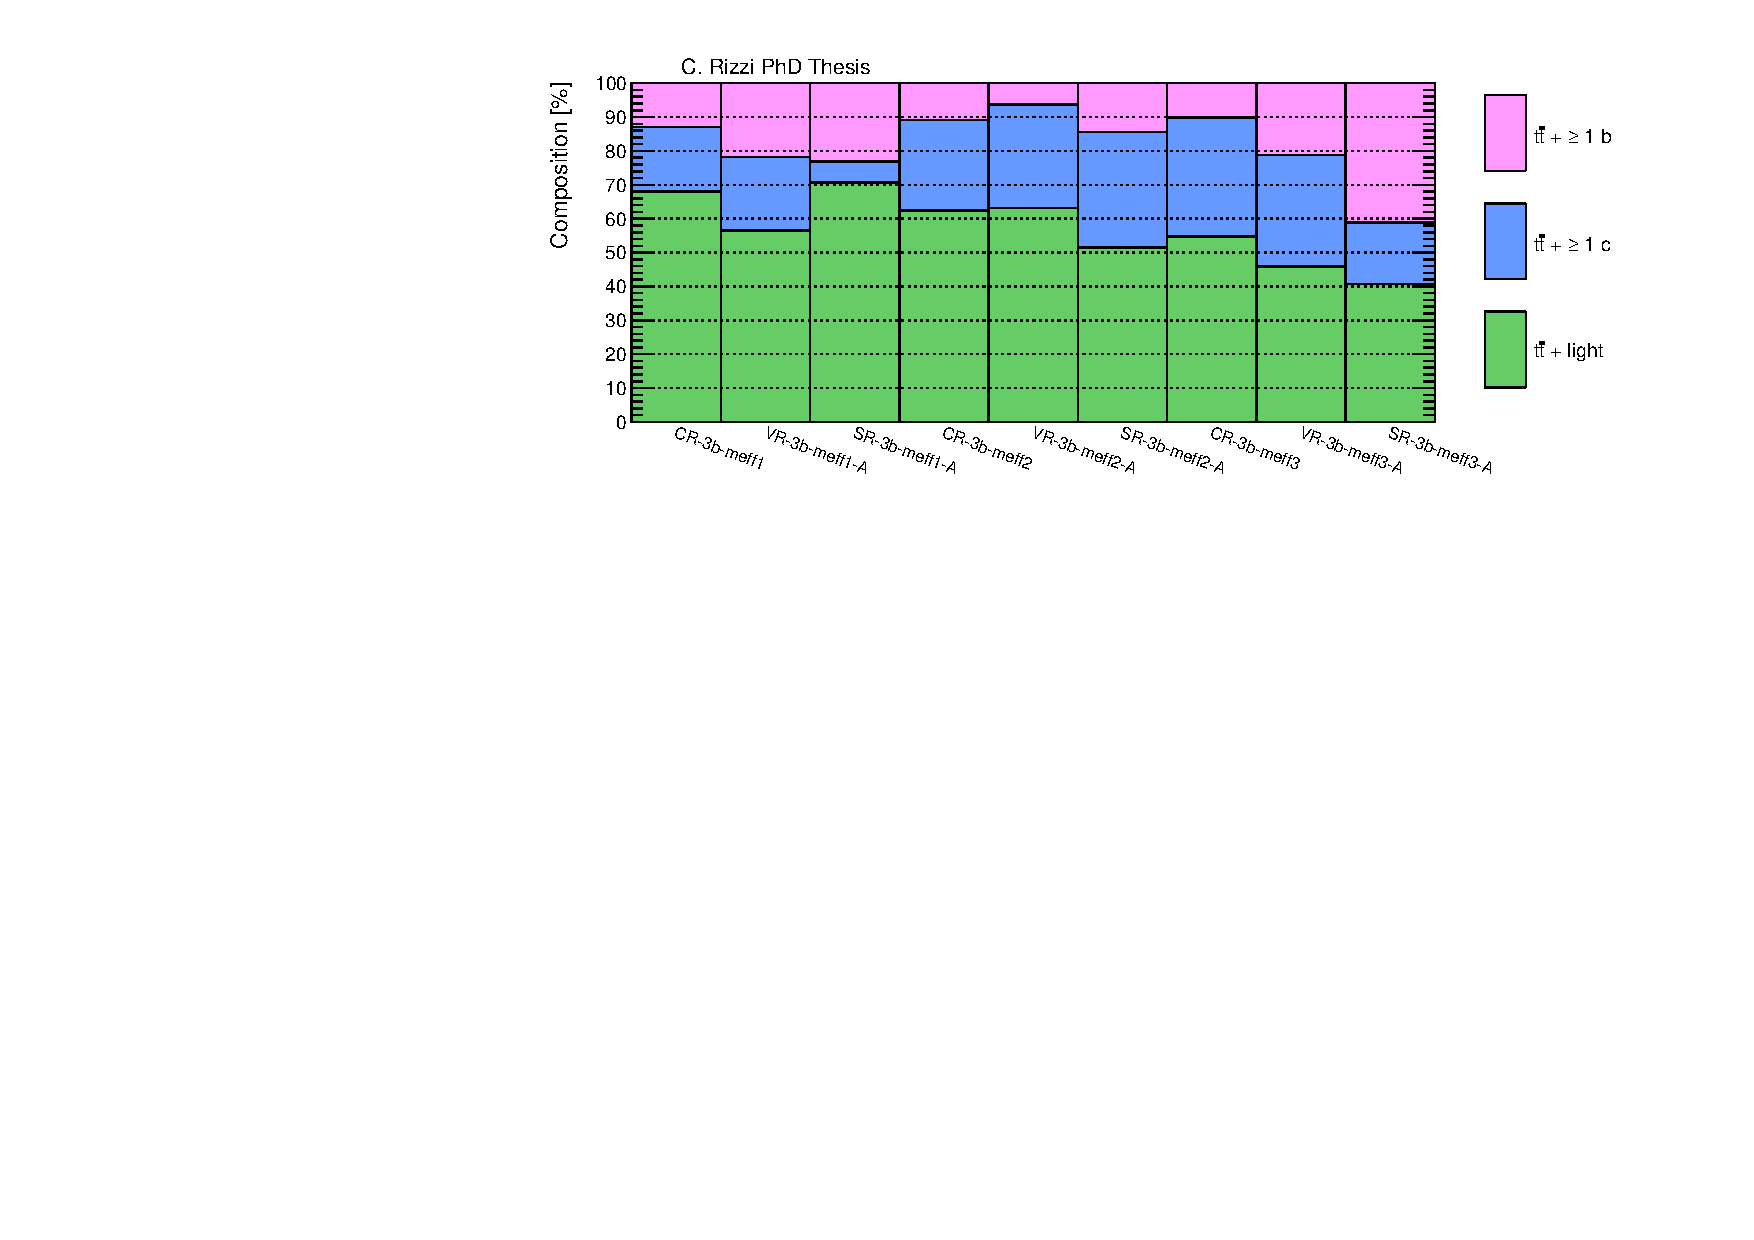
\includegraphics[width=\textwidth]{figures/ewk_prod/comp_plots/hh_3b_HF.pdf}
\caption{Heavy-flavor composition of the \ttbar background in regions with exactly three $b$-jets.}
	\label{fig:HFcomp_hh3b}
\end{figure}

\begin{figure}[htbp]
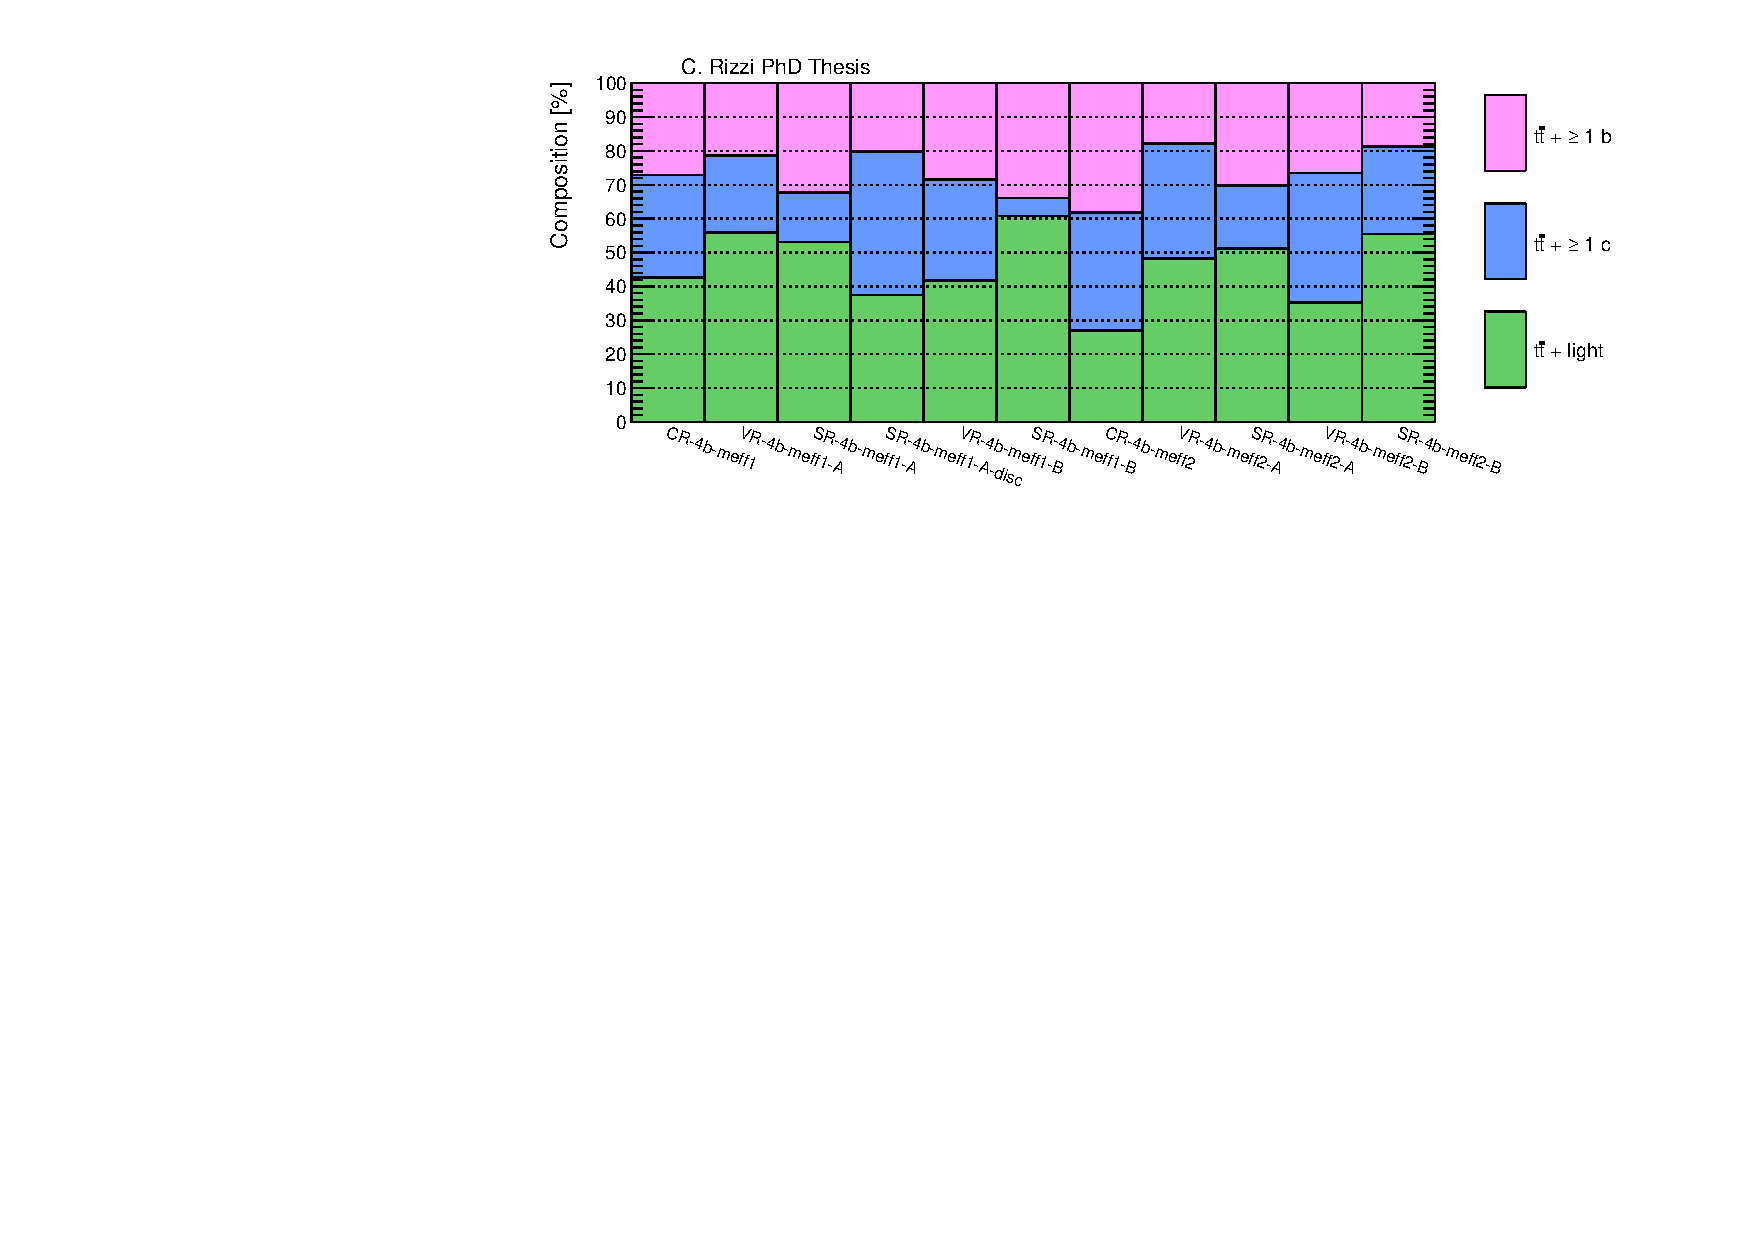
\includegraphics[width=\textwidth]{figures/ewk_prod/comp_plots/hh_4b_HF.pdf}
\caption{Heavy-flavor composition of the \ttbar background in regions with at least four $b$-jets.}
	\label{fig:HFcomp_hh4b}
\end{figure}

\FloatBarrier

\section{Comparison between data and MC}

The modelling of the main kinematic variables is very similar to what observed in Section \ref{sec:strong:dataMC} 
for the strong-production multi-b analysis, as the few differences in object definitions are not enough to 
lead to a substantial change in the agreement between data and simulation; 
this section therefore focuses on the variables specific to Higgs boson reconstruction.
The comparison between data and simulation for the variables already shown in Section \ref{sec:strong:dataMC} but with the object definitions 
specific to this analysis are shown in Appendix \ref{app:ewk:datamc}.
There is nevertheless a notable exception: in the analysis described in this chapter, the agreement between data and simulation in the 
distribution of the number of $b$-jets is improved, as can be appreciated comparing Figure \ref{fig:strong:datamc0L:bjets_n} with Figure \ref{fig:ewk:datamc_bjets}.
This is the result of the improvement in the $b$-tagging calibration: as discussed in Section \ref{sec:obj:btaggingcalib}, 
the calibration of $c$-jets used in this analysis is based on \ttbar events, rather than on $W+c$ events as in the gluino analysis.
The other important difference with respect to the strong-production analysis is that in this case the analysis is performed 
only in regions with a lepton veto; it is not therefore sensitive to the mismodelling in the 1-lepton channel discussed in Section 
\ref{sec:strong:kinrw} and no kinematic reweighting is required. 

As shown in Figure \ref{fig:ewk:datamc_a}, all the variables specific to this analysis show a good 
agreement between data and the \gls{mc} simulation. 

\begin{figure*}[htbp]
\centering 
%\subfigure[\nbjet]{
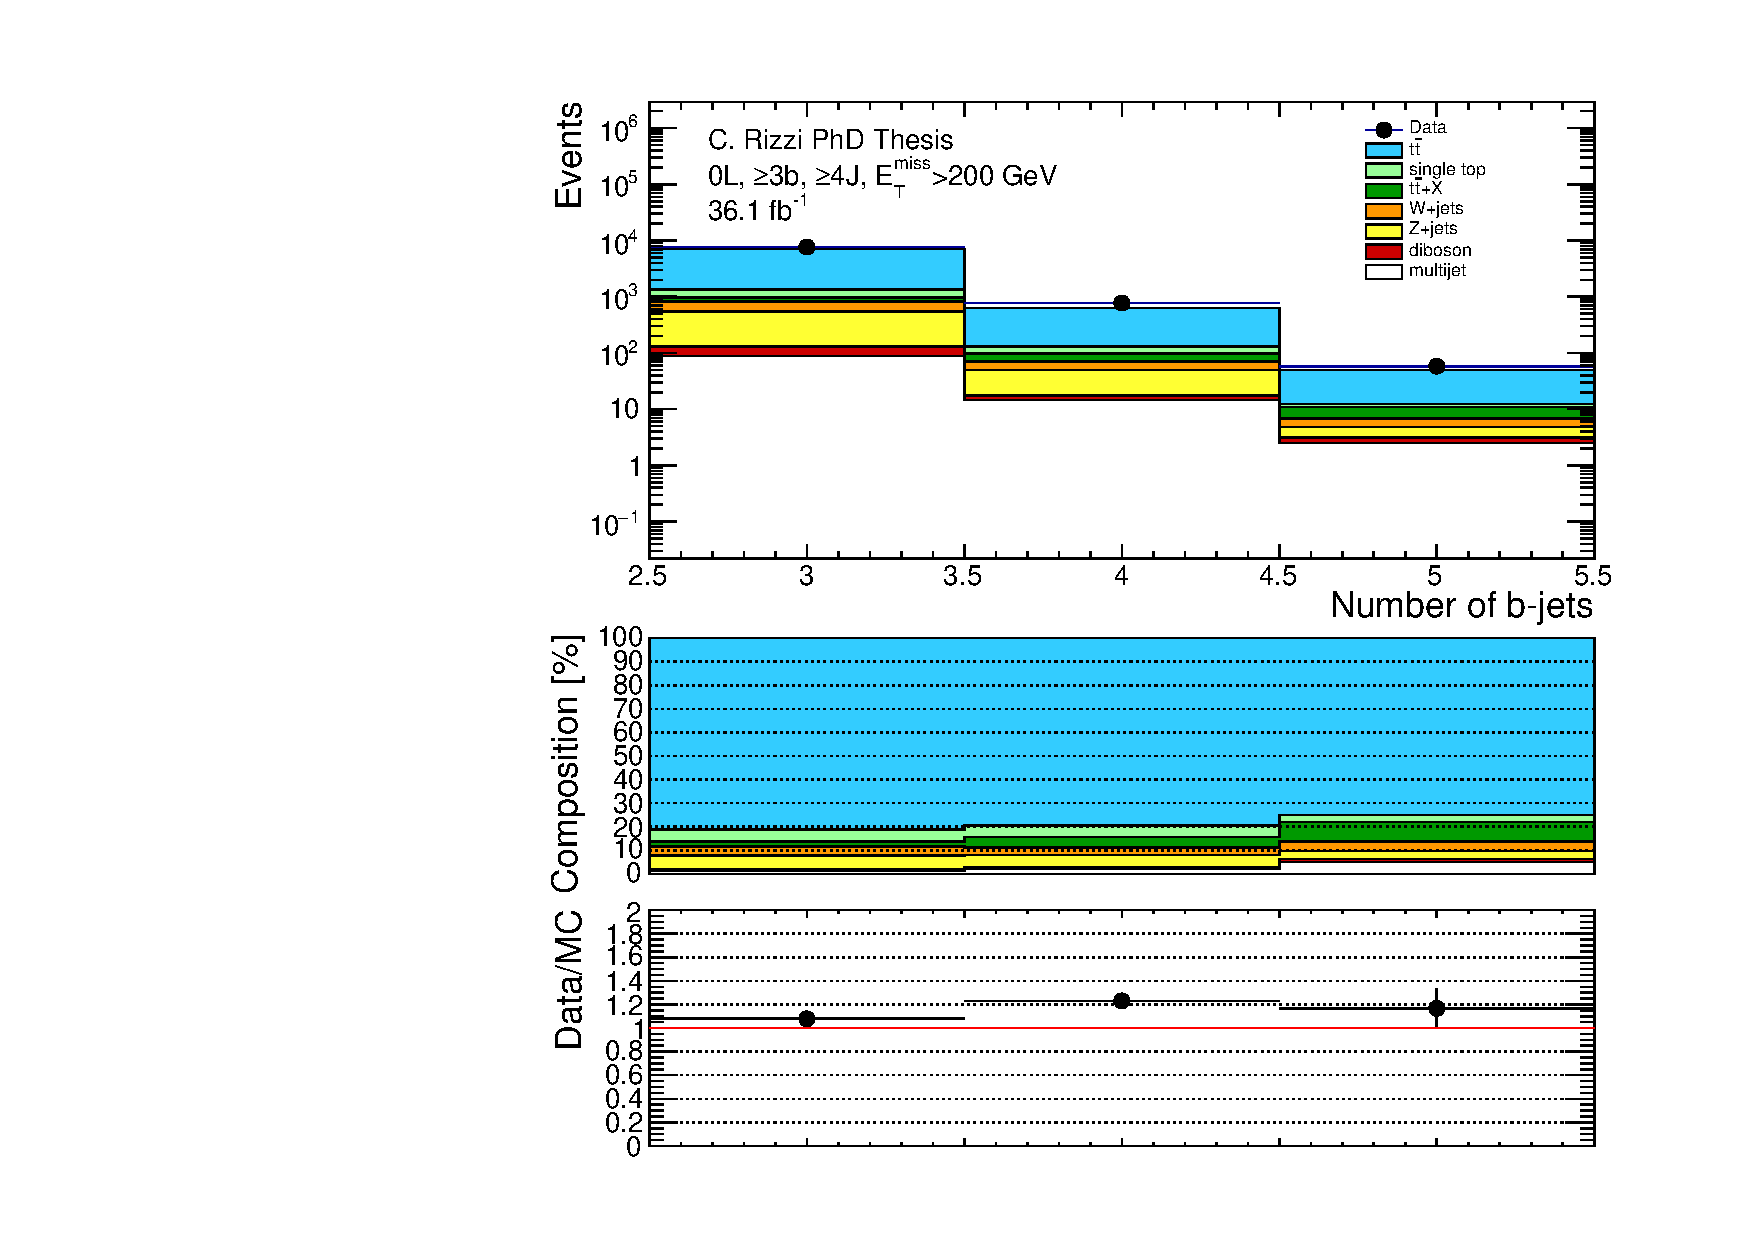
\includegraphics[width=0.45\textwidth]{figures/ewk_prod/data_mc/0L_3bin/data_mc_bjets_n.pdf}
%\label{fig:ewk:datamc:bjets_n}}\\
\caption{Comparison of the number of $b$-jets between data and simulation in the preselection described in the text.
}
\label{fig:ewk:datamc_bjets}
\end{figure*}

\begin{figure*}[htbp]
\centering 
\subfigure[m($h_1$)]{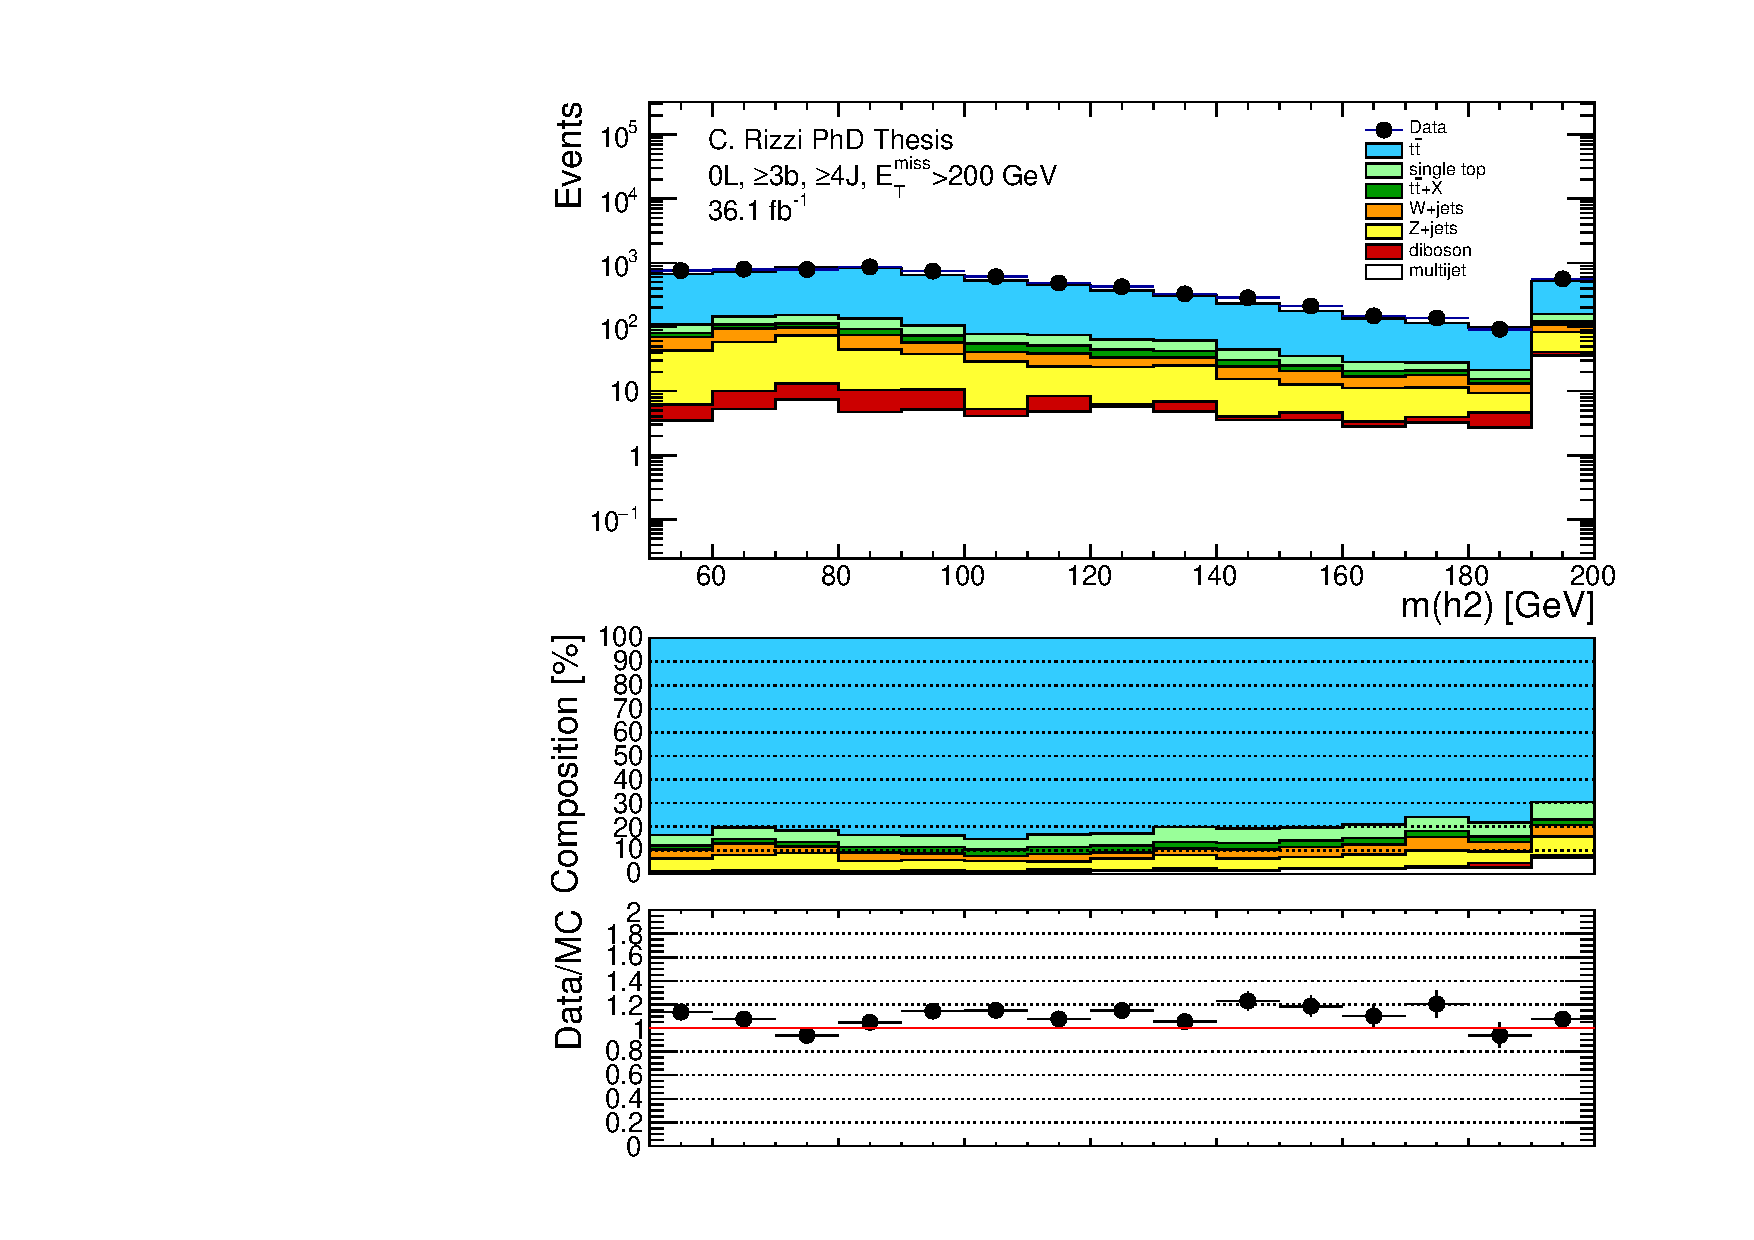
\includegraphics[width=0.45\textwidth]{figures/ewk_prod/data_mc/0L_3bin/data_mc_mass_h2_min_dR.pdf}
\label{fig:ewk:datamc:mass_h2_min_dR}}
\subfigure[m($h_2$)]{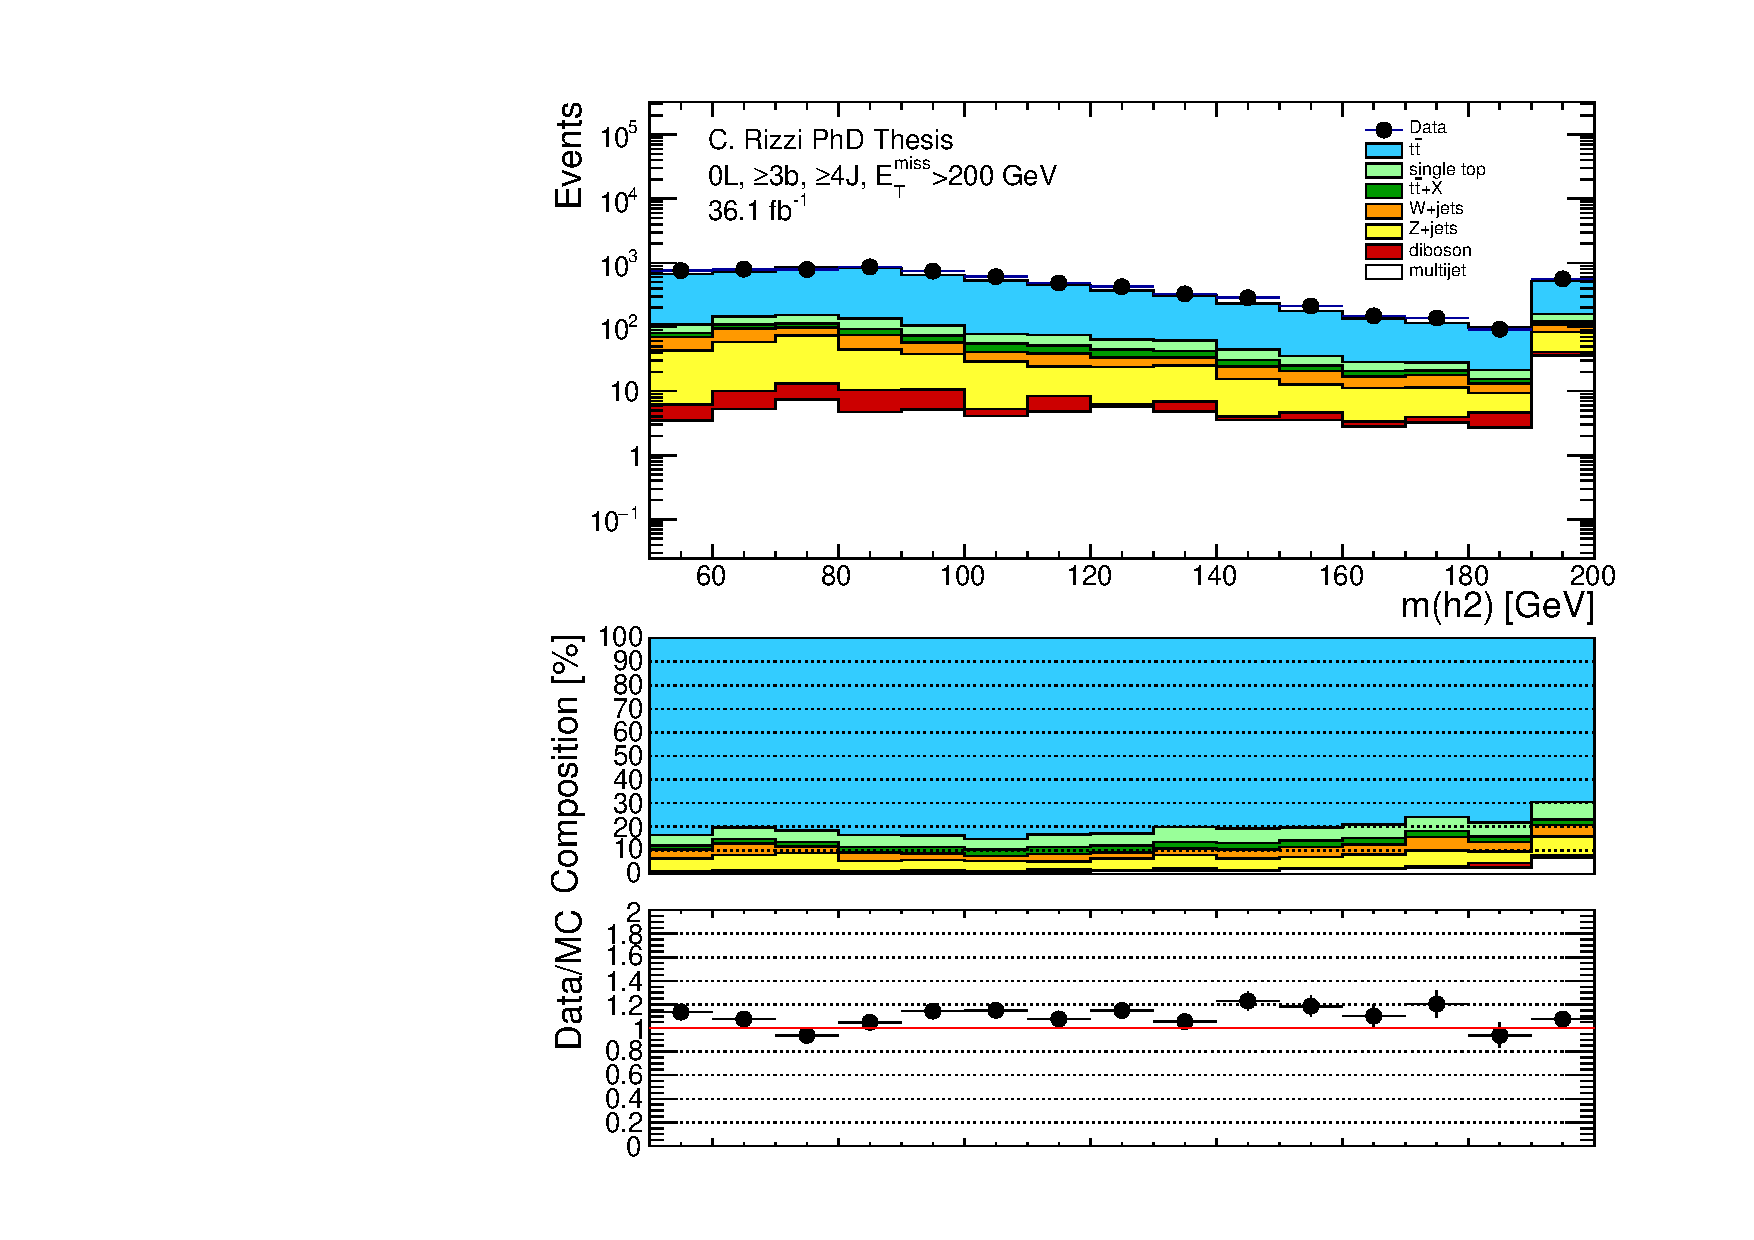
\includegraphics[width=0.45\textwidth]{figures/ewk_prod/data_mc/0L_3bin/data_mc_mass_h2_min_dR.pdf}
\label{fig:ewk:datamc:mass_h2_min_dR}}\\
\subfigure[\dRmax]{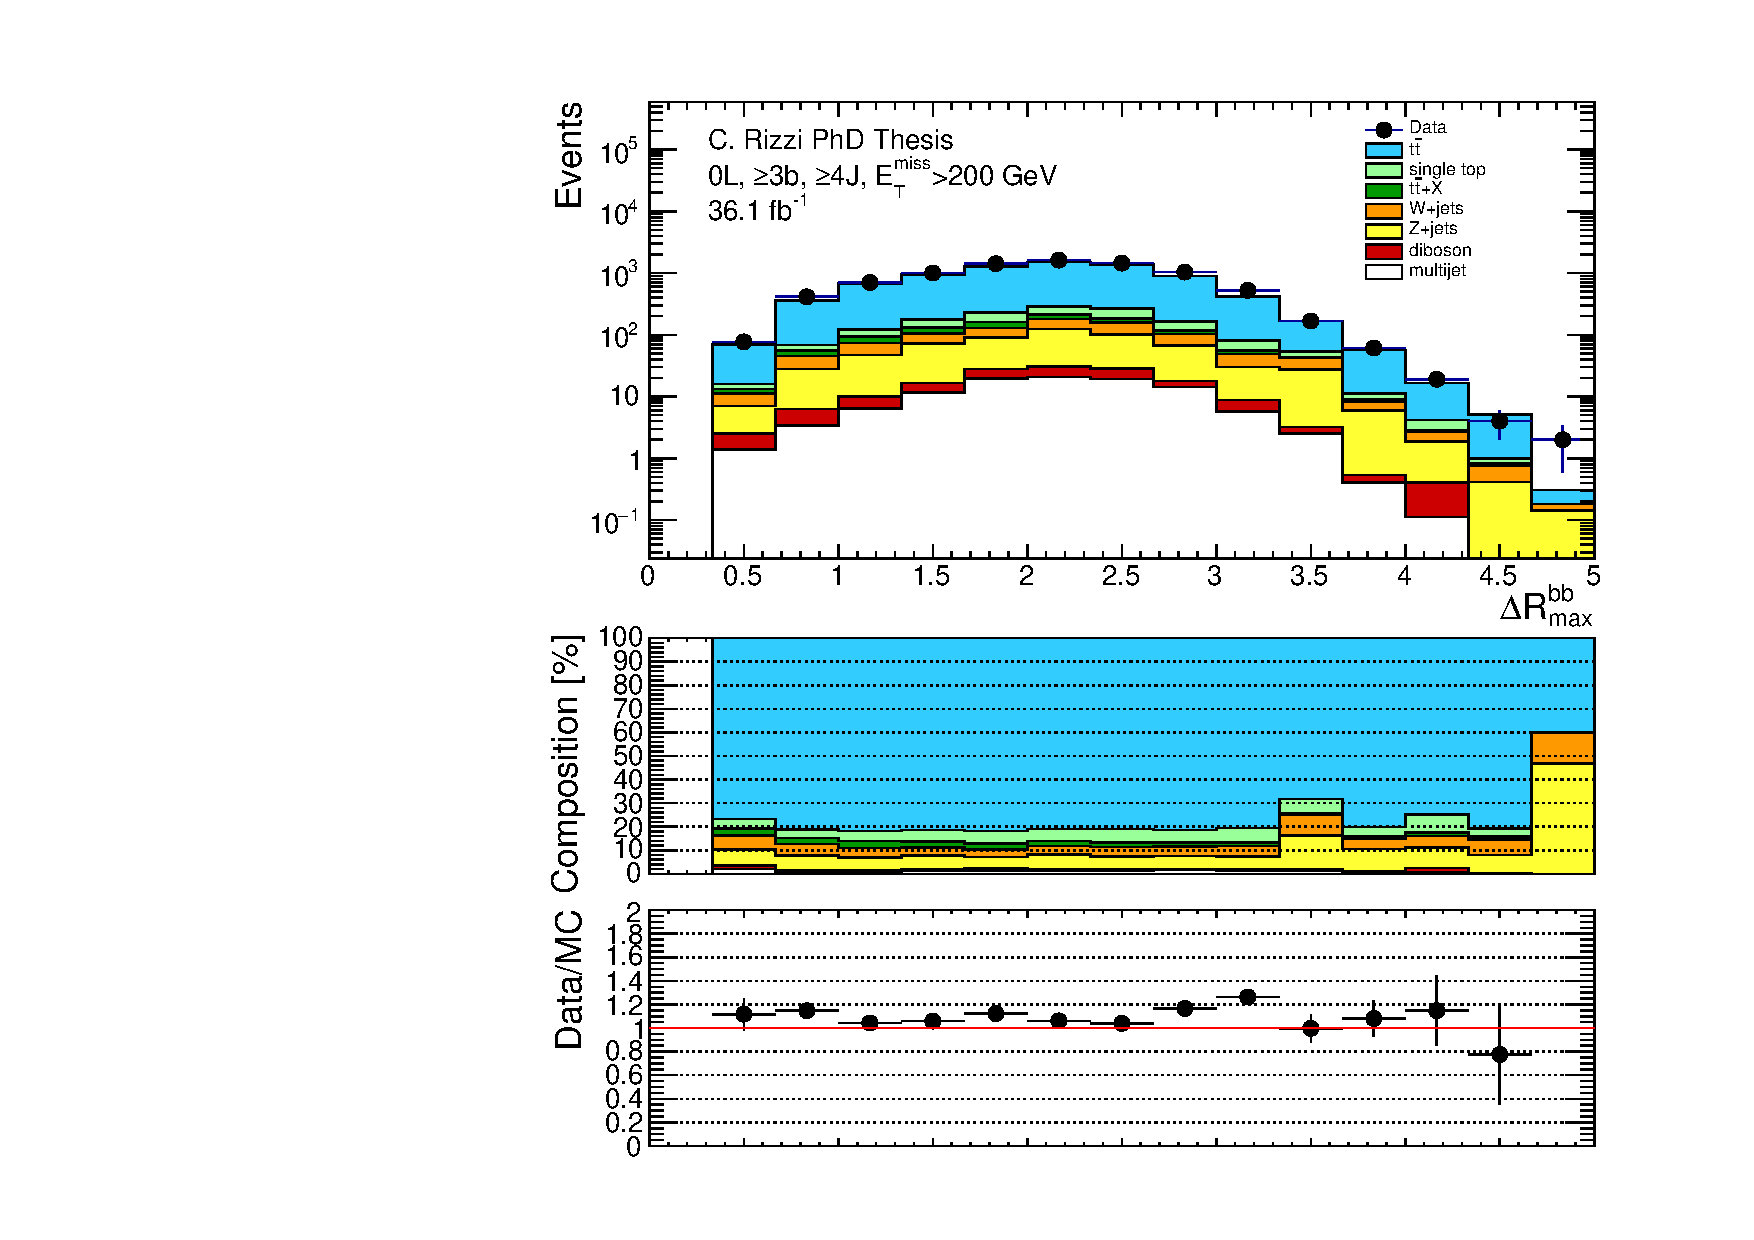
\includegraphics[width=0.45\textwidth]{figures/ewk_prod/data_mc/0L_3bin/data_mc_dRmax_dR.pdf}
\label{fig:ewk:datamc:dRmax_dR}}
\subfigure[\meffb]{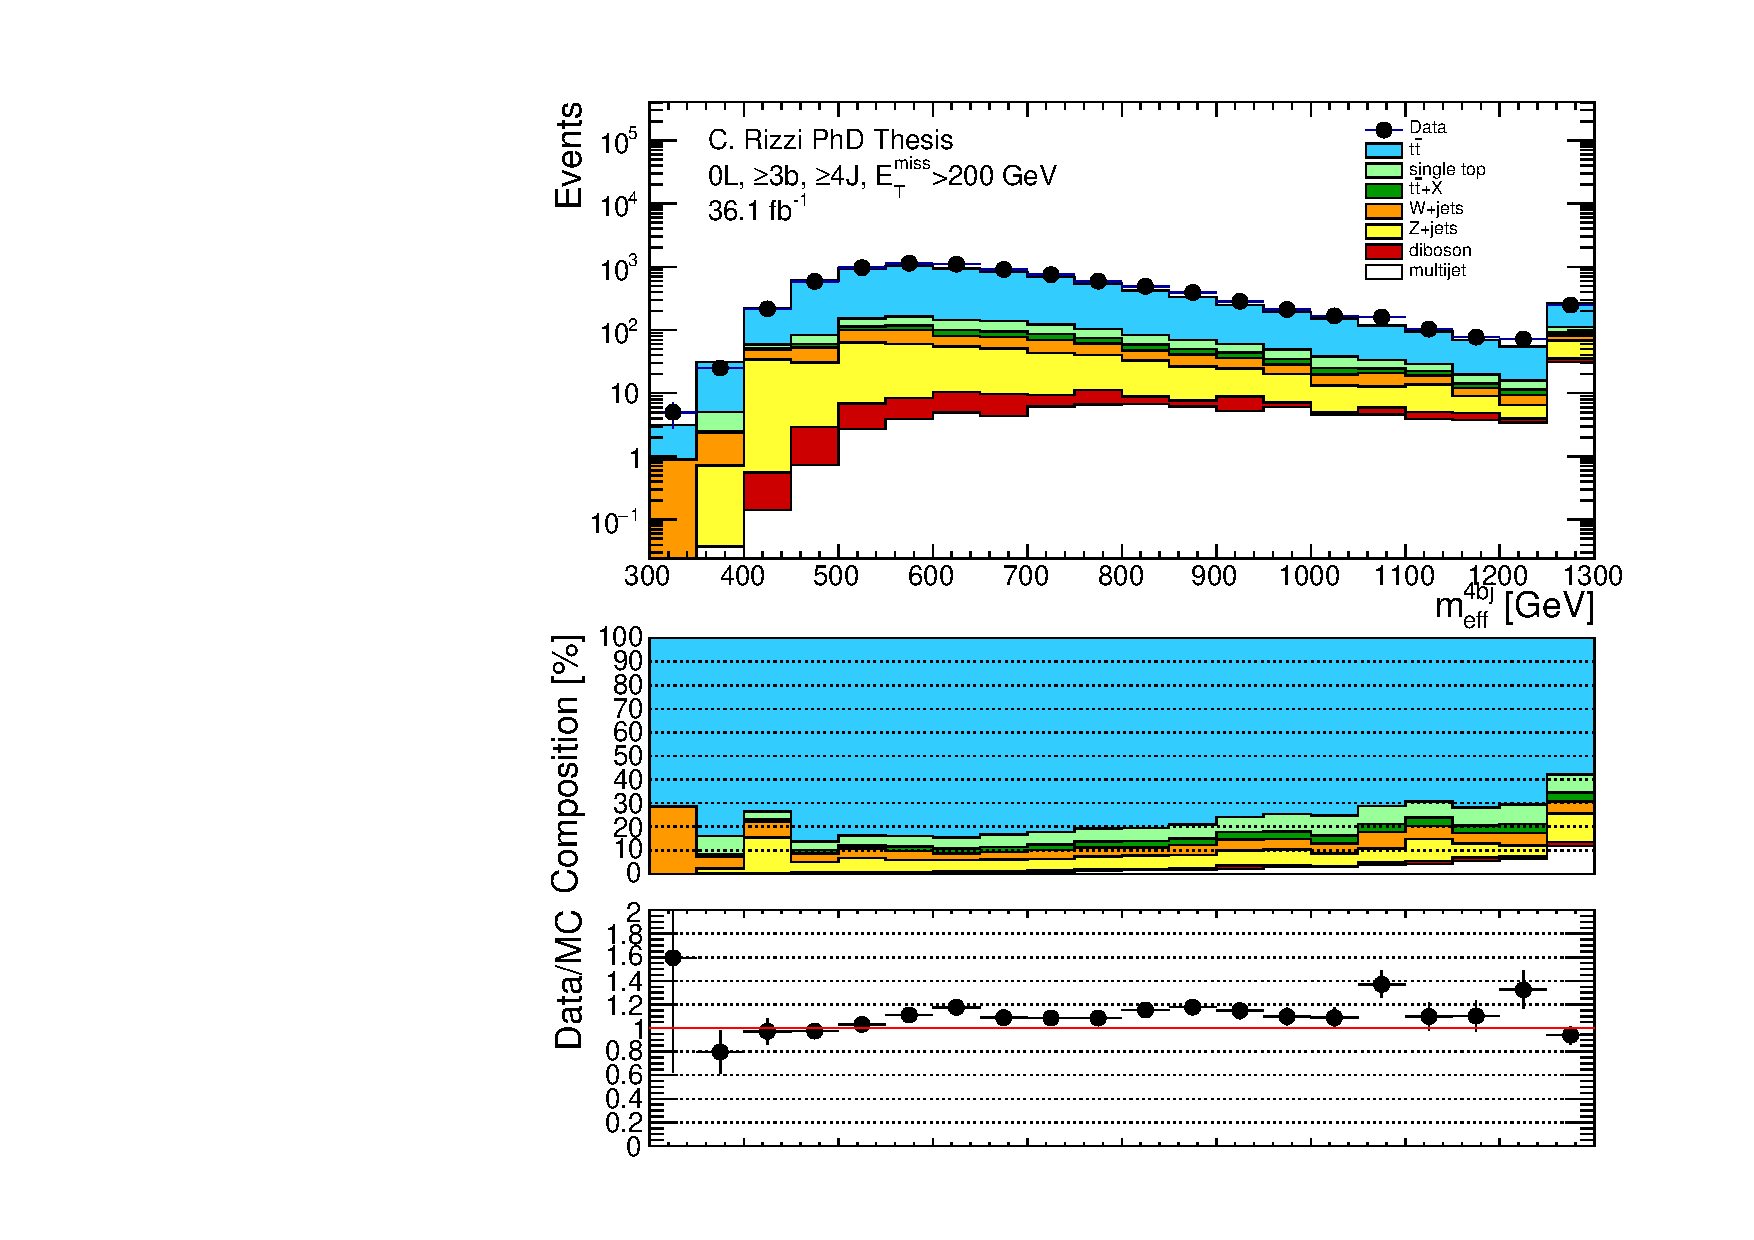
\includegraphics[width=0.45\textwidth]{figures/ewk_prod/data_mc/0L_3bin/data_mc_meff_4bj.pdf}
\label{fig:ewk:datamc:pt_meff_4bj}}
\caption{Comparison between data and simulation in the preselection described in the text.
}
\label{fig:ewk:datamc_a}
\end{figure*}

\clearpage



\section{Systematic Uncertainties}
\label{sec:ewk:syst}

The effect of the systematic uncertainties discussed in Sections \ref{sec:common_syst} and \ref{sec:common_backgrounds} 
is summarized in Figure \ref{fig:syst_etmiss}, showing the relative size of each group of systematics after the fit in the 
\glspl{cr}. 
The meaning of each group of systematics is the same as discussed for the strong-production analysis in Section \ref{sec:strong:syst}.


% \gls{jes} (that has a relative impact on the expected background between 4 and 35\% in the different \glspl{sr}), \gls{jer} (0-26\%) and the uncertainties on the b-tagging efficiency and mistagging rate (3-24\%).
%  \ttbar background, whose impact ranges between 5 and 76\%).

\begin{figure}[htbp]
	\centering
	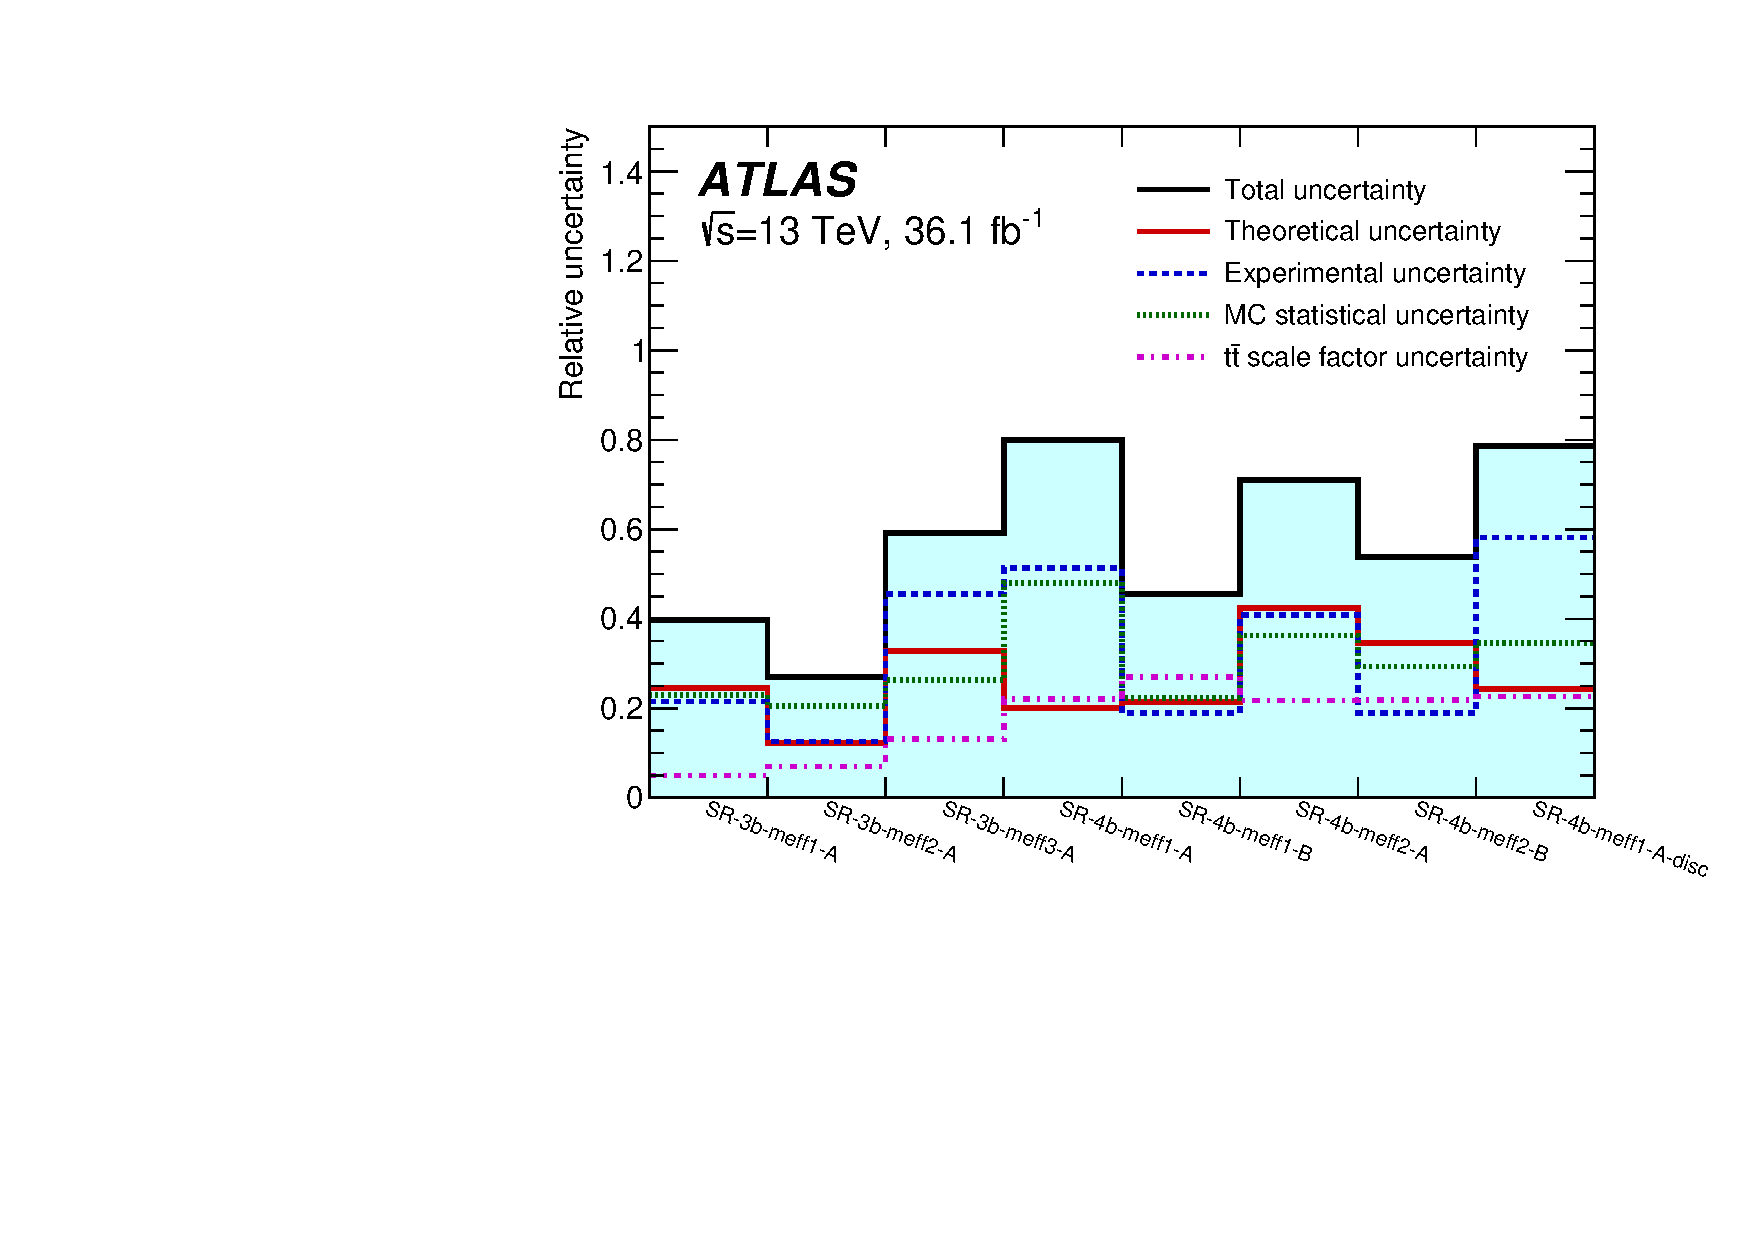
\includegraphics[width=0.85\textwidth]{figures/ewk_prod/etmiss_misc/High-MET-syst.pdf}
	\caption{Relative systematic uncertainties in the background estimate for the high-mass analysis. The individual uncertainties can be correlated, such that the total background uncertainty is not necessarily their sum in quadrature. 
	} 
	\label{fig:syst_etmiss}
\end{figure}

\section{Results}
\label{sec:ewk:results}

Figure \ref{fig:ewk:pullCR} shows the comparison between data and simulation in the \glspl{cr} before the fit (top panel)
and the scale factor for the \ttbar background that is derived from the fit in the \glspl{cr} (bottom panel).
If we compare with the equivalent result for the strong production analysis, in Figure \ref{fig:pullCR}, it is possible 
to see that on average the \ttbar scale factors have values closer to one. 
This is again because of the improvement in the $b$-tagging calibration of $c$-jets was implemented in this analyses. 
The fit in the \glspl{cr} is extrapolated to the \glspl{vr} and to the \glspl{sr}. 

The post-fit data-\gls{mc} agreement in the \glspl{vr} is shown in Figure \ref{fig:ewk:pullVR}: the top panel of this figure 
shows the post-fit predicted yields in each of the \glspl{vr} and the data yields, while the bottom panel quantifies the 
difference between observed data and predictions in terms of the significance, defined as in Ref. \cite{Choudalakis:2011okv}. 
Note that this is different from the pull definition adopted in Figure \ref{fig:pullVR}. 
The closure in the \glspl{vr} is good: all the bins have discrepancies with significance lower than 0.8. 

The results in the \glspl{sr} are shown in Figure \ref{fig:ewk:pullSR}. As in Figure \ref{fig:ewk:pullVR}, the top panel shows the 
predicted and observed yields in each \gls{sr}, and the bottom panel the significance of the discrepancy. 
No significant excess is observed and the observations are in agreement with the \gls{sm} predictions. 
The numerical results of the background-only fit extrapolated to the \glspl{sr} are presented also in Table \ref{tab:ewk:yieldsSR},
where the background prediction is also broken down by component. 
This table shows also the total background prediction before the fit in the \glspl{cr}, which is labeled ``MC-only background''.


\begin{figure}[htbp]
	\centering
	\includegraphics[width=0.9\textwidth]{figures/ewk_prod/etmiss_results/histpull_pulls_in_CR_qcdStrong}
	\caption{Event yields in control regions and related \ttbar\
          normalization factors after the background-only fit for
          %Inputs and results of the likelihood fit in the control
          %regions of
          the high-mass analysis. The upper panel shows 
		the observed number of events and the predicted background yield before the fit.
		All uncertainties  shown in Figure \ref{fig:syst_etmiss} are included in the uncertainty band. The background category $\ttbar+X$ includes $\ttbar W/Z$, $\ttbar H$, and $\ttbar \ttbar$ events.  
		The $\ttbar$ normalization is obtained from the fit
                and is displayed in the bottom panel. Figure from Ref. \cite{Aaboud:2018htj}.
	} 
	\label{fig:ewk:pullCR}
\end{figure}


\begin{figure}[htbp]
	\centering
	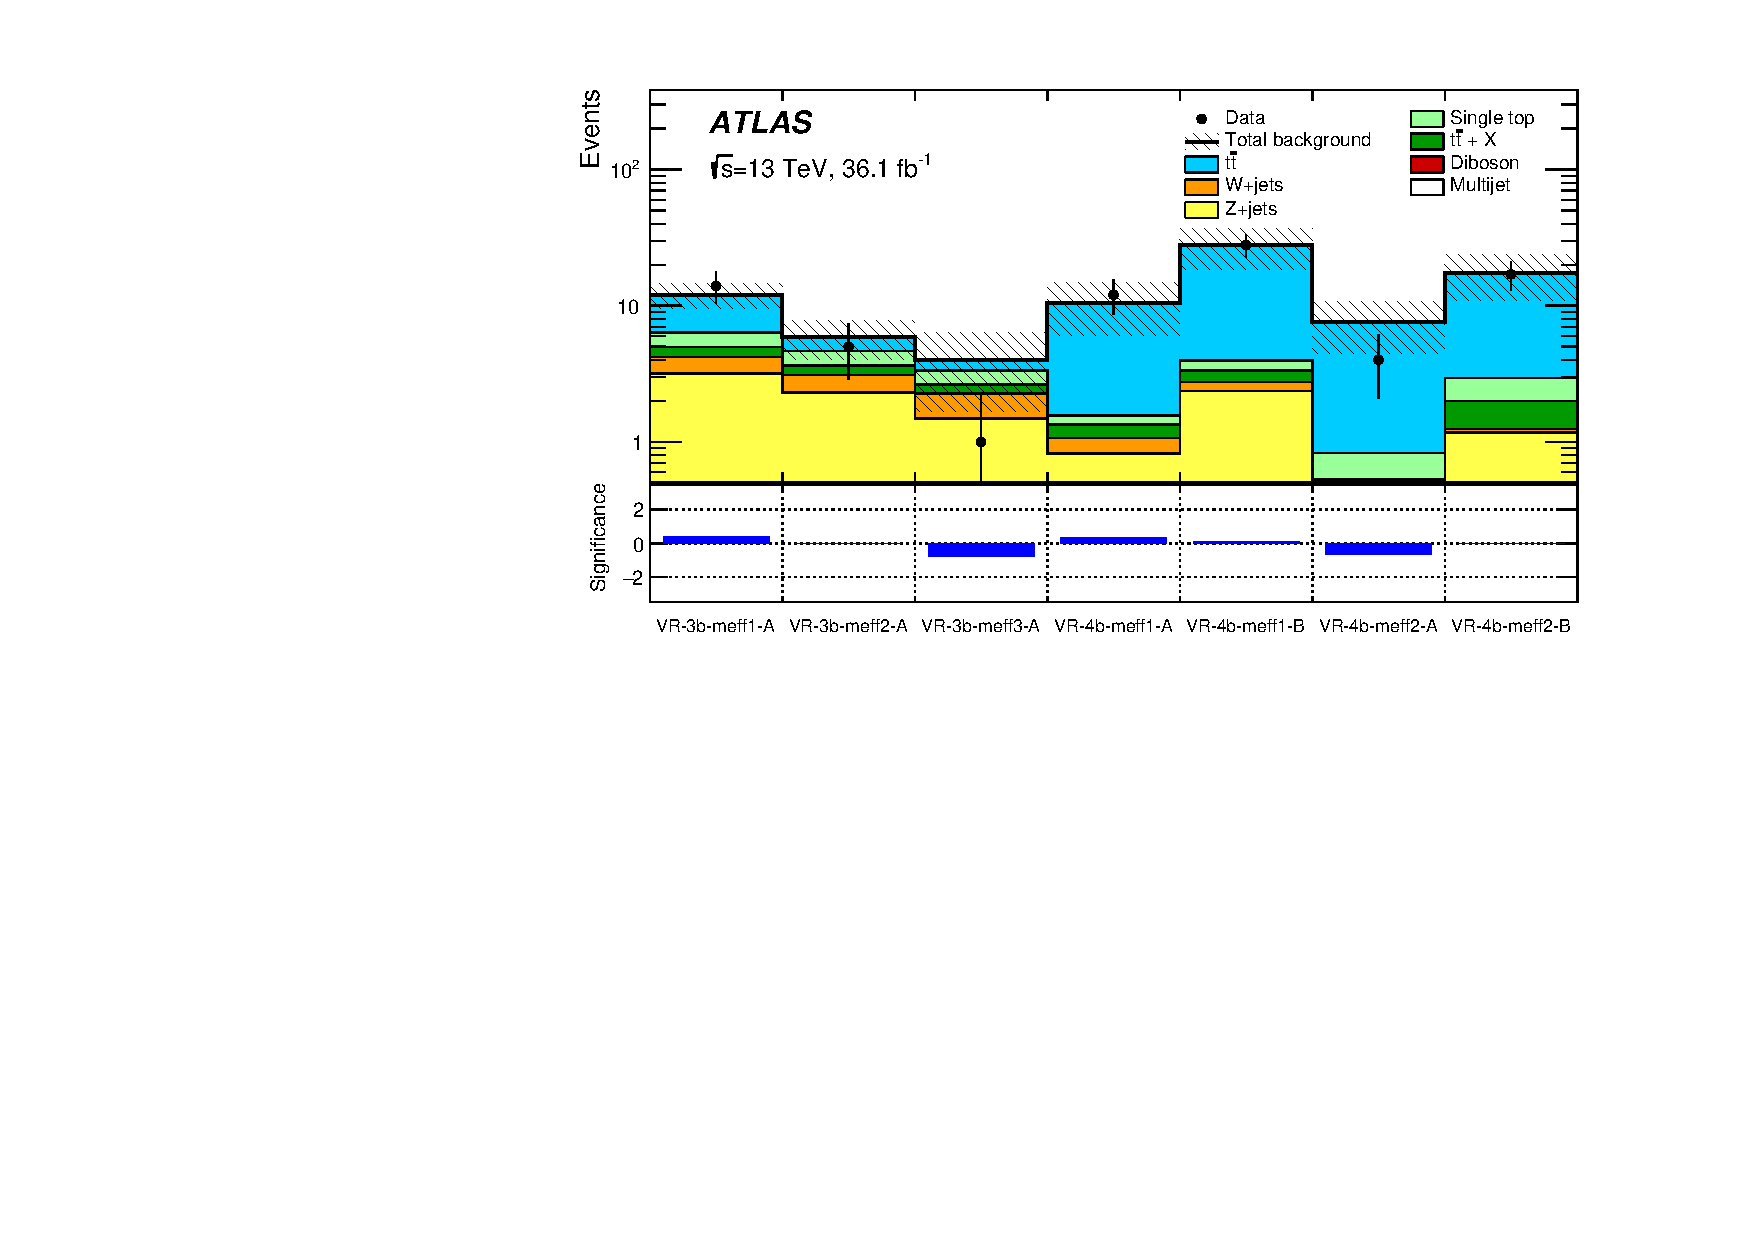
\includegraphics[width=0.9\textwidth]{figures/ewk_prod/etmiss_results/histpull_pulls_in_VR_qcdStrong}
	\caption{Results of the background-only fit extrapolated to the \glspl{vr}. 
	    The $\ttbar$ normalization is obtained from the fit to the \glspl{cr} shown in Figure~\ref{fig:ewk:pullCR}. The upper panel shows 
		the observed number of events and the predicted background yield. The bottom panel shows the significance of any disagreement between the data and the background model, computed as in Ref. \cite{Choudalakis:2011okv}.
		All uncertainties  shown in Figure \ref{fig:syst_etmiss} are included in the 
		uncertainty band. The background category $\ttbar+X$ includes $\ttbar W/Z$, 
		$\ttbar H$, and $\ttbar \ttbar$ events. Figure from Ref. \cite{Aaboud:2018htj}.}
	\label{fig:ewk:pullVR}
\end{figure}

\begin{figure}[htbp]
	\centering
	% \subfigure[]{\includegraphics[width=0.65\textwidth]{figures/etmiss_results/histpull_pulls_in_CR_qcdStrong}\label{fig:pullCR}}\\
	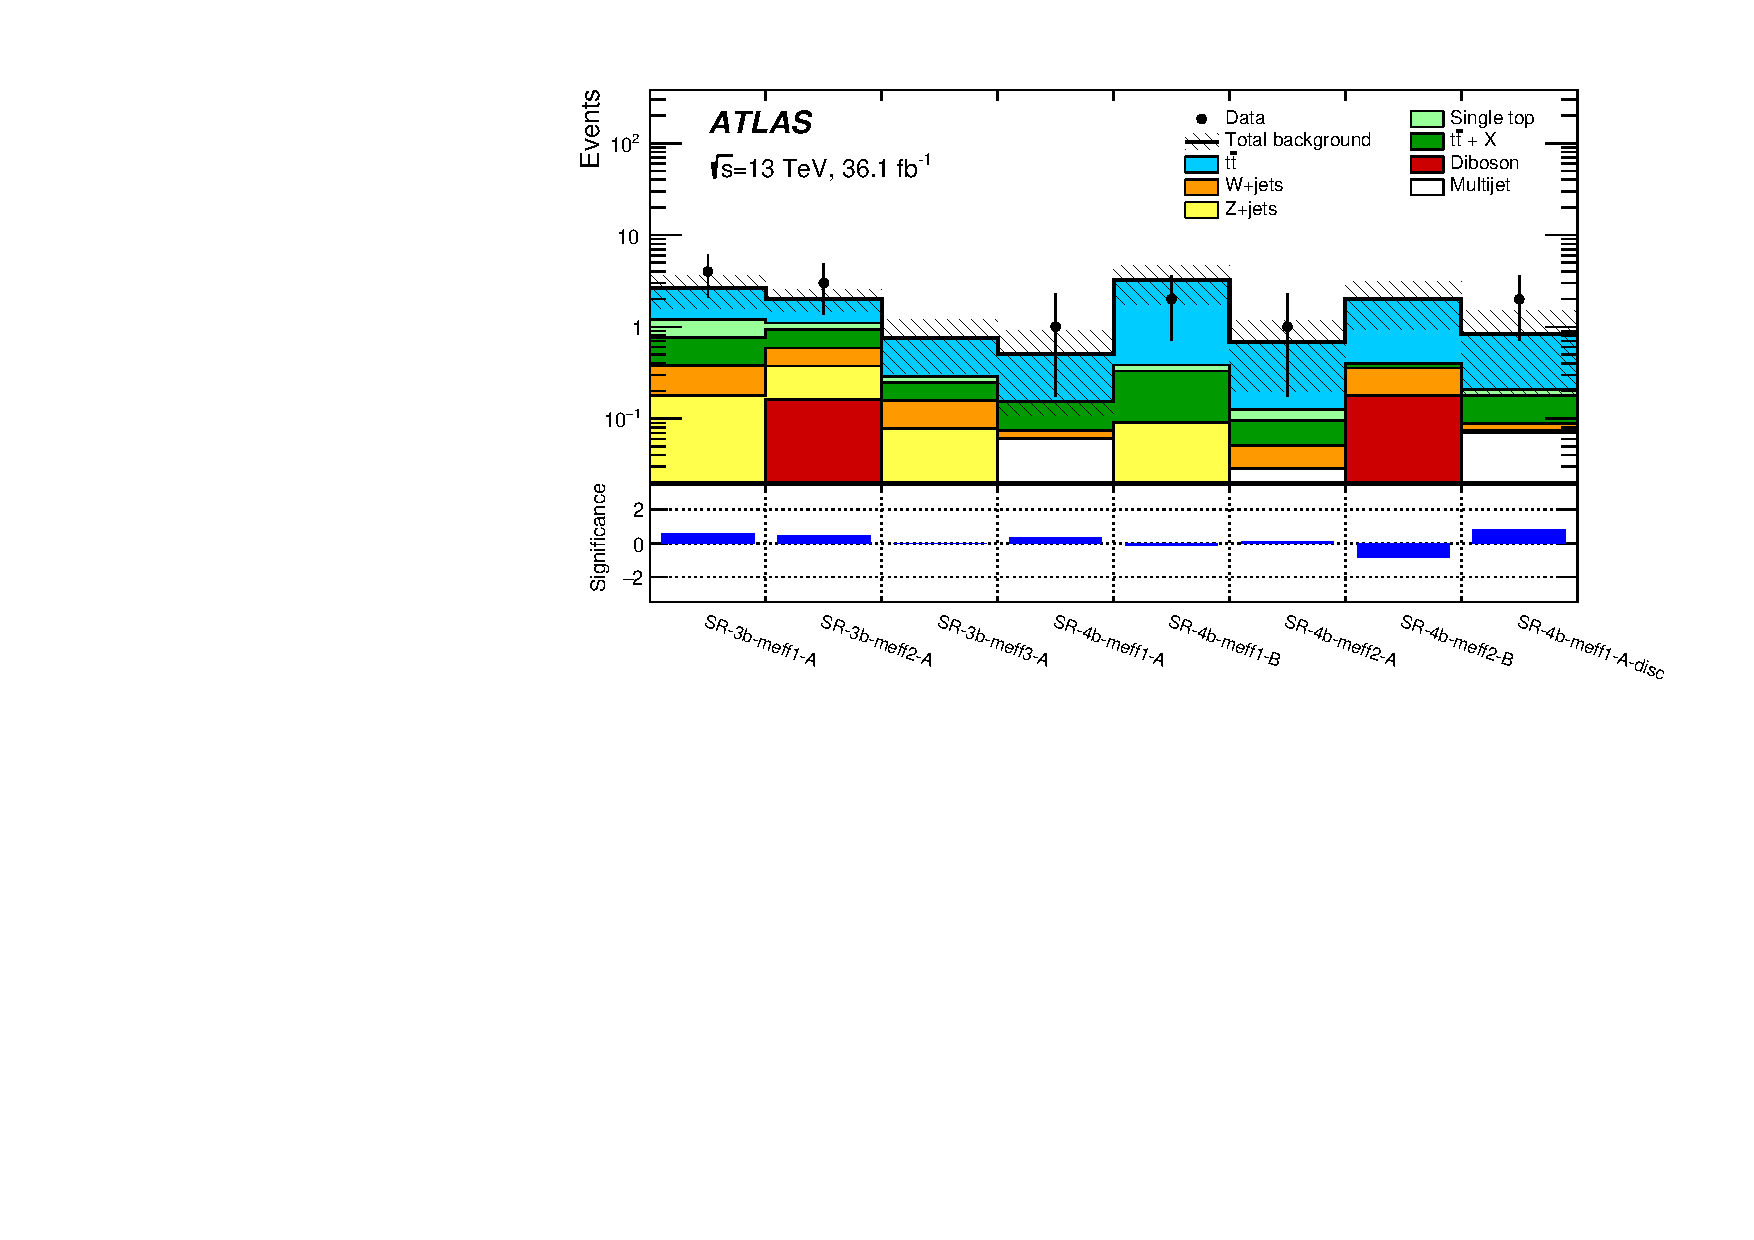
\includegraphics[width=0.9\textwidth]{figures/ewk_prod/etmiss_results/histpull_pulls_in_SR_qcdStrong}
	\caption{Results of the background only fit extrapolated to the \glspl{sr}. 
	The $\ttbar$ normalization is obtained from the fit to the CRs shown in Figure~\ref{fig:pullCR}. The data in the  SRs are 
	not included in the fit.  The upper panel shows the observed number of events and the predicted background 
	yield.  The bottom panel shows the significance of any disagreement between the data and the background model, computed as in Ref. \cite{Choudalakis:2011okv}. All uncertainties  shown in Figure \ref{fig:syst_etmiss} are included in the uncertainty band. 
	The background
	category $\ttbar+X$ includes $\ttbar W/Z$, $\ttbar H$, and $\ttbar \ttbar$ events. Figure from Ref. \cite{Aaboud:2018htj}.} 
	\label{fig:ewk:pullSR}
\end{figure}

\begin{table}
%\resizebox{1.\textwidth}{!}{
\renewcommand{\arraystretch}{1.1}
\begin{tabular}{l|c|c|c|c}
\toprule
SR name & SR-3b-meff1-A & SR-3b-meff2-A & SR-3b-meff3-A & SR-4b-meff1-A \\
\hline
$N_{\mathrm{obs}}$ & 4 & 3 & 0 & 1 \\
\hline
Total background & 2.6 $\pm$ 1.0 & 2.0 $\pm$ 0.5 & 0.8 $\pm$ 0.5 & 0.5 $\pm$ 0.4  \\
Fitted \ttbar & 1.4 $\pm$ 0.8 & 0.89 $\pm$ 0.32 & 0.5 $\pm$ 0.4 & 0.35 $\pm$ 0.33 \\

Single top & 0.43 $\pm$ 0.29 & 0.17 $\pm$ 0.14 & 0.040 $\pm$ 0.017 & $<$ 0.01 \\
$\ttbar+X$ & 0.39 $\pm$ 0.16 & 0.34 $\pm$ 0.14 & 0.09 $\pm$ 0.04 & 0.08 $\pm$ 0.06  \\
$Z$+jets & 0.18 $\pm$ 0.14 & 0.21 $\pm$ 0.16 & 0.07 $\pm$ 0.20 & $<$ 0.01 \\
$W$+jets & 0.20 $\pm$ 0.06 & 0.21 $\pm$ 0.09 & 0.08 $\pm$ 0.06 & 0.013 $\pm$ 0.009  \\
Diboson & $<$ 0.01 & 0.16 $\pm$ 0.11 & $<$ 0.01 & $<$ 0.01 \\
Multijet & $<$ 0.01 & 0.004 $\pm$ 0.005 & 0.004 $\pm$ 0.006 & 0.06 $\pm$ 0.05 \\
\hline
MC-only background & 2.5 $\pm$ 1.0 & 2.0 $\pm$ 0.5 & 0.6 $\pm$ 0.4 & 0.43 $\pm$ 0.31 \\
\bottomrule
\end{tabular}

\vspace{0.4cm}

\begin{tabular}{l|c|c|c|c}
\toprule
SR name & SR-4b-meff1-B & SR-4b-meff2-A & SR-4b-meff2-B & SR-4b-meff1-A-disc\\
\hline
$N_{\mathrm{obs}}$ & 2 & 1 & 0 & 2\\
\hline
Total background &  3.2 $\pm$ 1.5 & 0.7 $\pm$ 0.5 & 2.0 $\pm$ 1.1 & 0.8 $\pm$ 0.7\\
Fitted \ttbar &  2.8 $\pm$ 1.5 & 0.6 $\pm$ 0.5 & 1.6 $\pm$ 1.0 & 0.6 $\pm$ 0.6\\
Single top &  0.06 $\pm$ 0.13 & 0.030 $\pm$ 0.019 & $<$ 0.01 & 0.030 $\pm$ 0.019\\
$\ttbar+X$ & 0.24 $\pm$ 0.10 & 0.045 $\pm$ 0.025 & 0.039 $\pm$ 0.033 & 0.09 $\pm$ 0.06\\
$Z$+jets &  0.09 $\pm$ 0.04 & $<$ 0.01 & $<$ 0.01 & 0.004 $\pm$ 0.011\\
$W$+jets & $<$ 0.01 & 0.022 $\pm$ 0.027 & 0.18 $\pm$ 0.10 & 0.013 $\pm$ 0.008\\
Diboson &  $<$ 0.01 & $<$ 0.01 & 0.17 $\pm$ 0.08 & $<$ 0.01\\
Multijet &  0.0027 $\pm$ 0.0021 & 0.03 $\pm$ 0.04 & 0.007 $\pm$ 0.012 & 0.07 $\pm$ 0.05\\
\hline
MC-only background & 2.6 $\pm$ 0.9 & 0.43 $\pm$ 0.27 & 1.3 $\pm$ 0.6 & 0.7 $\pm$ 0.5\\
\bottomrule
\end{tabular}
%} 
\caption{Results of the background-only fit extrapolated to the SRs of the high-mass analysis, for the total background prediction and breakdown of the main background sources. 
	The uncertainties shown include all systematic uncertainties. The data in the SRs are not included in the fit. 
	The background category $\ttbar+X$ includes $\ttbar W/Z$, $\ttbar H$, and $\ttbar \ttbar$ events.
	The row ``MC-only background'' provides the total background prediction when the
	$\ttbar$ normalization is obtained from a theoretical
	calculation~\cite{Czakon:2011xx}. Table from Ref. \cite{Aaboud:2018htj}.}
\label{tab:ewk:yieldsSR}
\end{table}




\FloatBarrier

\section{Interpretation}
\label{sec:ewk:interp}

The results presented in Section \ref{sec:ewk:results} are used to set limits on the presence of \gls{bsm} signals.

\subsection{Model-independent limits}
\label{sec:ewk:modelindepUL}

The number of expected and observed events in the two discovery \glspl{sr} SR-4b-meff1-A-disc and SR-3b-meff3-A are used to set model-independent limits on the number of \gls{bsm} events. 
These limits, obtained with the \gls{cls} procedure, ignore any signal contamination in the \glspl{cr} and are reported in Table \ref{tab:ewk:UL_toys}.
In the same table are reports also the model-independent limits obtained from the low-mass analysis, complementary to the analysis 
discussed in this thesis, which is briefly presented in Section \ref{sec:ewk:LM}. 
To distinguish them from the ones of the low-mass analysis, the results in SR-4b-meff1-A-disc and SR-3b-meff3-A are labeled as 
high-SR-4b-meff1-A-disc and high-SR-3b-meff3-A respectively. 

\begin{table}
\begin{center}
\begin{tabular}{
      lr
      S[table-format=4.1(1)]
      S[table-format=1.1(2)]
      S[table-format=2.1(1)]
      cc
      }
\toprule
{ Signal channel}           &   $N_\mathrm{obs}$ & \multicolumn{1}{c}{$N_\mathrm{pred}$}       & \multicolumn{1}{c}{$\sigma^\mathrm{95}_\mathrm{vis}$ [fb]}  &  $S_\mathrm{obs}^\mathrm{95}$  & $S_\mathrm{exp}^\mathrm{95}$ & $p_0$ (Z)  \\
\midrule
high-SR-4b-meff1-A-disc   &    2 &     0.8 $\pm$ 0.7  & 0.15 &   5.5 & ${ 4.2 }^{ +1.3 }_{ -0.4 }$  &  0.15$~$(1.02) \\%
high-SR-3b-meff3-A        &    0 &     0.8 $\pm$ 0.5  & 0.08 &   3.0 & ${ 3.1 }^{ +1.2 }_{ -0.1 }$  &  0.50$~$(0.00) \\%
low-SR-MET0-meff440       & 1063 &    1100 $\pm$ 25   & 2.3  &  56   & ${ 79 }^{ +31 }_{ -23 }$     &  0.50$~$(0.00) \\%
low-SR-MET150-meff440     &   17 &      12 $\pm$ 8    & 0.90 &  22   & ${ 19 }^{ +5 }_{ -4 }$       &  0.21$~$(0.80) \\%
\bottomrule
\end{tabular}
\end{center}
\caption[Model independent upper limits]{For each discovery region, the number of observed events ($N_\mathrm{obs}$), the number of predicted events ($N_\mathrm{pred}$), and 95\% CL upper limits on the visible cross-section ($\sigma^\mathrm{95}_\mathrm{vis}$) and on the number of signal events ($S_\mathrm{obs}^\mathrm{95}$ ) are shown.  The fifth column ($S_\mathrm{exp}^\mathrm{95}$) shows the 95\% CL upper limit on the number of signal events given the expected number (and $\pm 1\sigma$ excursions of the expectation) of background events. The last column indicates the discovery $p$-value ($p(s=0)$) in significance units. The $p$-values are capped at 0.5. Results are obtained with $20\,000$ pseudoexperiments.
Table from Ref. \cite{Aaboud:2018htj}.
}
\label{tab:ewk:UL_toys}
\end{table}

\subsection{Model-dependent limits}
\label{sec:ewk:modeldep}

A combined fit that includes simultaneously all the \glspl{cr} and all the orthogonal \glspl{sr} (i.e. all the \glspl{sr}
except from  SR-4b-meff1-A-disc) is used to place limits on the specific models described in Section \ref{sec:ewk:sig}.

The signal model that is used to optimize the analysis regions is higgsino pair production with $B(\hino\rightarrow h \tilde{G})=100$\%.
The 95\% upper limits on the total pair production cross-section for this model is shown in Figure \ref{fig:exclusion_high}, 
as a function of \mhino. 
The expected exclusion is between 250 and 830 GeV in \mhino. 
Due to the slight deficit in the region with the highest \meffb selection, the observed exclusion is up to 880 GeV.

A second interpretation of the results is provided in Figure \ref{fig:exclusion_high:BR}, showing the exclusion contour in the 
plane $B(\hino\rightarrow h \tilde{G})$-\mhino, with the assumption $B(\hino\rightarrow h \tilde{G}) + B(\hino\rightarrow Z \tilde{G}) =1$.
For $\mhino = 400$ GeV, which is the mass point with the lowest excluded $\sigma/\sigma_{\rm theory}$, we exclude at 95\% \gls{cl}
\glspl{br} as low as 45\%.


\begin{figure}[htbp]
	\centering
	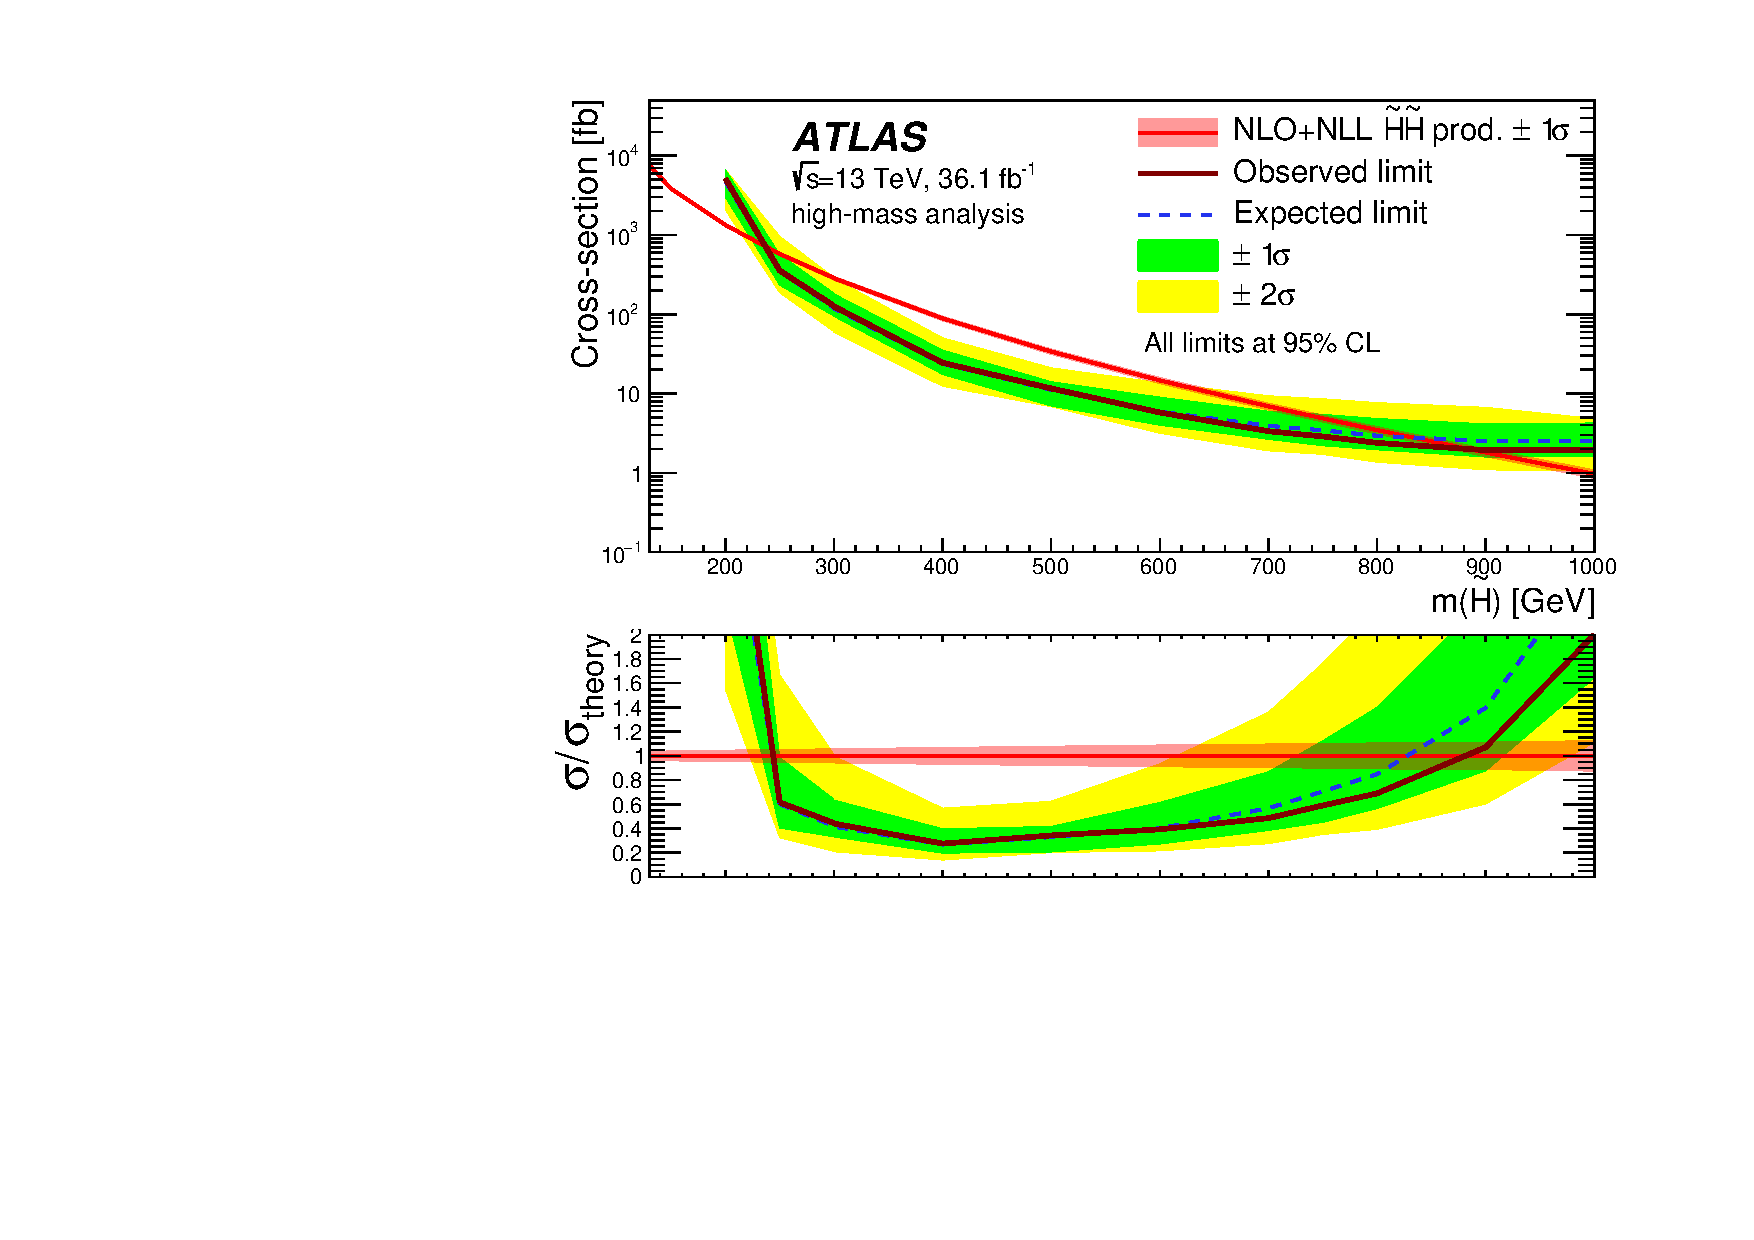
\includegraphics[width=0.8\textwidth]{figures/ewk_prod/interpretation/limit_HM}
	\caption{The observed (solid black) vs expected (dashed black) 95\% upper limits on the total pair production cross-section for degenerate higgsinos as a function of \mhino. The 1 and 2$\sigma$ uncertainty bands are shown as green and yellow, respectively. The theory cross-section is shown in the red curve. The bottom panel shows the ratio of the observed and expected limits with the theory cross-section. Figure from Ref. \cite{Aaboud:2018htj}.} 
	\label{fig:exclusion_high}
\end{figure}

\begin{figure}[htbp]
	\centering
	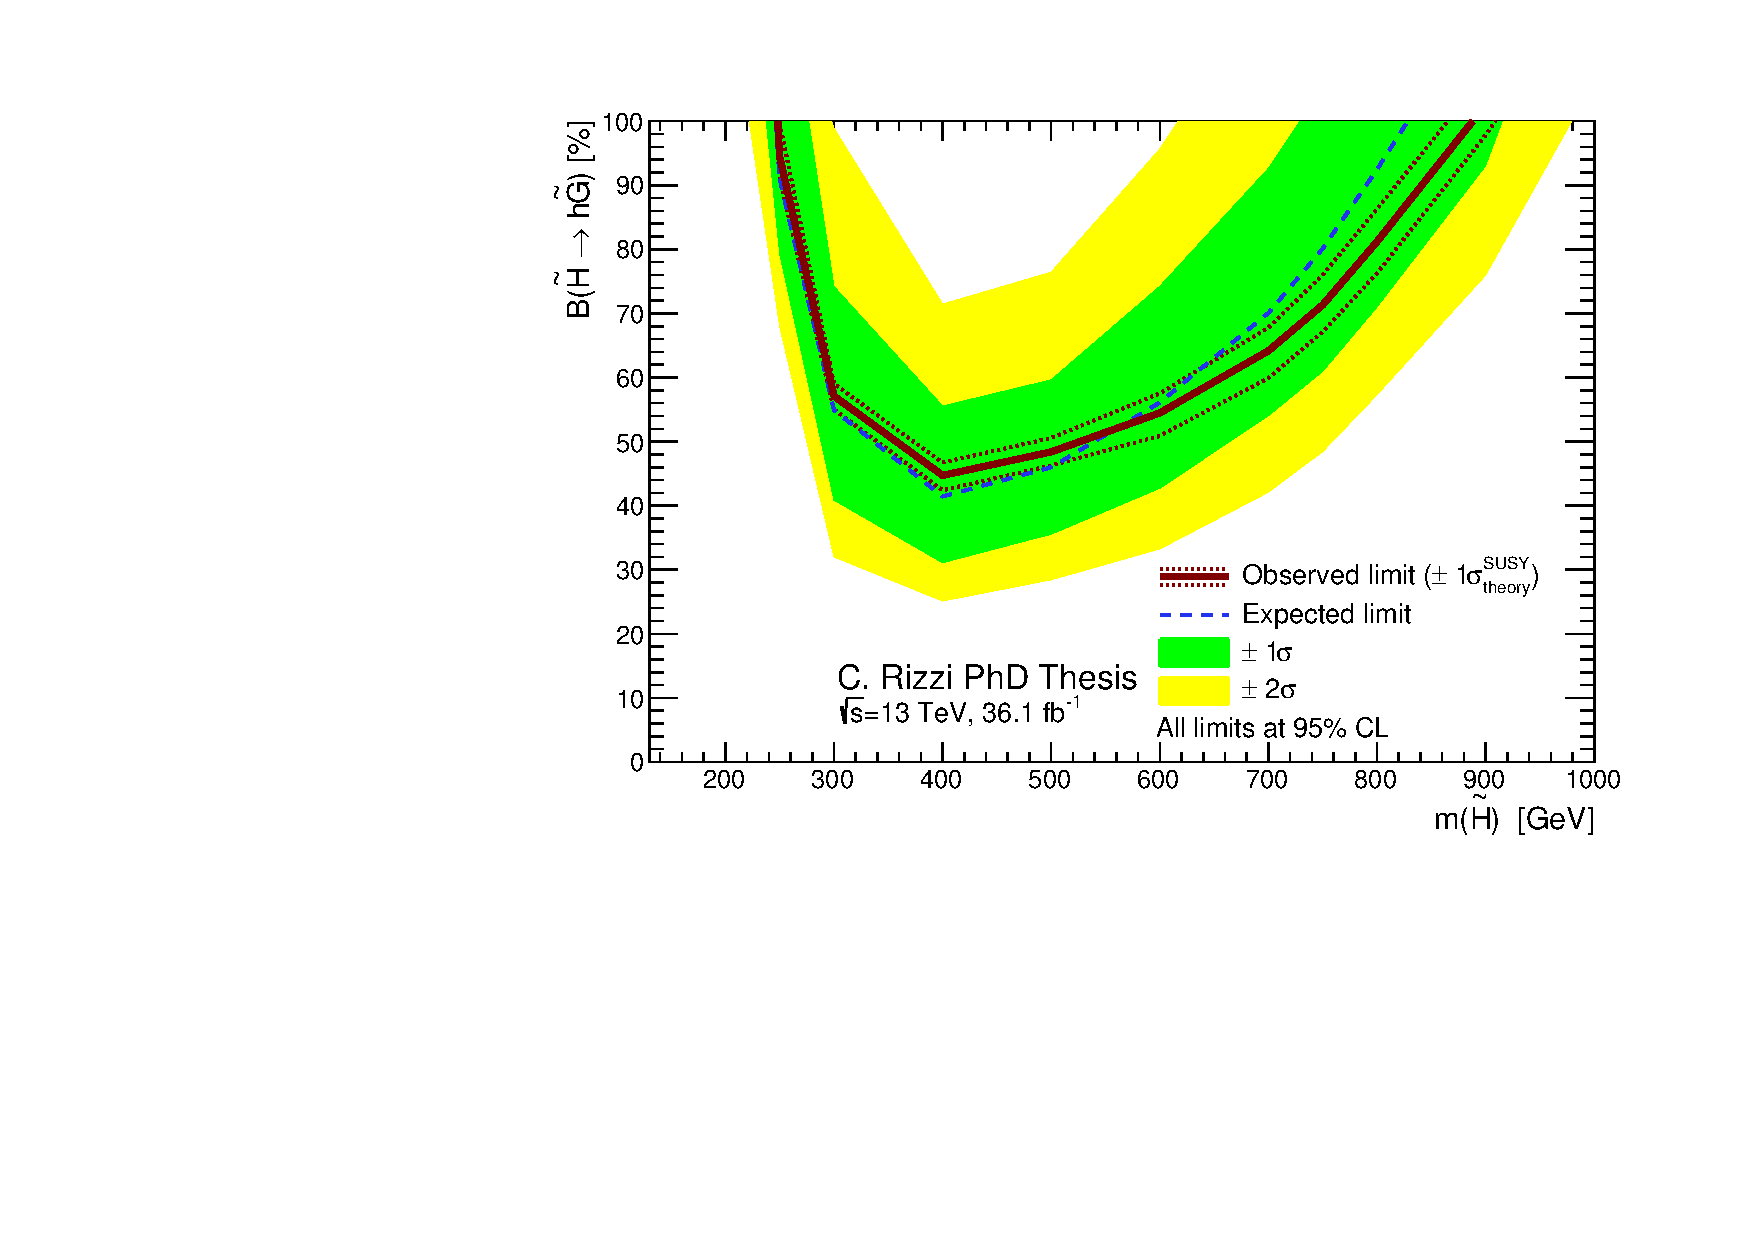
\includegraphics[width=0.8\textwidth]{figures/ewk_prod/interpretation/br_limit_HM.pdf}
	\caption{The observed (solid) vs expected (dashed) 95\% limits in the \mhino\ vs $B(\hino\rightarrow h \tilde{G})$ plane, where $B(\hino\rightarrow h \tilde{G})$ denotes the branching ratio for the decay $\hino \rightarrow h \gravino$. The 1$\sigma$ uncertainty band is overlaid in green and the 2$\sigma$ in yellow. The regions above the lines are excluded by the analysis.} 
	\label{fig:exclusion_high:BR}
\end{figure}

\FloatBarrier



\section{Complementary low-mass higgsino search}
\label{sec:ewk:LM}

The analysis discussed in this chapter is limited in sensitivity for low \mhino, as it is clear from Figure \ref{fig:exclusion_high}. 
This is because when \mhino approaches the Higgs mass, the decay products (Higgs boson and \gravino)
have increasingly low \pt, and a low \pt \gravino does not produce enough \met to satisfy the \met trigger requirements and be selected 
in the analysis. 
To gain sensitivity also to the low-\mhino part of the mass spectrum, which is particularly interesting for Naturalness arguments (see the 
discussion in Section \ref{sec:theo:naturalsusy}), 
this analysis is complemented by a second analysis that targets low-\met events, referred to as "low-mass" analysis \cite{Aaboud:2018htj}. 
Events are selected using $b$-jet triggers and are required to have at least four $b$-tagged jets, 
using a $b$-tagging \gls{op} with an efficiency of 70\%
(tighter than the 77\% used in the high-mass analysis).
This analysis uses data from 2016 where the $b$-jet triggers are available, corresponding to an integrated luminosity of 24.3 \ifb.

The jets used to reconstruct the Higgs candidates are the four with the highest $b$-tagging score, and are paired minimizing the quantity 
$D_{hh}$, defined as:
\begin{equation}
  D_{hh} = \left|m_{2j}^\textrm{lead} - \frac{120}{110}m_{2j}^\textrm{subl}\right| \; ,
\end{equation}
where $m_{2j}^\textrm{lead}$ and $m_{2j}^\textrm{subl}$ are the masses of the Higgs boson candidates with leading and subleading \pt respectively.
This pairing choice tends to create two Higgs candidates with similar mass; 
for low higgsino masses the $b$-jets originating form the decay of the Higgs bosons are less collimated, 
and this choice is therefore more effective than minimizing \dRmax. 

The main background is constituted by multijet events and a small fraction of \ttbar events, as opposed to the
high mass analysis, where multijet is an almost-negligible background after applying the \dphimin selection. 
The background from \ttbar events is further reduced by requiring $X_{Wt}>1.8$, defined as:

\begin{equation}
 X_{Wt} = \sqrt{\left( \frac{m_W - 80.4\,\ \gev}{0.1  m_W} \right)^2 + \left( \frac{m_t - 172.5\,\ \gev}{0.1  m_t} \right)^2 } \;,
\label{eqn:xwt}
\end{equation}

\noindent where the top and W-boson candidates are built as described in Ref. \cite{Aaboud:2018htj}. 
A low value of $X_{Wt}$ corresponds to a high probability of the event to be a \ttbar event. 

The \gls{sr} is defined by requiring: 
\begin{equation}
X_{hh}^\textrm{SR} = \sqrt{ \left( \frac{m_{2j}^\textrm{lead} - 120\ \gev}{0.1 m_{2j}^\textrm{lead}} \right)^2 + \left( \frac{m_{2j}^\textrm{subl} - 110\ \gev}{0.1 m_{2j}^\textrm{subl}} \right)^2} \ <\ 1.6,
\end{equation}
\noindent where $0.1  m_{2j}^\textrm{lead}$ and $0.1 m_{2j}^\textrm{subl}$ approximate the mass resolution of the two Higgs 
boson candidates. 

The events in the \gls{sr} are further binned based on the two-dimensional distribution of \met and \meff, 
and this is used as input in the statistical analysis. The binning used is:
\begin{eqnarray*} 
\met &=& \{0, 20, 45, 70, 100, 150, 200\} \;, \\
\meffb &=&\{160, 200, 260, 340, 440, 560, 700, 860\} \;,
\end{eqnarray*}

\noindent where the values are expressed in GeV.

Two dedicated discovery regions have optimized selections to maximize the discovery significance for \mhino = 150 and 300 GeV:
\begin{itemize}
\item low-SR-MET0-meff440: \meffb $>$ 440 GeV.
\item low-SR-MET150-meff440: \meffb $>$ 440 GeV, \met $>$ 150 GeV.
\end{itemize}

The background estimate is fully data-driven and relies on a sample with exactly two $b$-tagged jets (orthogonal to the \gls{sr} and 
with very low signal contamination). $m_{2j}^\textrm{lead}$ and $m_{2j}^\textrm{subl}$ are used to define a \gls{cr} and two \glspl{vr}, both in the $\geq4b$ and in the $2b$ samples; all these regions exclude the $X_{hh}^\textrm{SR}<1.6$ area, to be orthogonal to the \gls{sr}.
The 2-tag and 4-tag \glspl{cr} are used to derive a reweighting function to go from the 2-tag sample to the 4-tag sample, that consists in two steps:
first of all an overall normalization correction is applied, and then 
a reweighting based on boosted decision trees corrects for further kinematic differences. 
This reweighting procedure is tested in the \glspl{vr} and then applied to the \glspl{vr}.
More details on the background estimate and its validation are available in Ref. \cite{Aaboud:2018htj}.

\section{Combined Results}

Figures \ref{fig:ewk:exclusion_comb} and \ref{fig:ewk:exclusion_combBR} show the combined results of the two analyses for the model-dependent 
exclusion, respectively in the case $B(\hino\rightarrow h \tilde{G})=100$\% and in the \mhino vs $B(\hino\rightarrow h \tilde{G})$ plane.
The results of the low-mass analysis are used below 300 GeV, while above it is the high-mass search that provides the nominal result.
The transition at 300 GeV is chosen such that in the transition point the two analyses have 
similar sensitivity in the case $B(\hino\rightarrow h \tilde{G})=100$\%.
In the low-mass analysis the high-\met bins of the \gls{sr} show a mild excess; 
therefore, the observed limit is weaker than expected and the portion of the mass spectrum between 230 and 290 GeV is not excluded in the 
$B(\hino\rightarrow h \tilde{G})=100$\%, despite the expected sensitivity. 

\begin{figure}[htbp]
	\centering
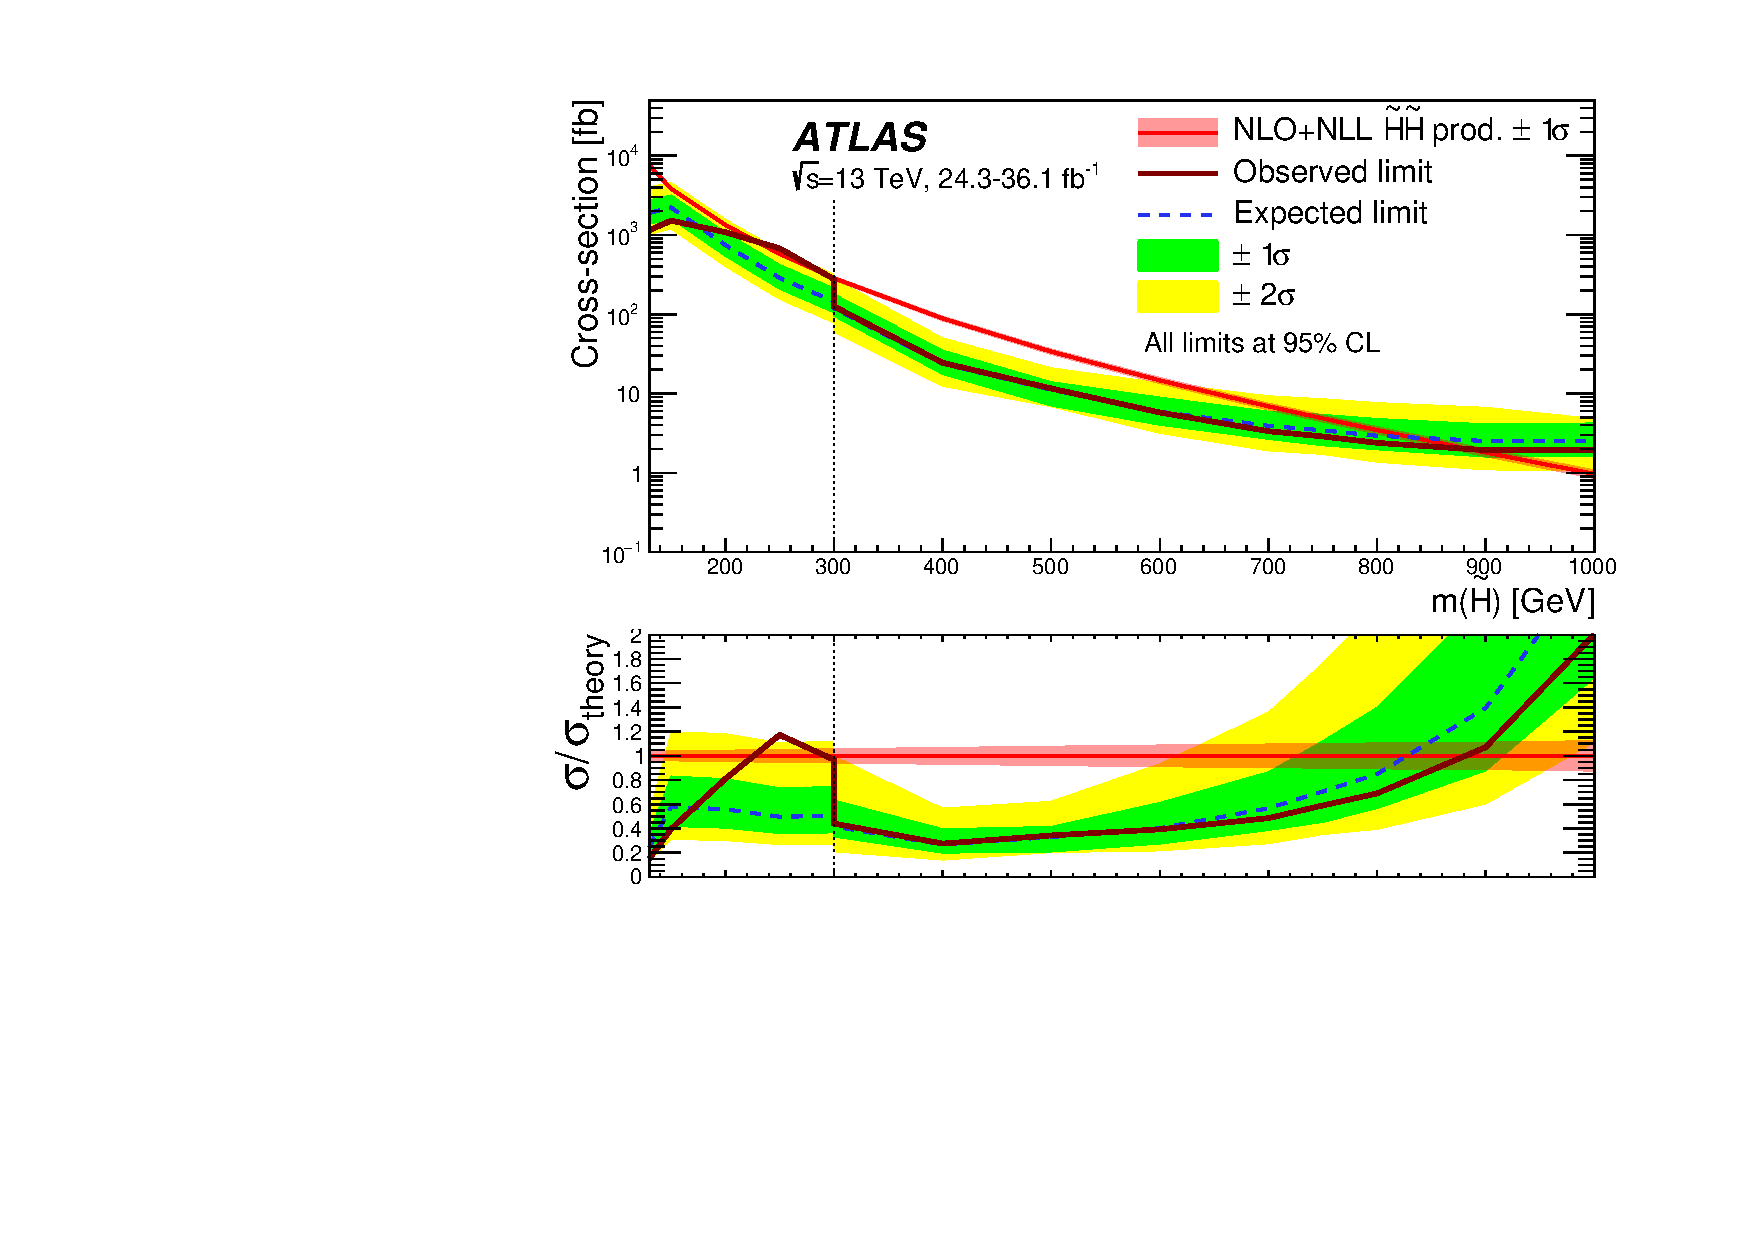
\includegraphics[width=0.75\textwidth]{figures/ewk_prod/interpretation/GGMupperLimit_unblinded_jump}
	\caption{The observed (solid) vs expected (dashed) 95\% upper limits on the \hino\ pair production cross-section as a function of \mhino.  The 1$\sigma$ and 2$\sigma$ uncertainty bands on the expected limit are shown as green and yellow, respectively. The theory cross-section and its uncertainty are shown in the solid and shaded red curve.
   The results of the low-mass analysis are used below $\mhino = 300$ GeV, while those of the high-mass analysis are used above. 
   Figure from Ref. \cite{Aaboud:2018htj}. } 
	\label{fig:ewk:exclusion_comb}
\end{figure}


\begin{figure}[htbp]    
	\centering    
    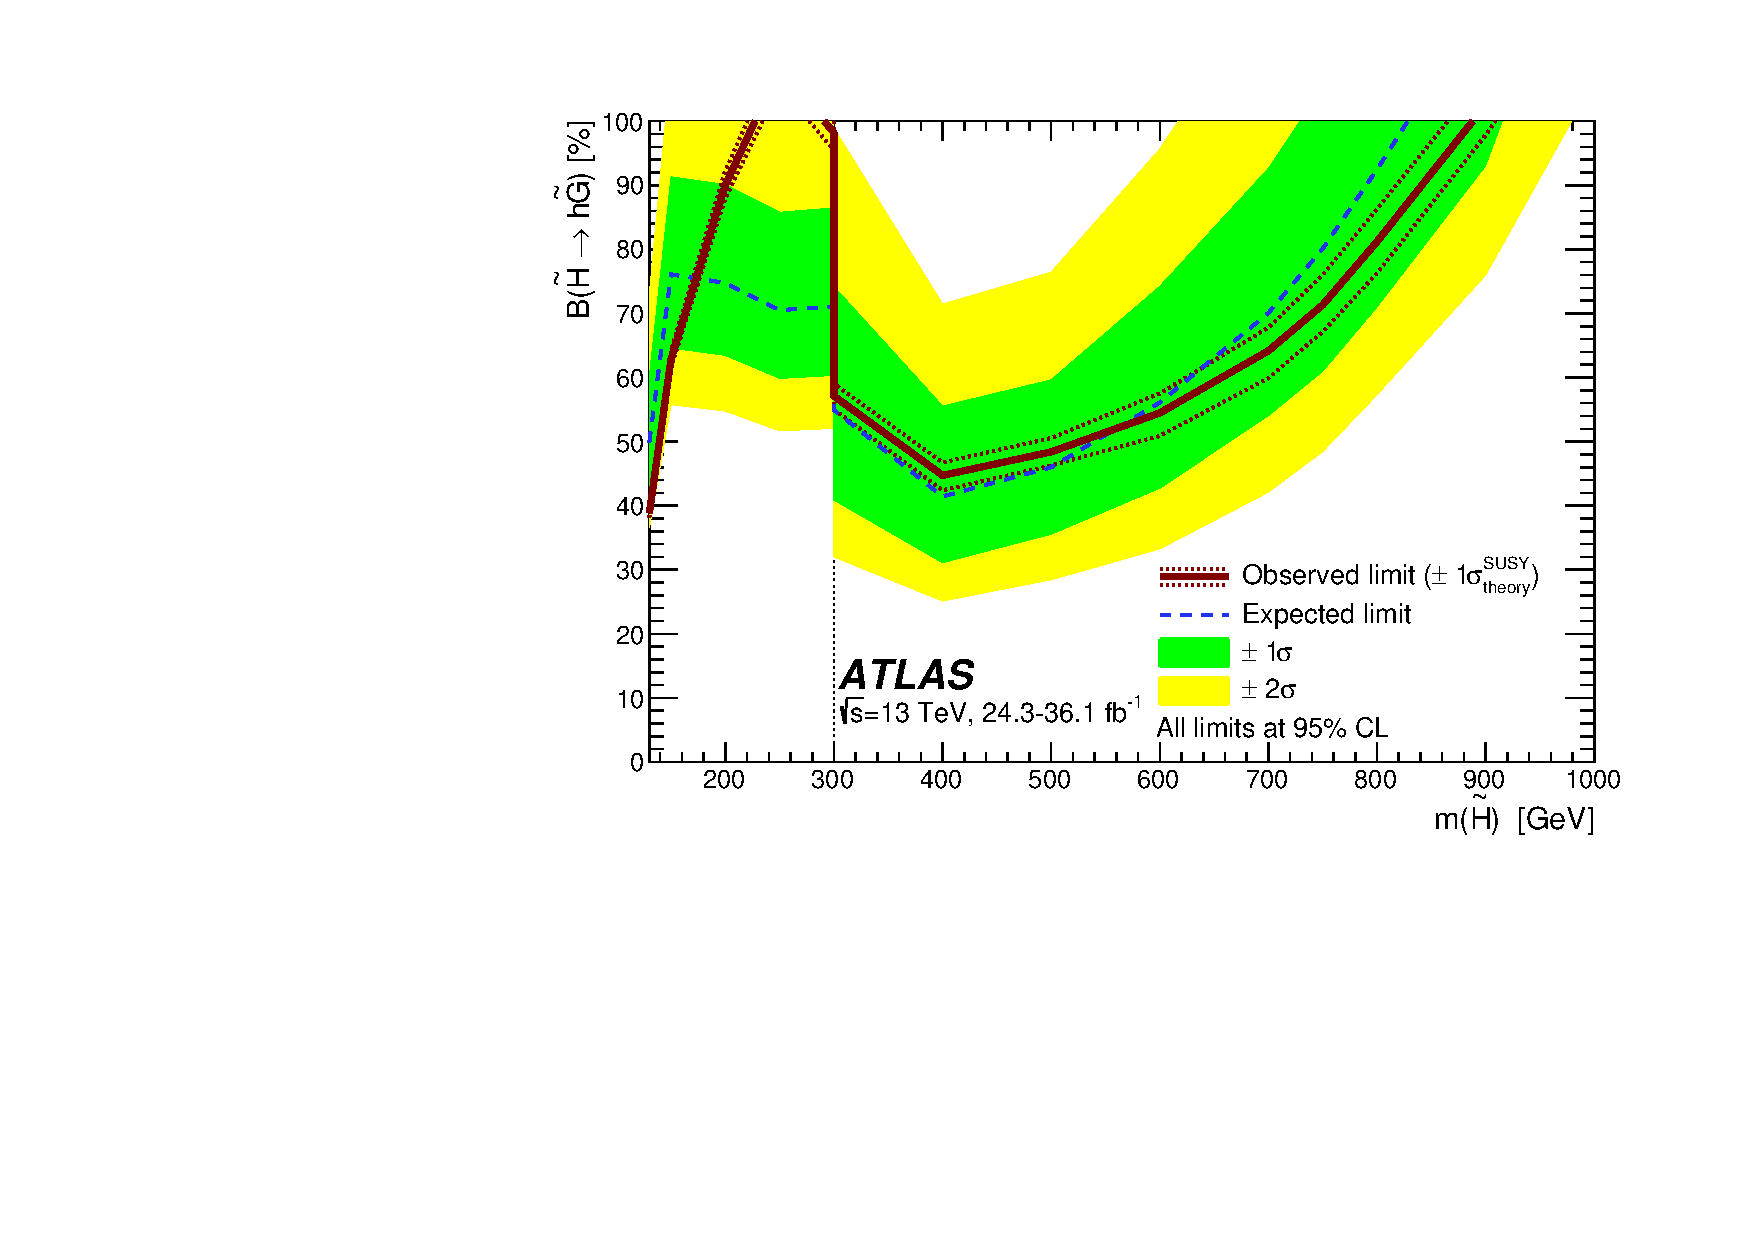
\includegraphics[width=0.75\textwidth]{figures/ewk_prod/interpretation/my_br_plot_unblind_yellow_band}\label{fig:exclusion_br}
	\caption{The observed (solid) vs expected (dashed) 95\% limits in the \mhino\ vs $B(\hino\rightarrow h \tilde{G})$ plane, where $B(\hino\rightarrow h \tilde{G})$ denotes the branching ratio for the decay $\hino \rightarrow h \gravino$. The 1$\sigma$ uncertainty band is overlaid in green and the 2$\sigma$ in yellow.
	The results of the low-mass analysis are used below $\mhino = 300$ GeV, while those of the high-mass analysis are used above.
	 The regions above the lines are excluded by the analyses. Figure from Ref. \cite{Aaboud:2018htj}. } 
	\label{fig:ewk:exclusion_combBR}
\end{figure}



%\section{Results in the Context of the ATLAS SUSY Group}


\clearpage 
\bibliographystyle{atlasBibStyleWithTitle}
\addcontentsline{toc}{section}{Bibliography}
\bibliography{main}
